\documentclass[xcolor=table]{beamer}
\usetheme{uic}
\usepackage{minted}
\usepackage{amsfonts,amsmath,oldgerm,algorithmic,algorithm}
\usepackage[font=small,labelfont=bf]{caption} % Required for specifying captions to tables and figures
\usepackage{tcolorbox}
\tcbuselibrary{listings,skins}
\usepackage{alltt,xcolor}
\usepackage{hyperref}
\usepackage{comment}
\usepackage{amsthm}
\usepackage[spanish]{babel}


\lstdefinestyle{mystyle}{
language=C
}

\newtcblisting{mylisting}[2][]{
    arc=0pt, outer arc=0pt,
    listing only, 
    listing style=mystyle,
    title=#2,
    #1
}


\newcommand{\hrefcol}[2]{\textcolor{uihteal}{\href{#1}{#2}}}
\newcommand{\testcolor}[1]{\colorbox{#1}{\textcolor{#1}{test}}~\texttt{#1}}

% Please see Section 18.1 of Beamer User Guide for all the options \usefonttheme provides
\usefonttheme[onlymath]{serif}
% \usefonttheme{serif} % use this if you would like Serif font throughout (and not just for math)

\title{Fundamentos de Inteligencia Artificial}
\titlebackground{images/etsiinformatica3.jpeg}
% an asterisk will split the background:
% \titlebackground*{images/uic_seo.jpg}
\subtitle{Búsqueda heurística avanzada y MultiAgentes}

\author{\href{mailto:jmmontes@uma.es}{José A. Montenegro}}
\date{\today}

%https://aima.cs.berkeley.edu/algorithms.pdf


\begin{document}

\newtheorem{mydef}{Definición}[section] % Añade [section] para que se reinicie en cada sección
\maketitle

% default is no footline, but page numbers are incredibly useful for the audience to ask questions later
\footlinecolor{uicblue}

%%%%%%%%%%%%%%%%%%%%%%%%%%%%%%%%%%%%%%%%%%%%%%%%%%%
%%%%%%%%%%%%%%%%%%%%%%%%%%%%%%%%%%%%%%%%%%%%%%%%%%%
%%%%%%%%%%%%%%%%%%%%%%%%%%%%%%%%%%%%%%%%%%%%%%%%%%%
%%%%%%%%%%%%%%%%%%%%%%%%%%%%%%%%%%%%%%%%%%%%%%%%%%%
%%%%%%%%%%%%%%%%%%%%%%%%%%%%%%%%%%%%%%%%%%%%%%%%%%%
%%%%%%%%%%%%%%%%%%%%%%%%%%%%%%%%%%%%%%%%%%%%%%%%%%%


%%%%%%%%%%%%%%%%%%%%%%%%%%%%%%%%%%%%%%%%%%%%%%%%%%%
%%%%%%%%%%%%%%%%%%%%%%%%%%%%%%%%%%%%%%%%%%%%%%%%%%%
%%%%%%%%%%%%%%%%%%%%%%%%%%%%%%%%%%%%%%%%%%%%%%%%%%%
%%%%%%%%%%%%%%%%%%%%%%%%%%%%%%%%%%%%%%%%%%%%%%%%%%%
%%%%%%%%%%%%%%%%%%%%%%%%%%%%%%%%%%%%%%%%%%%%%%%%%%%
%%%%%%%%%%%%%%%%%%%%%%%%%%%%%%%%%%%%%%%%%%%%%%%%%%%


\begin{frame}{Contenido}
\tableofcontents
\end{frame}

%%%%%%%%%%%%%%%%%%%%%%%%%%%%%%%%
%%%%%%%%%%%%%%%%%%%%%%%%%%%%%%%%
%SECCION %%%%%%%%%%%%%%%%%%%%%%%%%%%%%%%
%%%%%%%%%%%%%%%%%%%%%%%%%%%%%%%%
%%%%%%%%%%%%%%%%%%%%%% 

\begin{chapter}[images/etsiinformatica4.png]{uicblue}{$IDA^*$}
\end{chapter}

\section{Búsqueda heurística avanzada}
\subsection{IDA*}
%%%%%%%%%%%%%%%%%%%%%%%%%%%%%%%%
%%%%%%%%%%%%%%%%%%%%%%%%%%%%%%%%
%%%%%%%%%%%%%%%%%%%%%%%%%%%%%%%%

%%%%%%%%%%%%%%%%%%%%%%%%%%%%%%%%
%%%%%%%%%%%%%%%%%%%%%%%%%%%%%%%%

%%%%%%%%%%%%%%%%%%%%%%%%%%%%%%%%
\begin{frame} \frametitle{$IDA^*$} \small

\begin{itemize}
    \item Iterative-deepening $A^*$ ($IDA^*$) dónde el límite de la búsqueda es definida utilizando la función de coste f(n) en vez de la profundidad.
    \item $IDA^*$ nos da las ventajas de $A^*$ sin el requisito de mantener todos los estados alcanzados en memoria, 
    \item Por contramedida, vamos a visitar algunos estados varias veces. 
    \item Es un algoritmo muy importante comúnmente utilizado para problemas que no caben en memoria.

\end{itemize}
\end{frame} 


%%%%%%%%%%%%%%%%%%%%%%%%%%%%%%%%
\begin{frame} \frametitle{$IDA^*$} \small


\begin{figure}
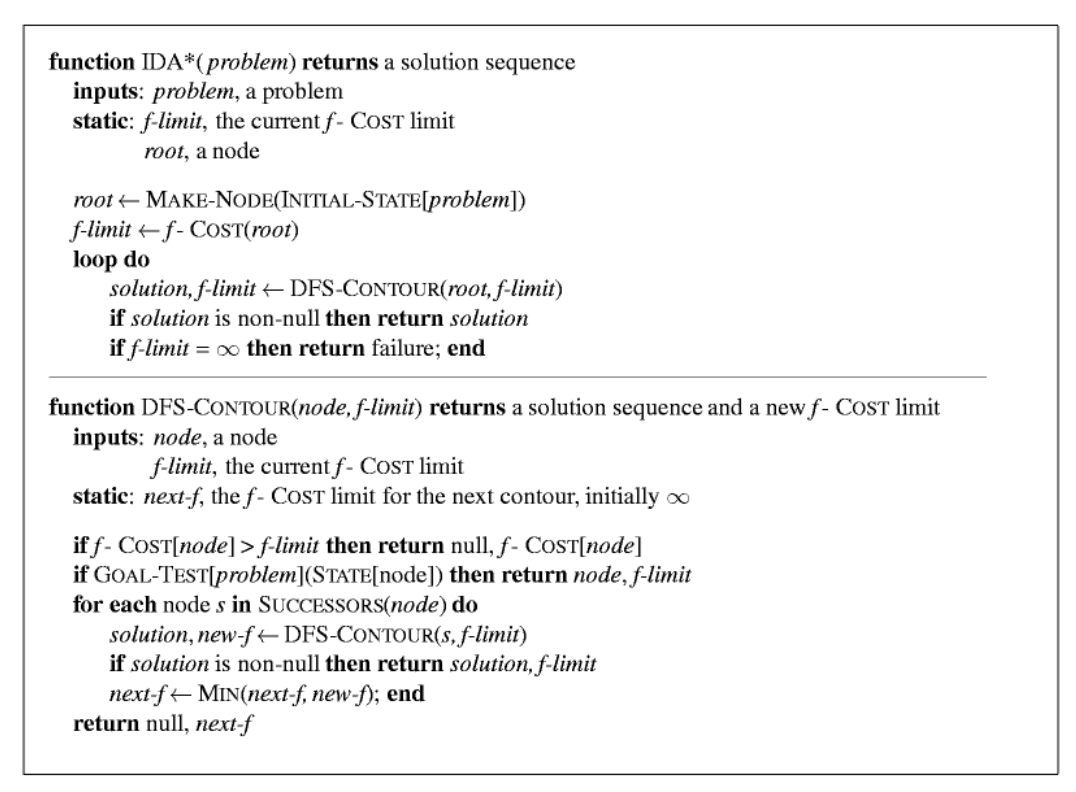
\includegraphics[scale=0.4]{./img/IDA}
\end{figure}


\end{frame} 
%%%%%%%%%%%%%%%%%%%%%%%%%%%%%%%%

\begin{frame} [fragile ]\frametitle{IDA* en Python } \footnotesize
\begin{minted}[fontsize=\footnotesize]{python}

def ida_star(problem):
    bound = problem.f(Node(problem.initial_state))
    path = [Node(problem.initial_state)]
    while True:
        result, new_bound = depth_limited_search(problem, bound, path)
        if result == 'FOUND':
            return path
        if result == float('inf'):
            return 'No se encontró camino'
        bound = new_bound
        print("\n\n new bound", bound)

\end{minted}

\end{frame} 

%%%%%%%%%%%%%%%%%%%%%%%%%%%%%%%%
\begin{frame} [fragile ]\frametitle{IDA* en Python } \footnotesize
\begin{minted}[fontsize=\tiny]{python}

def depth_limited_search(problem, bound, path,):

    node = path[-1]
    f = problem.f(node)    
    print("NODE", node, "f",f)  
    if problem.f(node) > bound:
        print("\t Poda NODE", node, "f",f)
        return f, 0
    if problem.is_goal(node.state):
        return 'FOUND', 0

    min_val = float('inf')
    for child_state, cost in problem.expand(node.state):
        if child_state not in [n.state for n in path]:
            child_node = Node(child_state, node, node.cost + cost)  
            path.append(child_node)
            result, _ = depth_limited_search(problem, bound, path)
            if result == 'FOUND':
                return 'FOUND', 0
            if result < min_val:
                min_val = result
            path.pop()
    return min_val, min_val

\end{minted}

\end{frame} 

%%%%%%%%%%%%%%%%%%%%%%%%%%%%%%%%
%%%%%%%%%%%%%%%%%%%%%%%%%%%%%%%%
%%%%%%%%%%%%%%%%%%%%%%%%%%%%%%%%
\begin{chapter}[images/etsiinformatica4.png]{uicblue}{$IDA^*$\\
Ejemplo Grafo}
\end{chapter}

%%%%%%%%%%%%%%%%%%%%%%%%%%%%%%%%
\begin{frame} \frametitle{Ejemplo Grafo} \small
\begin{figure}
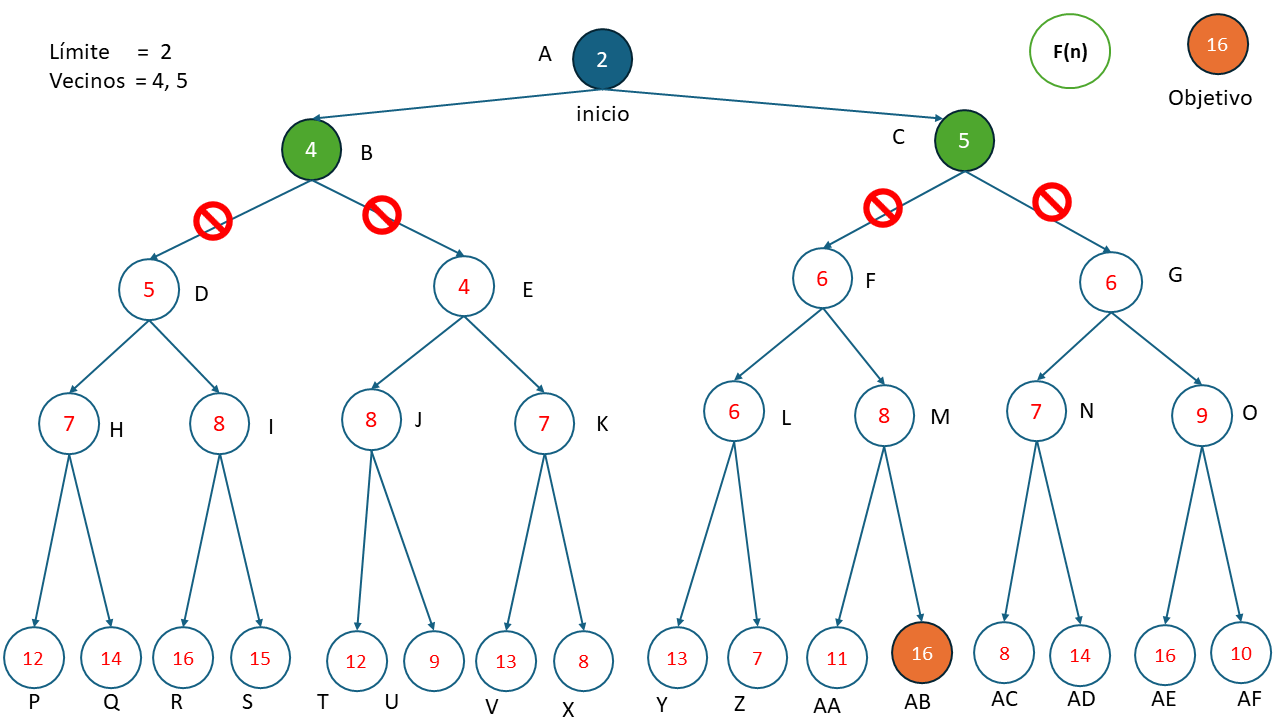
\includegraphics[scale=0.3]{./img/GrafoIDA1}
\end{figure}
\end{frame} 

\begin{frame} \frametitle{Ejemplo Grafo} \small
\begin{figure}
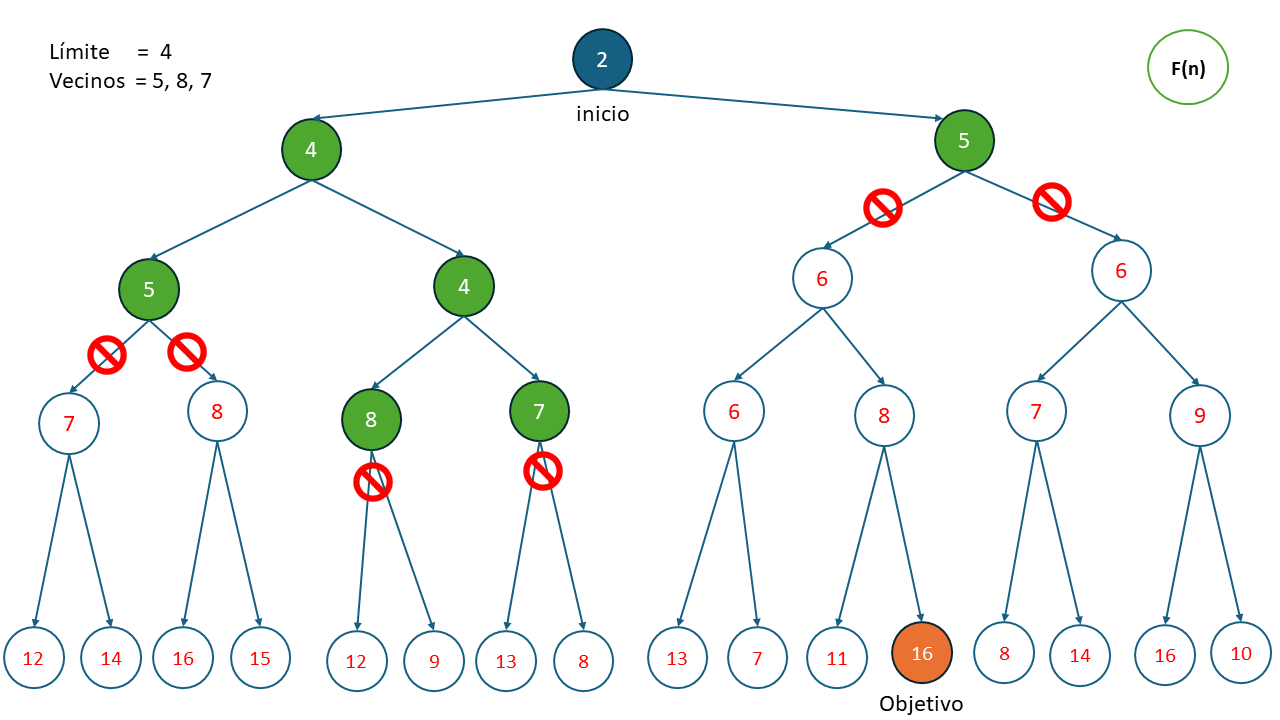
\includegraphics[scale=0.3]{./img/GrafoIDA2}
\end{figure}
\end{frame} 

\begin{frame} \frametitle{Ejemplo Grafo} \small
\begin{figure}
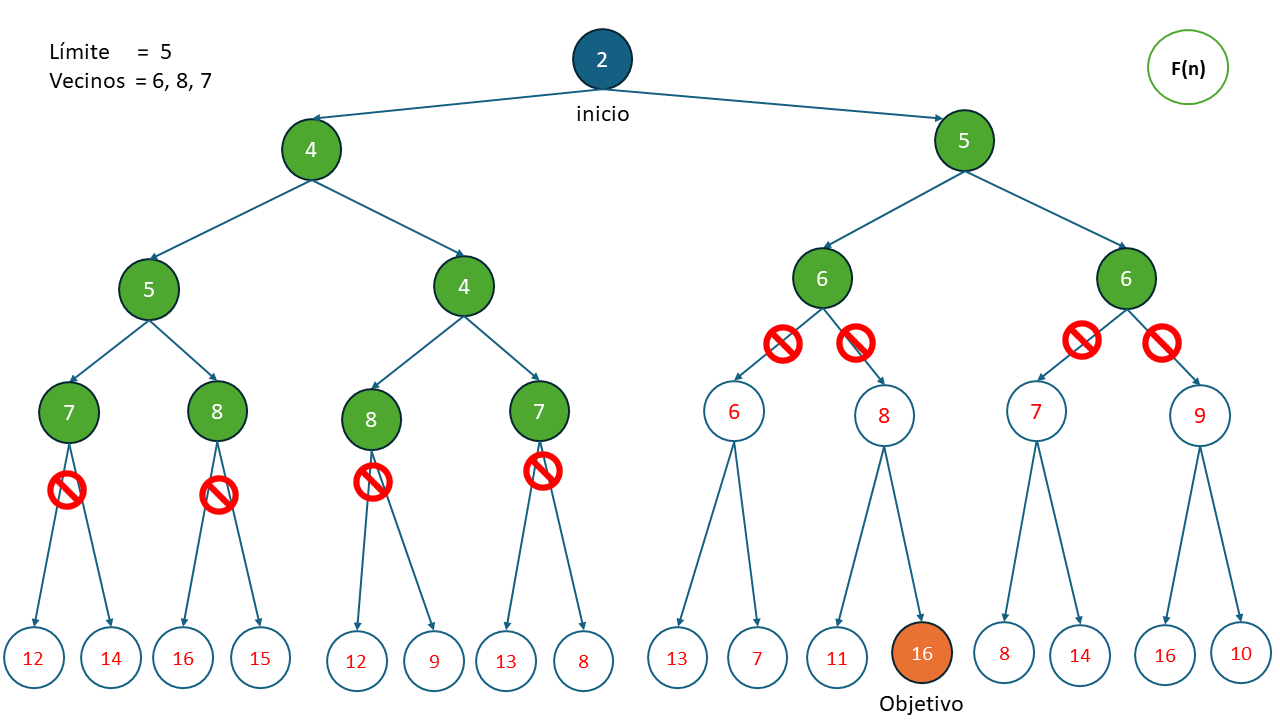
\includegraphics[scale=0.3]{./img/GrafoIDA3}
\end{figure}
\end{frame} 

\begin{frame} \frametitle{Ejemplo Grafo} \small
\begin{figure}
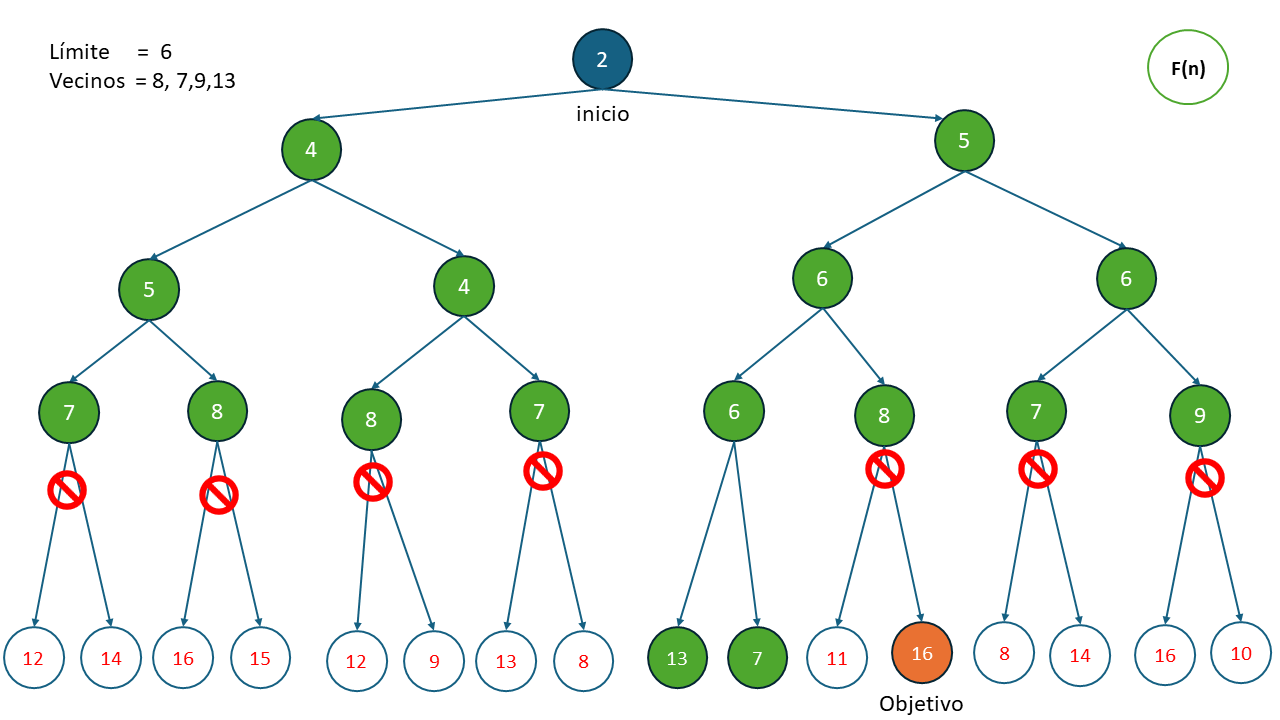
\includegraphics[scale=0.3]{./img/GrafoIDA4}
\end{figure}
\end{frame} 


\begin{frame} \frametitle{Ejemplo Grafo} \small
\begin{figure}
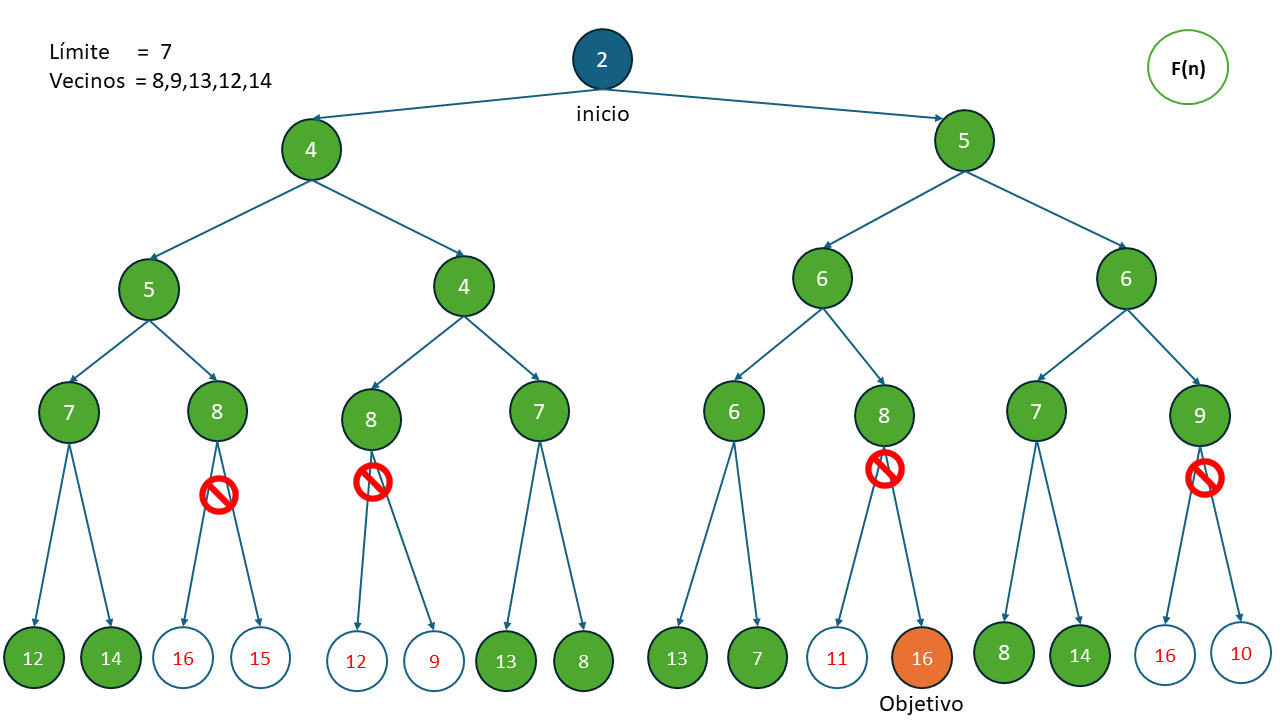
\includegraphics[scale=0.3]{./img/GrafoIDA5}
\end{figure}
\end{frame} 

\begin{frame} \frametitle{Ejemplo Grafo} \small
\begin{figure}
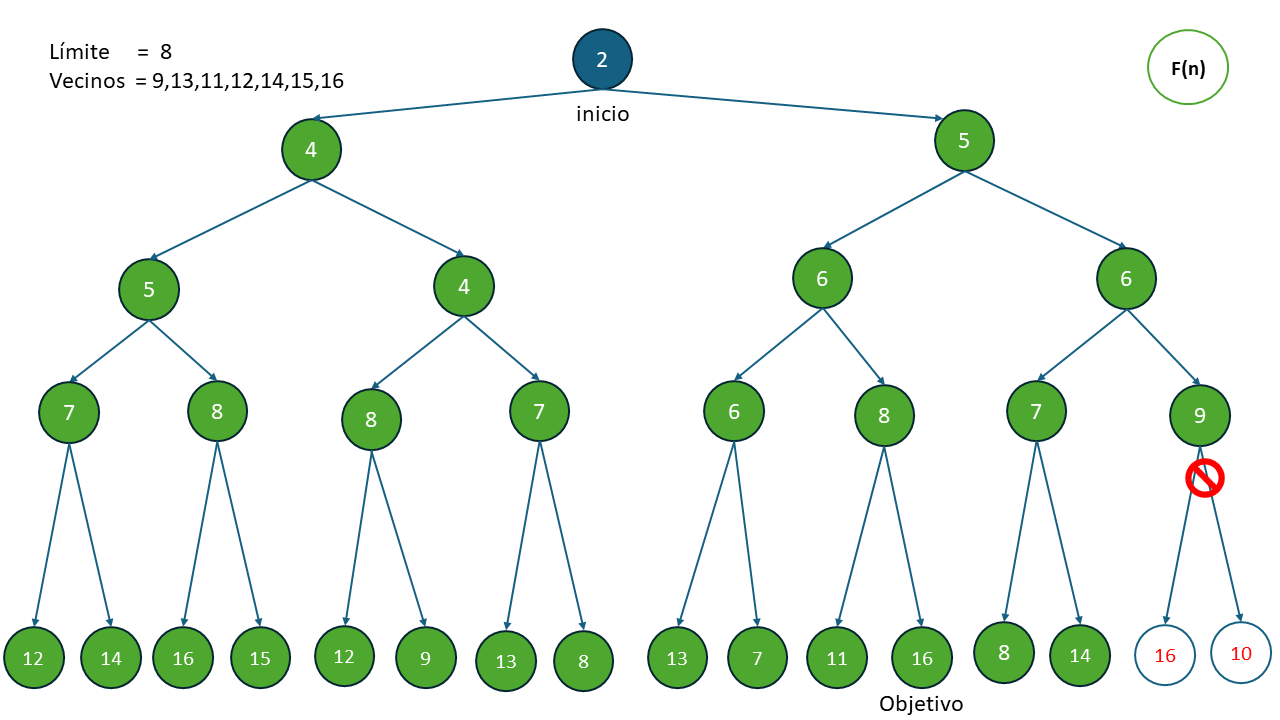
\includegraphics[scale=0.3]{./img/GrafoIDA6}
\end{figure}
\end{frame} 

\begin{frame} \frametitle{Ejemplo Grafo} \small
\begin{figure}
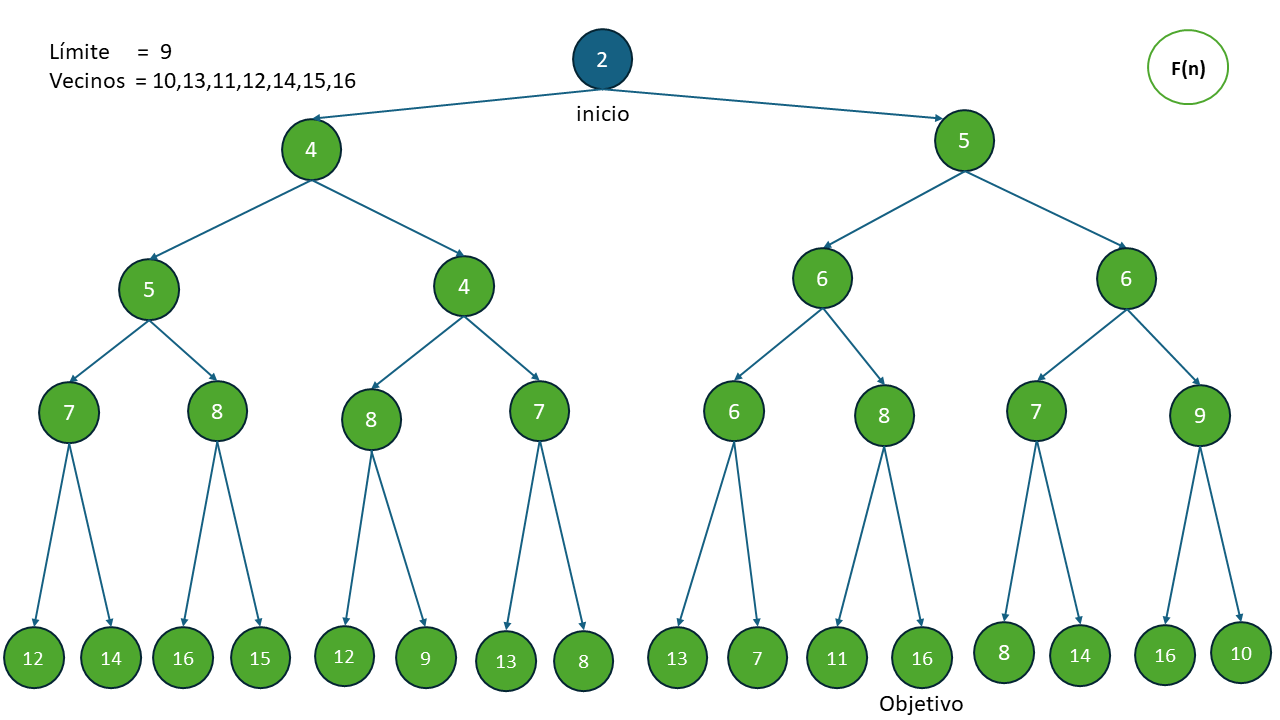
\includegraphics[scale=0.3]{./img/GrafoIDA7}
\end{figure}
\end{frame} 

\begin{frame} \frametitle{Ejemplo Grafo} \small
\begin{figure}
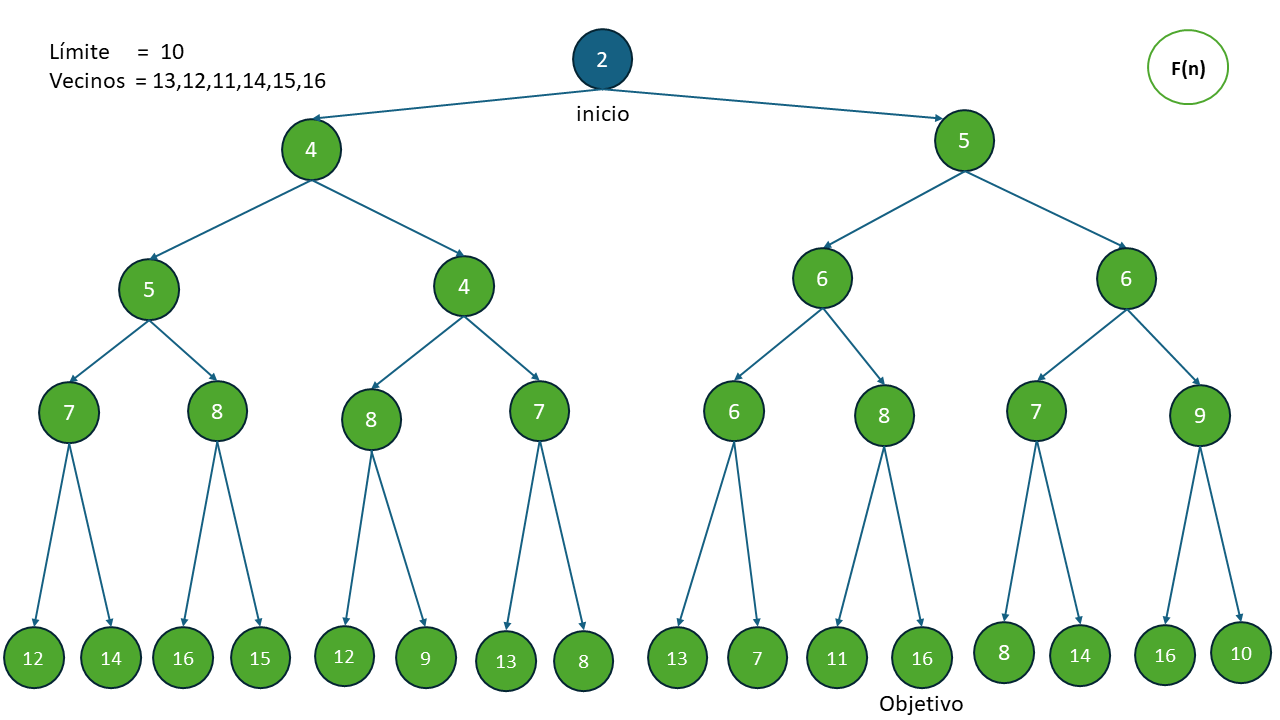
\includegraphics[scale=0.3]{./img/GrafoIDA8}
\end{figure}
\end{frame} 

\begin{frame} \frametitle{Ejemplo Grafo} \small
\begin{figure}
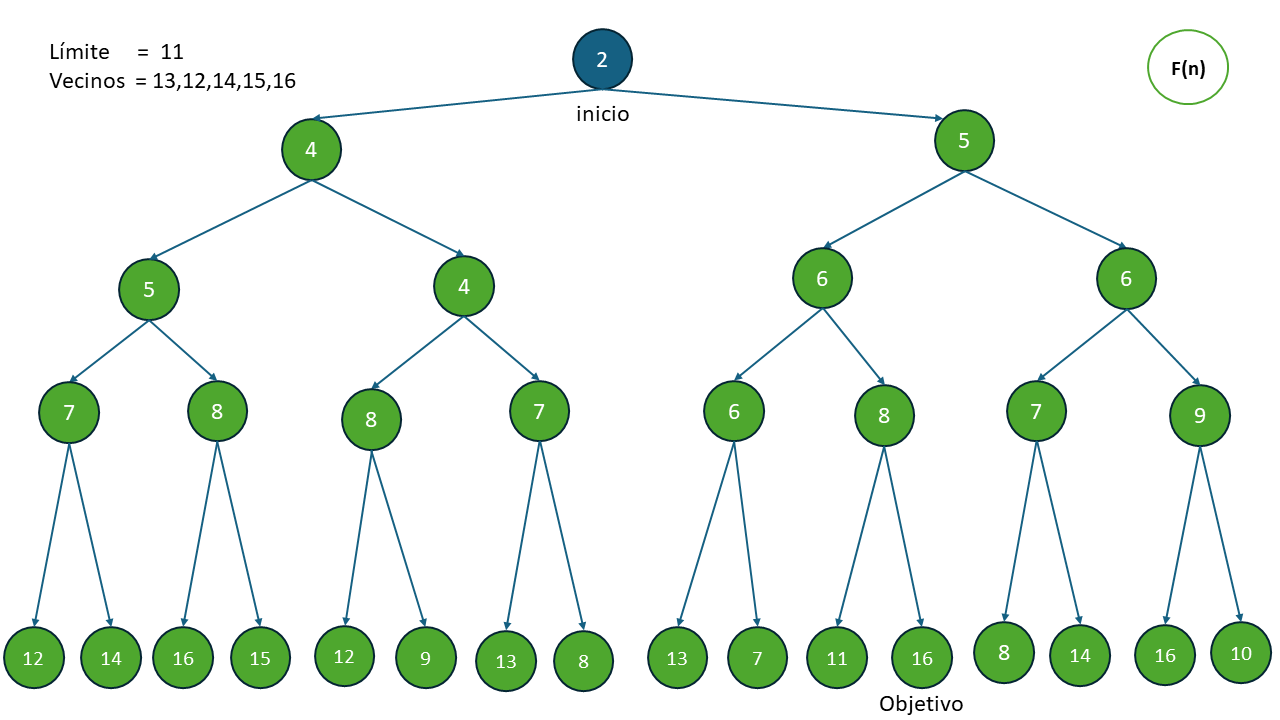
\includegraphics[scale=0.3]{./img/GrafoIDA9}
\end{figure}
\end{frame} 

\begin{frame} \frametitle{Ejemplo Grafo} \small
\begin{figure}
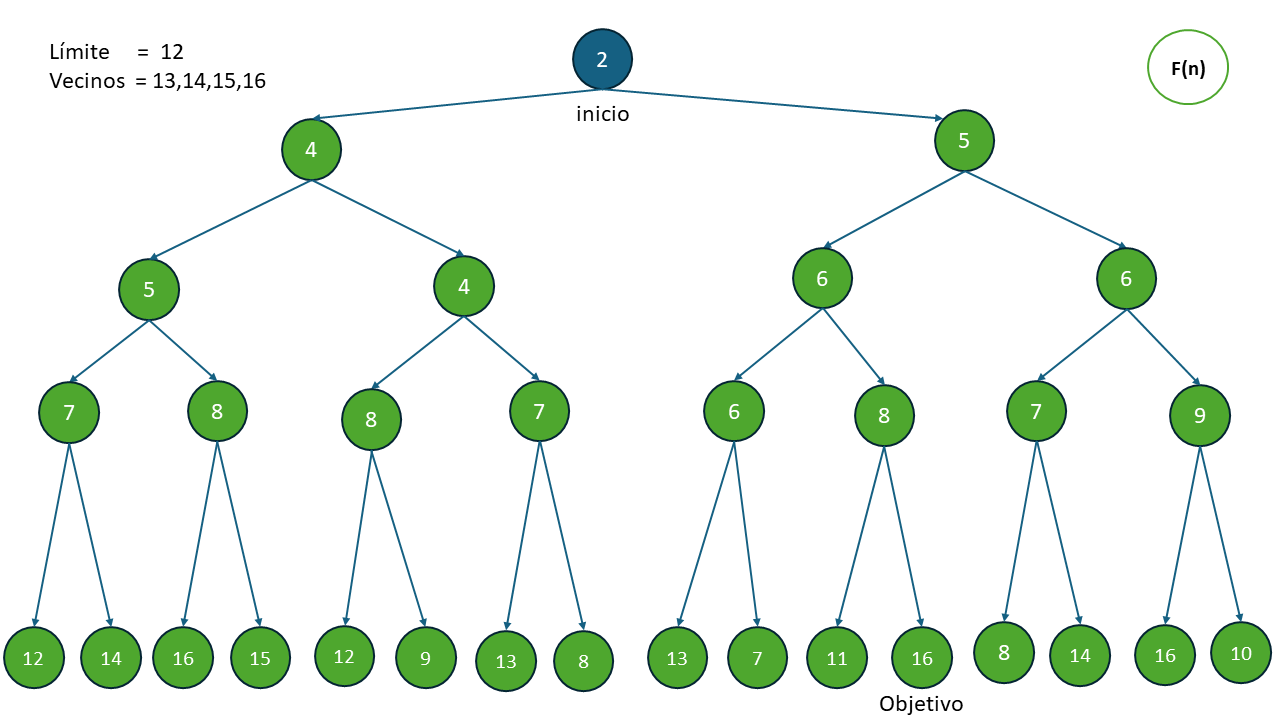
\includegraphics[scale=0.3]{./img/GrafoIDA10}
\end{figure}
\end{frame} 

\begin{frame} \frametitle{Ejemplo Grafo} \small
\begin{figure}
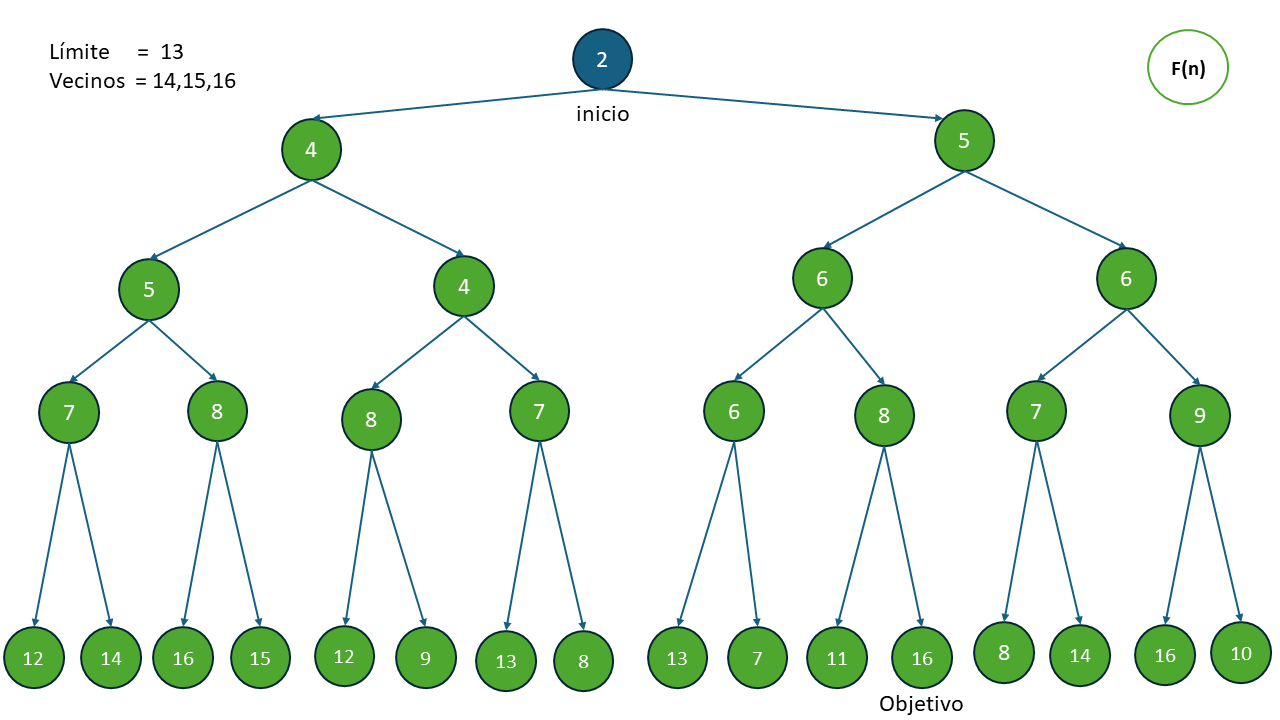
\includegraphics[scale=0.3]{./img/GrafoIDA11}
\end{figure}
\end{frame} 

\begin{frame} \frametitle{Ejemplo Grafo} \small
\begin{figure}
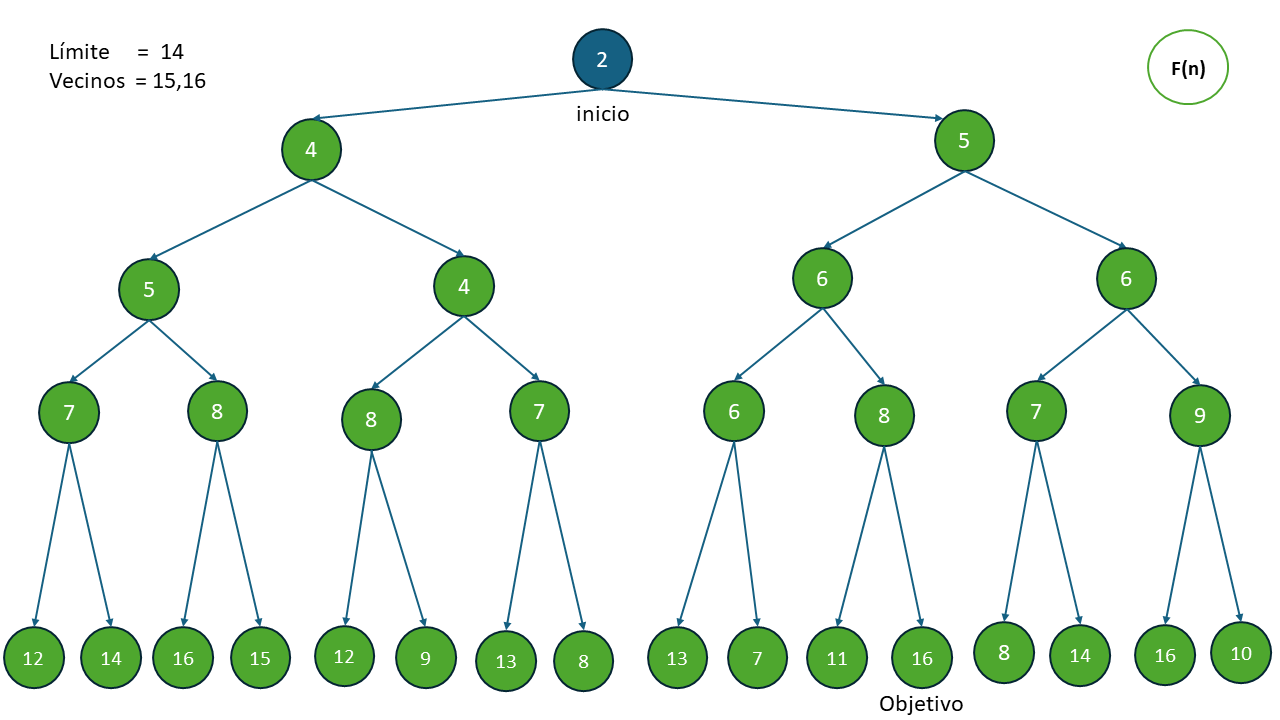
\includegraphics[scale=0.3]{./img/GrafoIDA12}
\end{figure}
\end{frame} 

\begin{frame} \frametitle{Ejemplo Grafo} \small
\begin{figure}
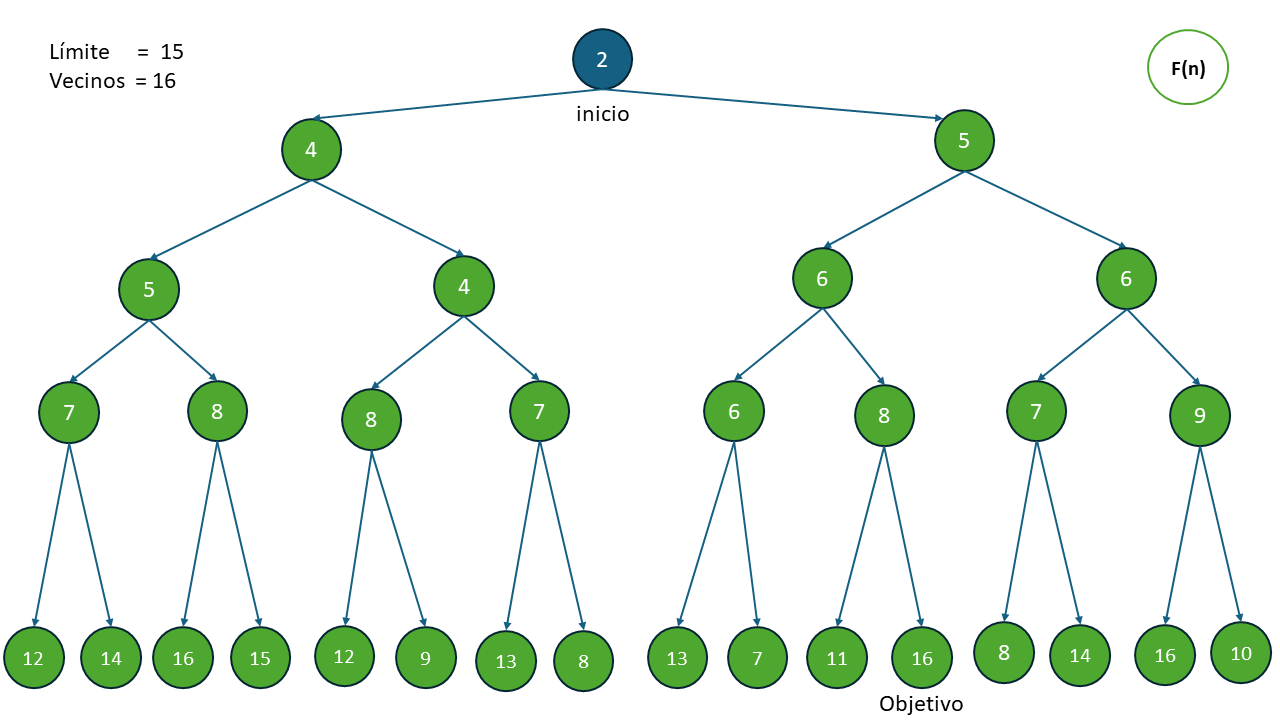
\includegraphics[scale=0.3]{./img/GrafoIDA13}
\end{figure}
\end{frame} 

\begin{frame} \frametitle{Ejemplo Grafo} \small
\begin{figure}
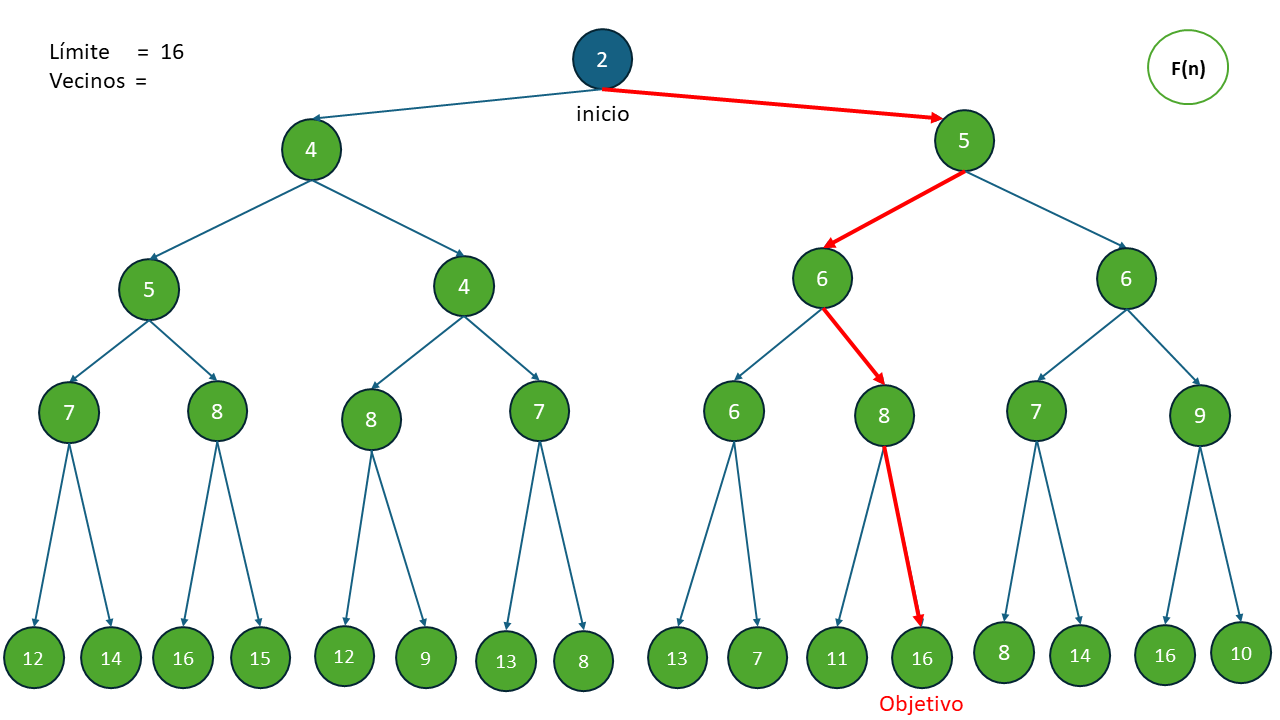
\includegraphics[scale=0.3]{./img/GrafoIDA14}
\end{figure}
\end{frame} 

%%%%%%%%%%%%%%%%%%%%%%%%%%%%%%%%
%%%%%%%%%%%%%%%%%%%%%%%%%%%%%%%%
%%%%%%%%%%%%%%%%%%%%%%%%%%%%%%%%
\begin{chapter}[images/etsiinformatica4.png]{uicblue}{$IDA^*$\\
Ejemplo Rumania}
\end{chapter}

%%%%%%%%%%%%%%%%%%%%%%%%%%%%%%%%

\begin{frame} \frametitle{Ejemplo Rumania} \small
\begin{figure}
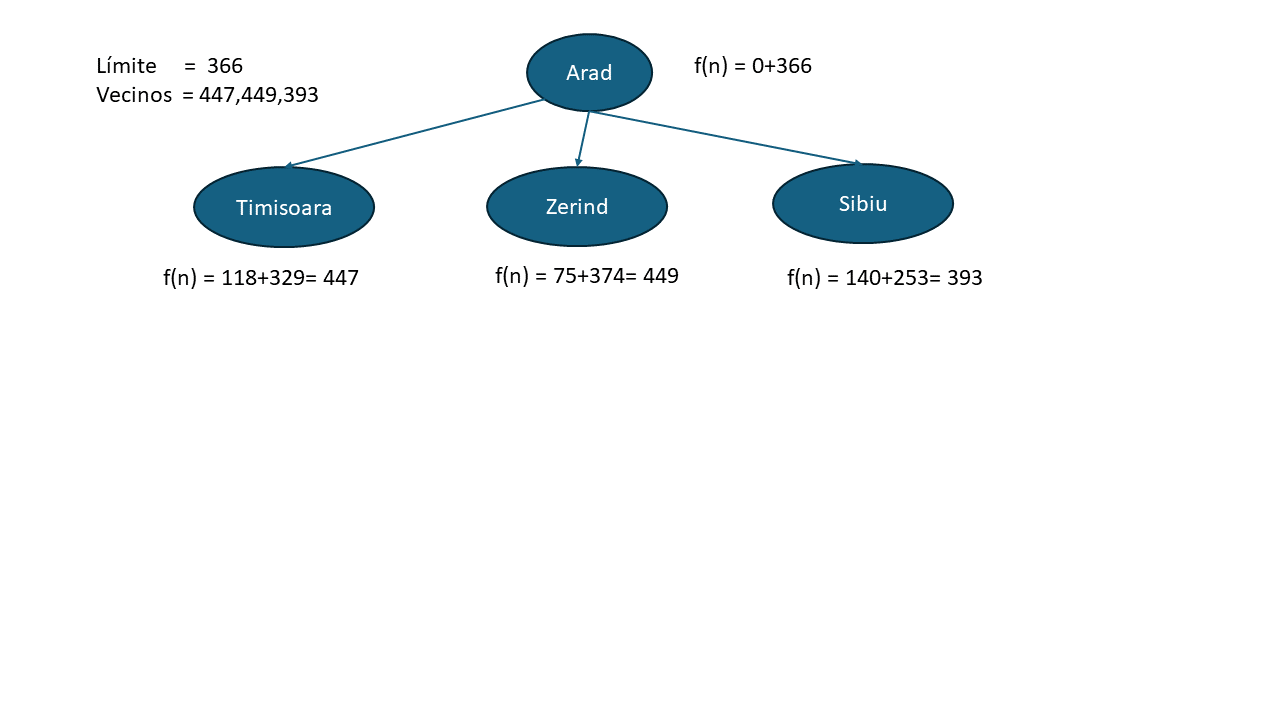
\includegraphics[scale=0.3]{./img/RumaniaIDA1}
\end{figure}
\end{frame} 

\begin{frame} \frametitle{Ejemplo Rumania} \small
\begin{figure}
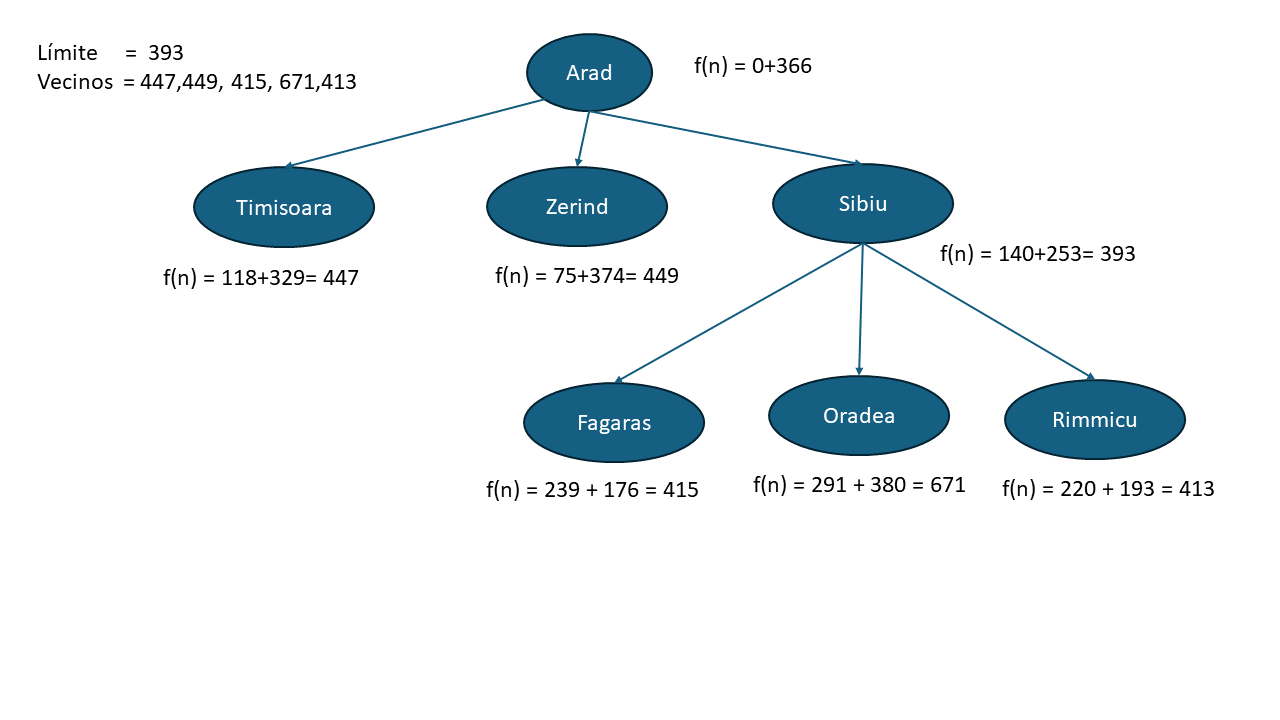
\includegraphics[scale=0.3]{./img/RumaniaIDA2}
\end{figure}
\end{frame} 

\begin{frame} \frametitle{Ejemplo Rumania} \small
\begin{figure}
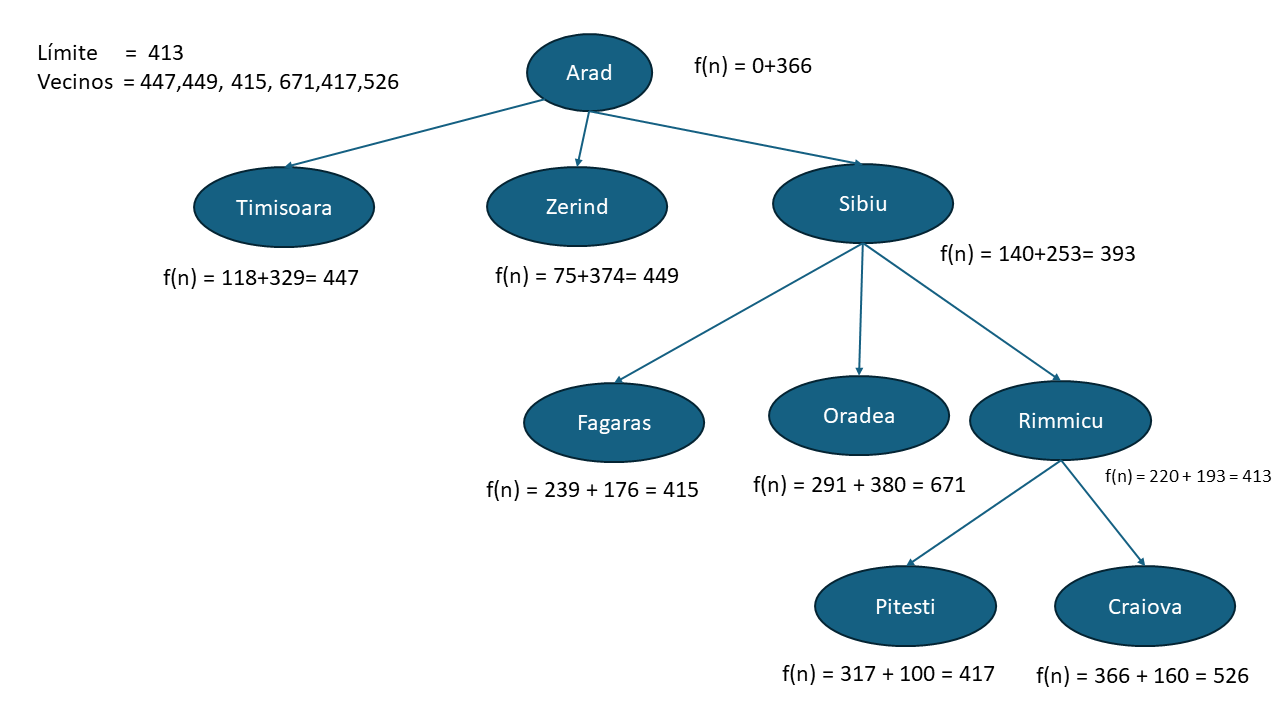
\includegraphics[scale=0.3]{./img/RumaniaIDA3}
\end{figure}
\end{frame} 

\begin{frame} \frametitle{Ejemplo Rumania} \small
\begin{figure}
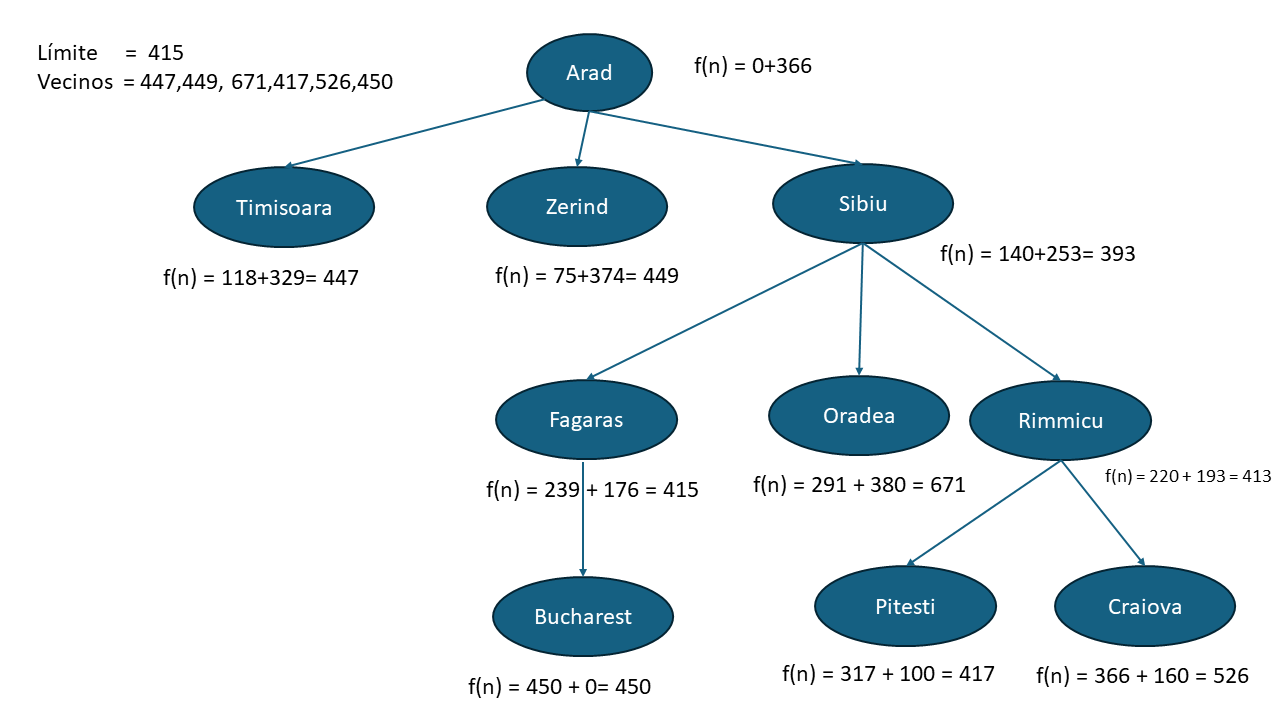
\includegraphics[scale=0.3]{./img/RumaniaIDA4}
\end{figure}
\end{frame} 

\begin{frame} \frametitle{Ejemplo Rumania} \small
\begin{figure}
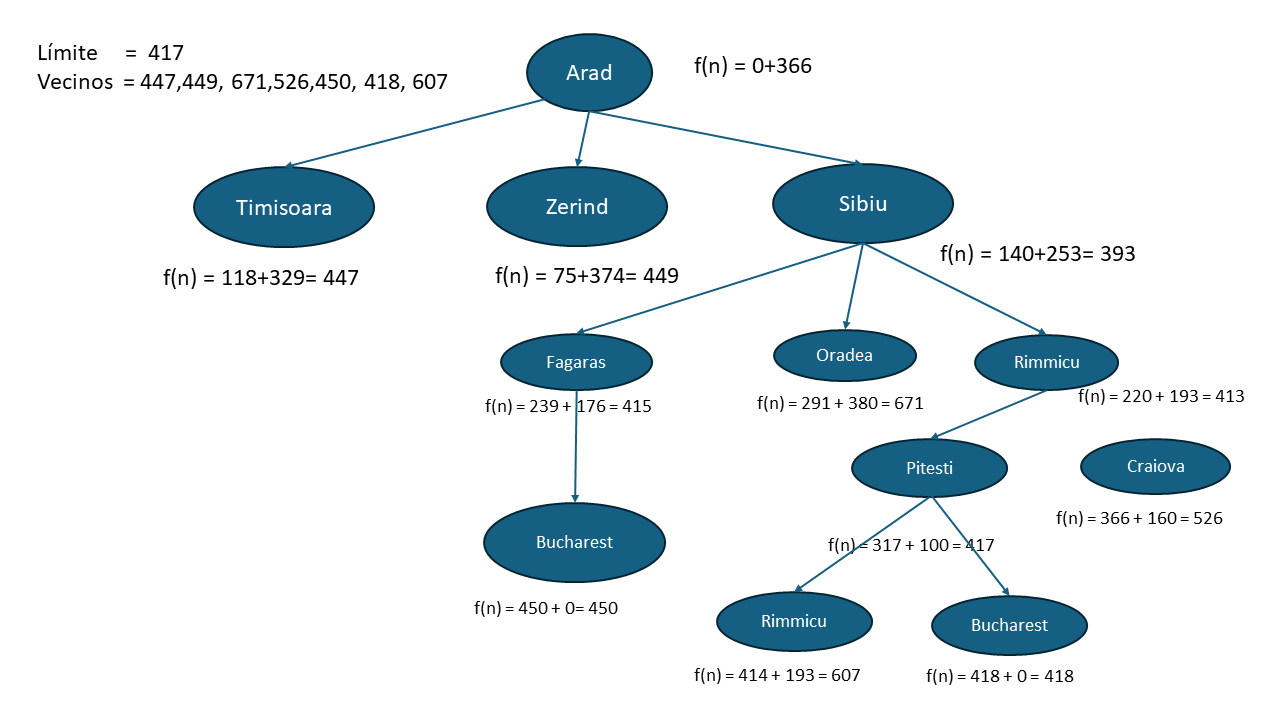
\includegraphics[scale=0.3]{./img/RumaniaIDA5}
\end{figure}
\end{frame} 

\begin{frame} \frametitle{Ejemplo Rumania} \small
\begin{figure}
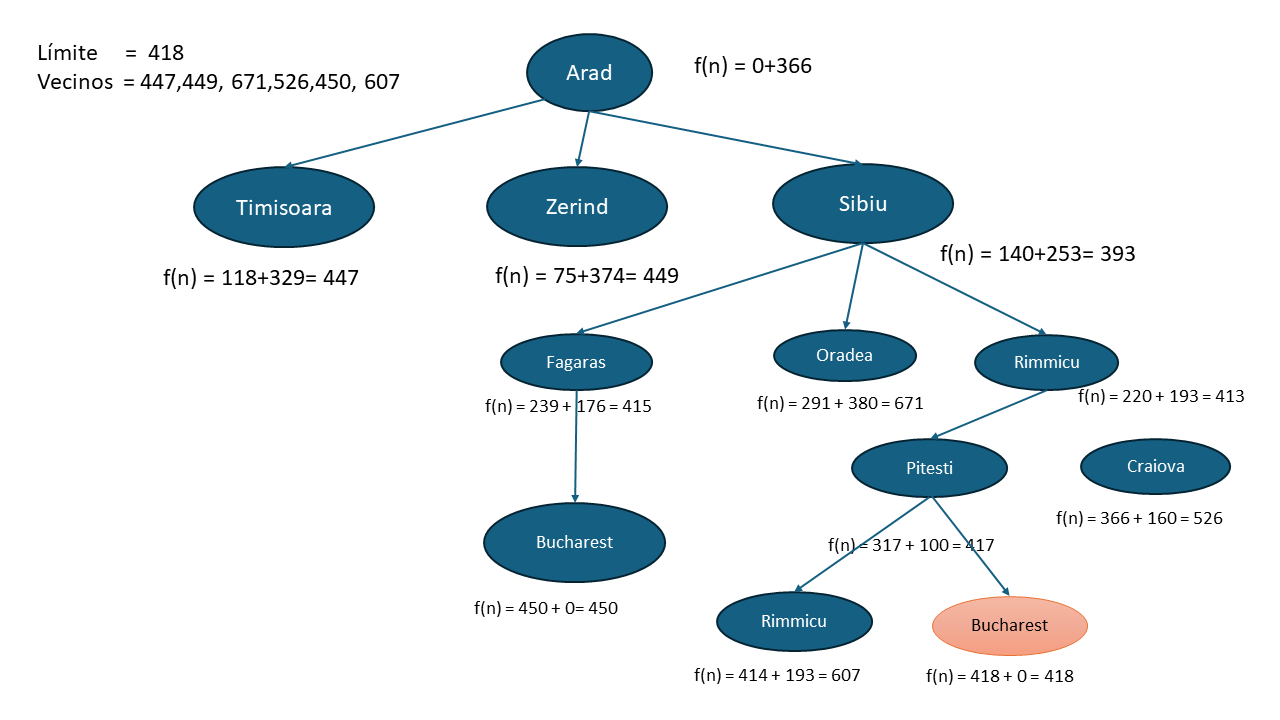
\includegraphics[scale=0.3]{./img/RumaniaIDA6}
\end{figure}
\end{frame} 

\subsection{Pathfinding}




\begin{chapter}[images/etsiinformatica4.png]{uicblue}{ Path Finding}
\end{chapter}

%%%%%%%%%%%%%%%%%%%%%%%%%%%%%%%%
\begin{frame} \frametitle{ Path Finding} \small

\begin{itemize}
\item Camino desde un nodo origen a un nodo destino, evitando obstáculos,  sobre un mapa que está dividido en cuadrículas. 
\item Los movimientos permitidos en cada paso desde estado actual, dependen del problema:
\end{itemize}

\begin{figure}
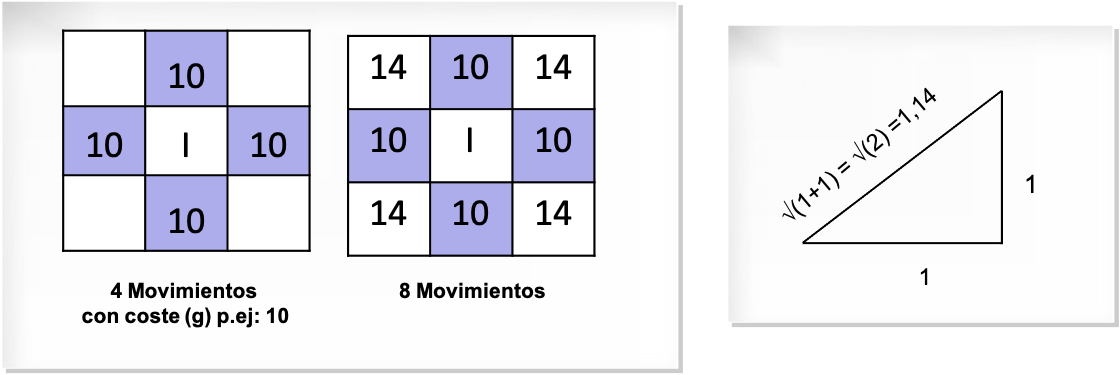
\includegraphics[scale=0.45]{./img/PathFinding}
\end{figure}

\end{frame} 

%%%%%%%%%%%%%%%%%%%%%%%%%%%%%%%%

\begin{frame} \frametitle{Ejemplo Path Finding 4 Movimientos} \small

\begin{figure}
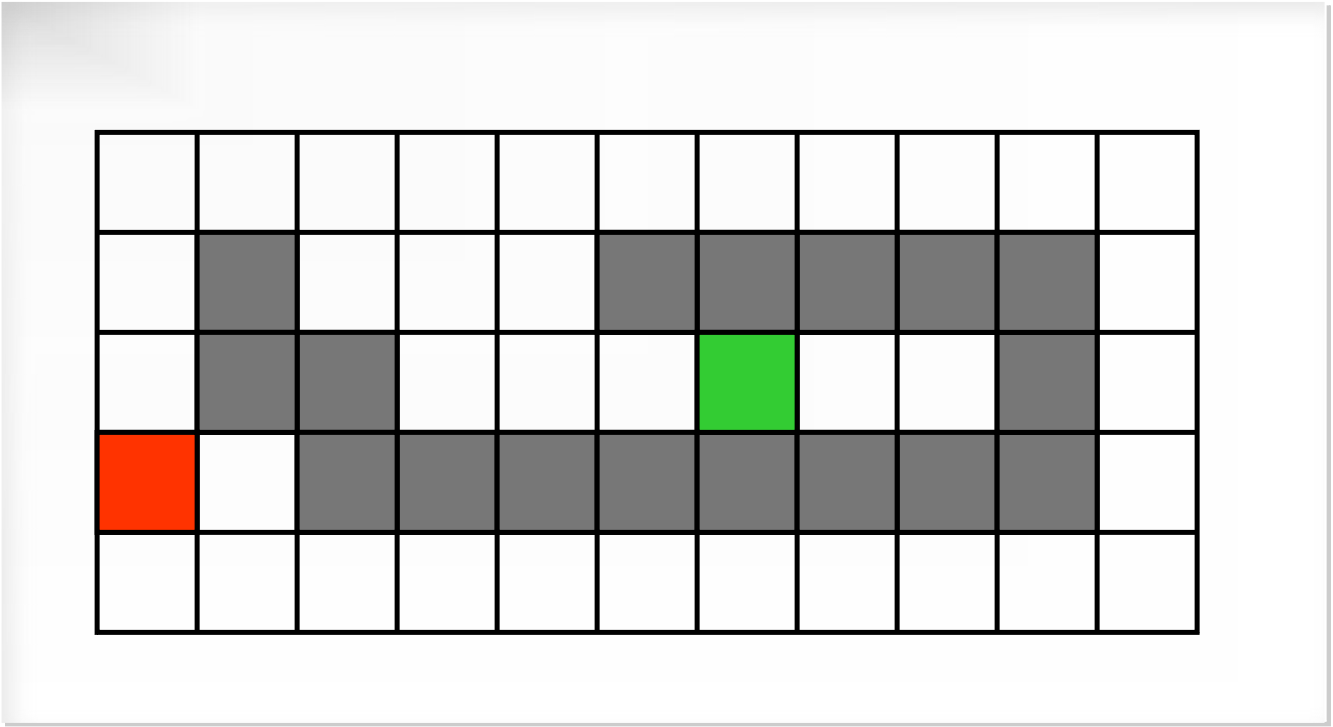
\includegraphics[scale=0.4]{./img/EjemploA1}
\end{figure}

\end{frame} 
%%%%%%%%%%%%%%%%%%%%%%%%%%%%%%%%

\begin{frame} \frametitle{Ejemplo Path Finding 4 Movimientos} \small

\begin{center}
f(N) = h(N), con h(N) = Distancia Manhattan al objetivo
\end{center}

\begin{figure}
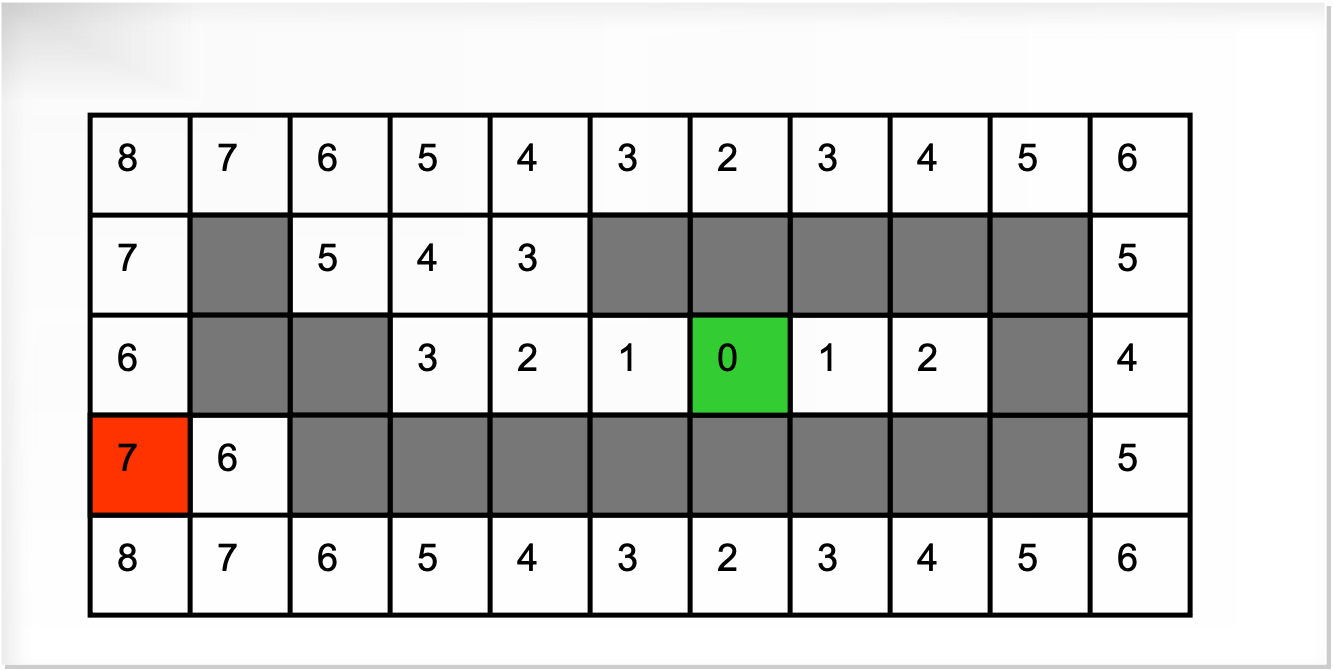
\includegraphics[scale=0.4]{./img/EjemploA2}
\end{figure}

\end{frame} 
%%%%%%%%%%%%%%%%%%%%%%%%%%%%%%%%

\begin{frame} \frametitle{Ejemplo Path Finding 4 Movimientos} \small

\begin{center}
f(N) = h(N), con h(N) = Distancia Manhattan al objetivo
\end{center}


\begin{figure}
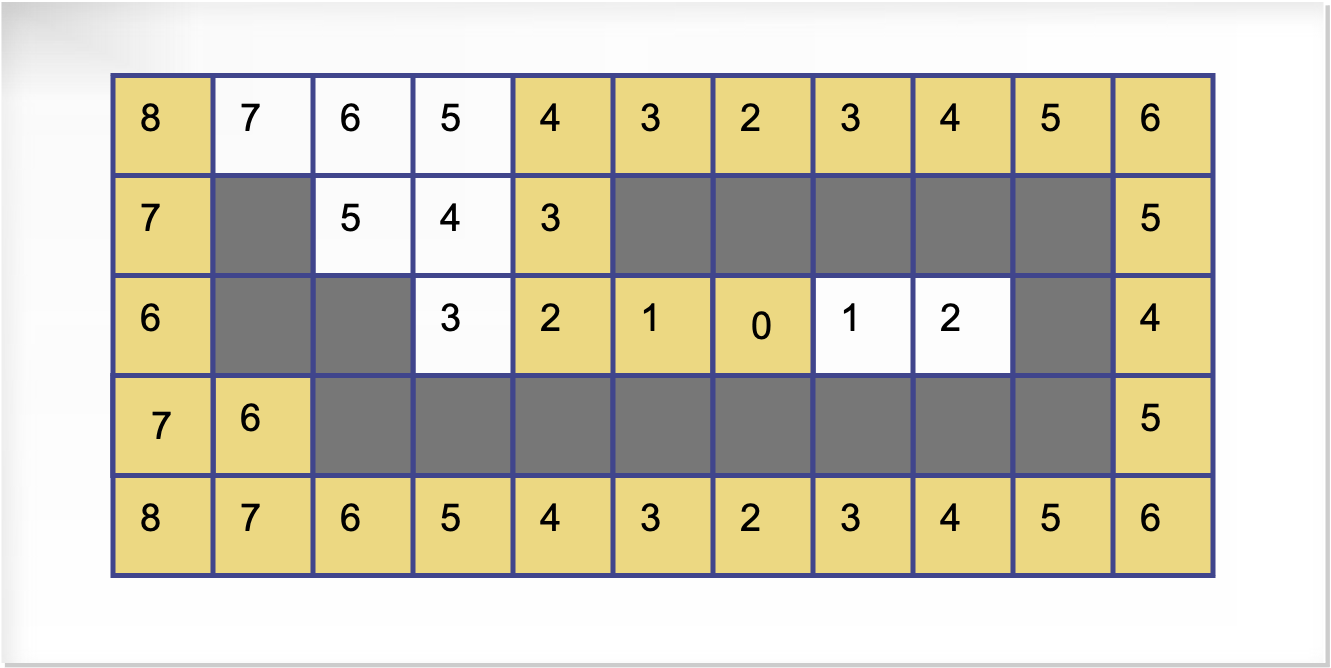
\includegraphics[scale=0.4]{./img/EjemploA3}
\end{figure}

\end{frame} 
%%%%%%%%%%%%%%%%%%%%%%%%%%%%%%%%

\begin{frame} \frametitle{Ejemplo Path Finding 4 Movimientos} \small

\begin{center}
f(N) = h(h) + g(N), con h(N) = Distancia Manhattan al objetivo
\end{center}


\begin{figure}
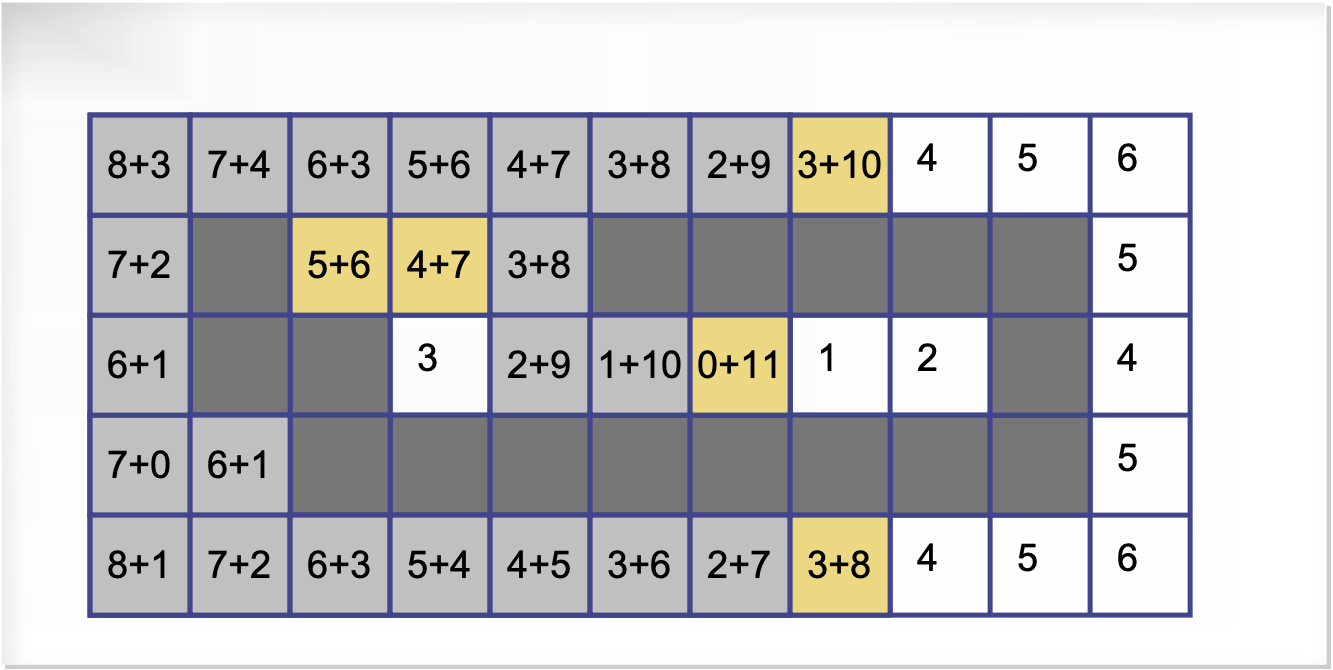
\includegraphics[scale=0.4]{./img/EjemploA4}
\end{figure}

\end{frame} 
%%%%%%%%%%%%%%%%%%%%%%%%%%%%%%%%

\begin{frame} \frametitle{Ejemplo Path Finding 8 Movimientos} \small

\begin{figure}
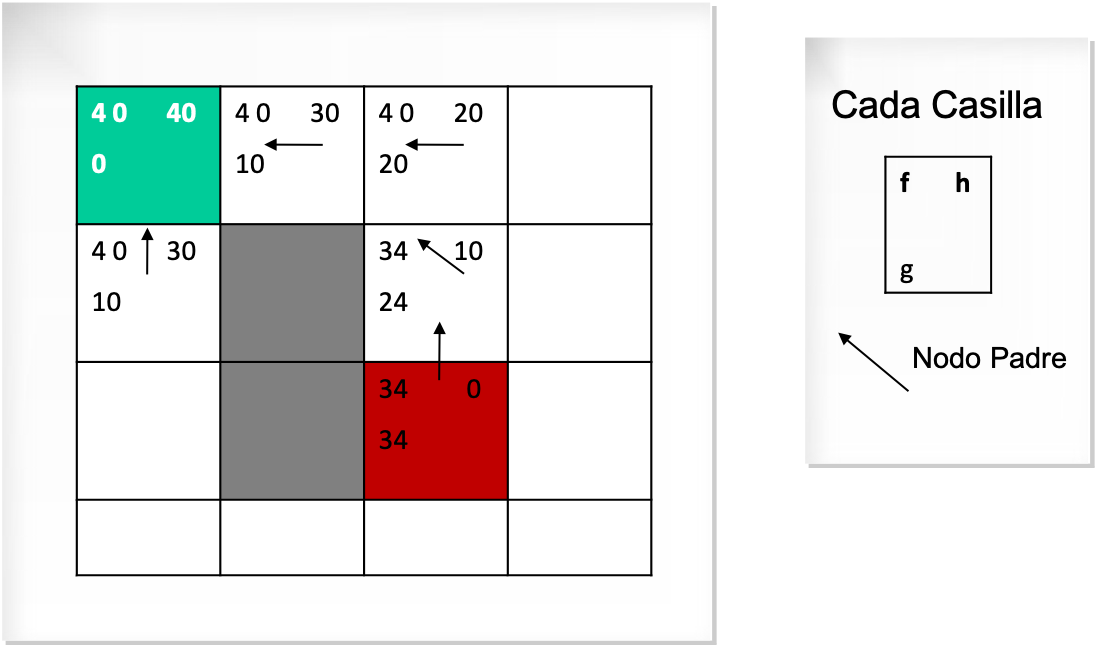
\includegraphics[scale=0.55]{./img/PathFindingEjemplo}
\end{figure}

\end{frame} 

%%%%%%%%%%%%%%%%%%%%%%%%%%%%%%%%

\begin{frame} \frametitle{Path Finding Heurísticas} \small

\begin{itemize}
\item  Distancia Manhattan:  h(n) =  (abs(n.x-goal.x) + abs(n.y-goal.y)). 
\end{itemize}


\begin{figure}
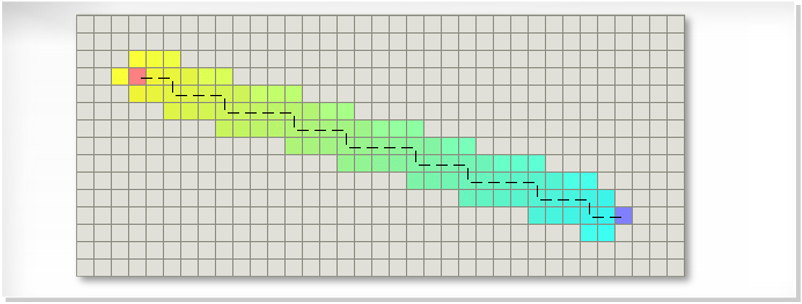
\includegraphics[scale=0.35]{./img/HManhattan}
\end{figure}

\begin{itemize}
\item  Distancia Diagonal: h(n) = max(abs(n.x-goal.x), abs(n.y-goal.y))
\end{itemize}


\begin{figure}
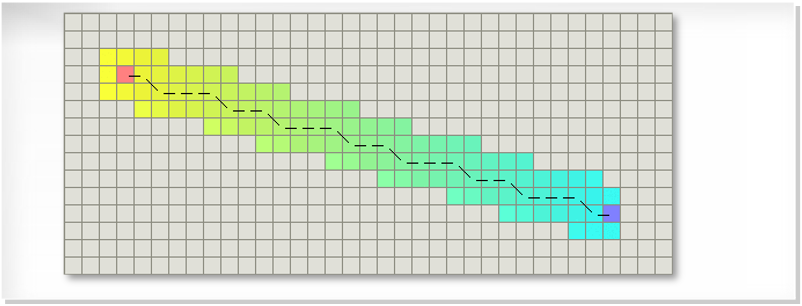
\includegraphics[scale=0.35]{./img/HDiagonal}
\end{figure}

\begin{flushright}
{\tiny Imágenes obtenidas de: \url{http://theory.stanford.edu/~amitp/GameProgramming/Heuristics.html}}
\end{flushright}

\end{frame} 

%%%%%%%%%%%%%%%%%%%%%%%%%%%%%%%%

\begin{frame} \frametitle{Path Finding Heurísticas} \small

\begin{itemize}
\item   Distancia Euclídea: h(n) = $ \sqrt{((n.x-goal.x)^2 + (n.y-goal.y)^2)}$.
\end{itemize}


\begin{figure}
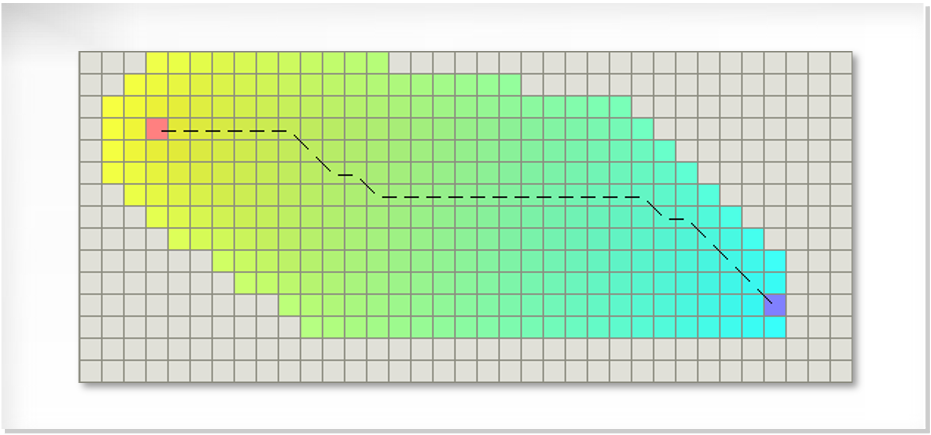
\includegraphics[scale=0.45]{./img/HEuclidea}
\end{figure}


\begin{flushright}
{\tiny Imágenes obtenidas de: \url{http://theory.stanford.edu/~amitp/GameProgramming/Heuristics.html}}
\end{flushright}

\end{frame} 


%%%%%%%%%%%%%%%%%%%%%%%%%%%%%%%%

%%%%%%%%%%%%%%%%%%%%%%%%%%%%%%%%

\begin{frame} \frametitle{PathFinding en Videojuegos} \small

Abstracción Jerárquica (Hierarchical Abstraction)
\begin{itemize}
    \item  Reduce el espacio de búsqueda que tiene que ser explorado
    \item  Realiza un cómputo del camino más rápido que A*
    \item  Algunas implementaciones:
            \begin{itemize}
                \item  HPA* (Botea, Mueller, Schaeffer 2004)
                \item  PRA* (Sturtevant, Buro 2005) 
                \item  HAA* (Harabor, Botea, 2008)
                \end{itemize}

\end{itemize}

More info: \url{https://web.archive.org/web/20190411040123/http://aigamedev.com/open/article/clearance-based-pathfinding/} 

\end{frame} 

%%%%%%%%%%%%%%%%%%%%%%%%%%%%%%%%
%%%%%%%%%%%%%%%%%%%%%%%%%%%%%%%%
%%%%%%%%%%%%%%%%%%%%%%%%%%%%%%%%

\begin{chapter}[images/etsiinformatica4.png]{uicblue}{Búsqueda multiagente}
\end{chapter}

\section{Búsqueda multiagente}

%%%%%%%%%%%%%%%%%%%%%%%%%%%%%%%%

\begin{frame} \frametitle{Búsqueda multiagente} \small

\begin{itemize}
    \item  Entornos multiagente, donde cada agente debe considerar las acciones de los otros agentes. 
     \item  Juegos: Entornos competitivos donde los objetivos del agente están en conflicto, dan lugar a problemas de búsqueda entre adversarios.
      \begin{itemize}
        \item Ajedrez, Otelo, Backgammon, Go
        \item Ajedrez: Árbol de búsqueda tiene $10^{154}$ nodos.
        \end{itemize}

\item   Capacidad de tomar decisión cuando no es factible calcular la decisión óptima. 

        \begin{itemize}
        \item \textbf{Poda}: Nos permiten ignorar partes del árbol búsqueda.
        \item \textbf{Funciones evaluación}: Heurísticas que permiten aproximar la utilidad sin hacer búsqueda completa.
        \end{itemize}


\end{itemize}


\end{frame} 

%%%%%%%%%%%%%%%%%%%%%%%%%%%%%%%%

\begin{frame} \frametitle{Elementos Búsqueda multiagente} \small

\begin{itemize}
    \item  \textbf{Estado Inicial}: Posición tablero y jugador que mueve
    \item  \textbf{Función sucesor}: Lista pares (movimiento, estado) , estado resultante.
    \item  \textbf{Test terminal}: Cuando finaliza el juego. Estados terminales.
    \item  \textbf{Función Utilidad}: Valor numérico a los estados terminales.
Por ejemplo (suma nula): Triunfo +1, Pérdida -1, Empate 0 
   \item \textbf{Árbol del juego}: Definido mediante estado inicial y los movimientos legales.

\end{itemize}

\end{frame} 

%%%%%%%%%%%%%%%%%%%%%%%%%%%%%%%%
%%%%%%%%%%%%%%%%%%%%%%%%%%%%%%%%

\begin{chapter}[images/etsiinformatica4.png]{uicblue}{Búsqueda multiagente \\ 
Algoritmo Minimax}
\end{chapter}

\subsection{Algoritmo Minimax}

%%%%%%%%%%%%%%%%%%%%%%%%%%%%%%%%

\begin{frame} \frametitle{Algoritmo Minimax} \small

\begin{itemize}
    \item  Juegos 2 jugadores (MAX y MIN). Primero mueve MAX y luego MIN por turnos hasta que termina
    \item  Árbol del juego del Tres en Raya:
\end{itemize}

\begin{figure}
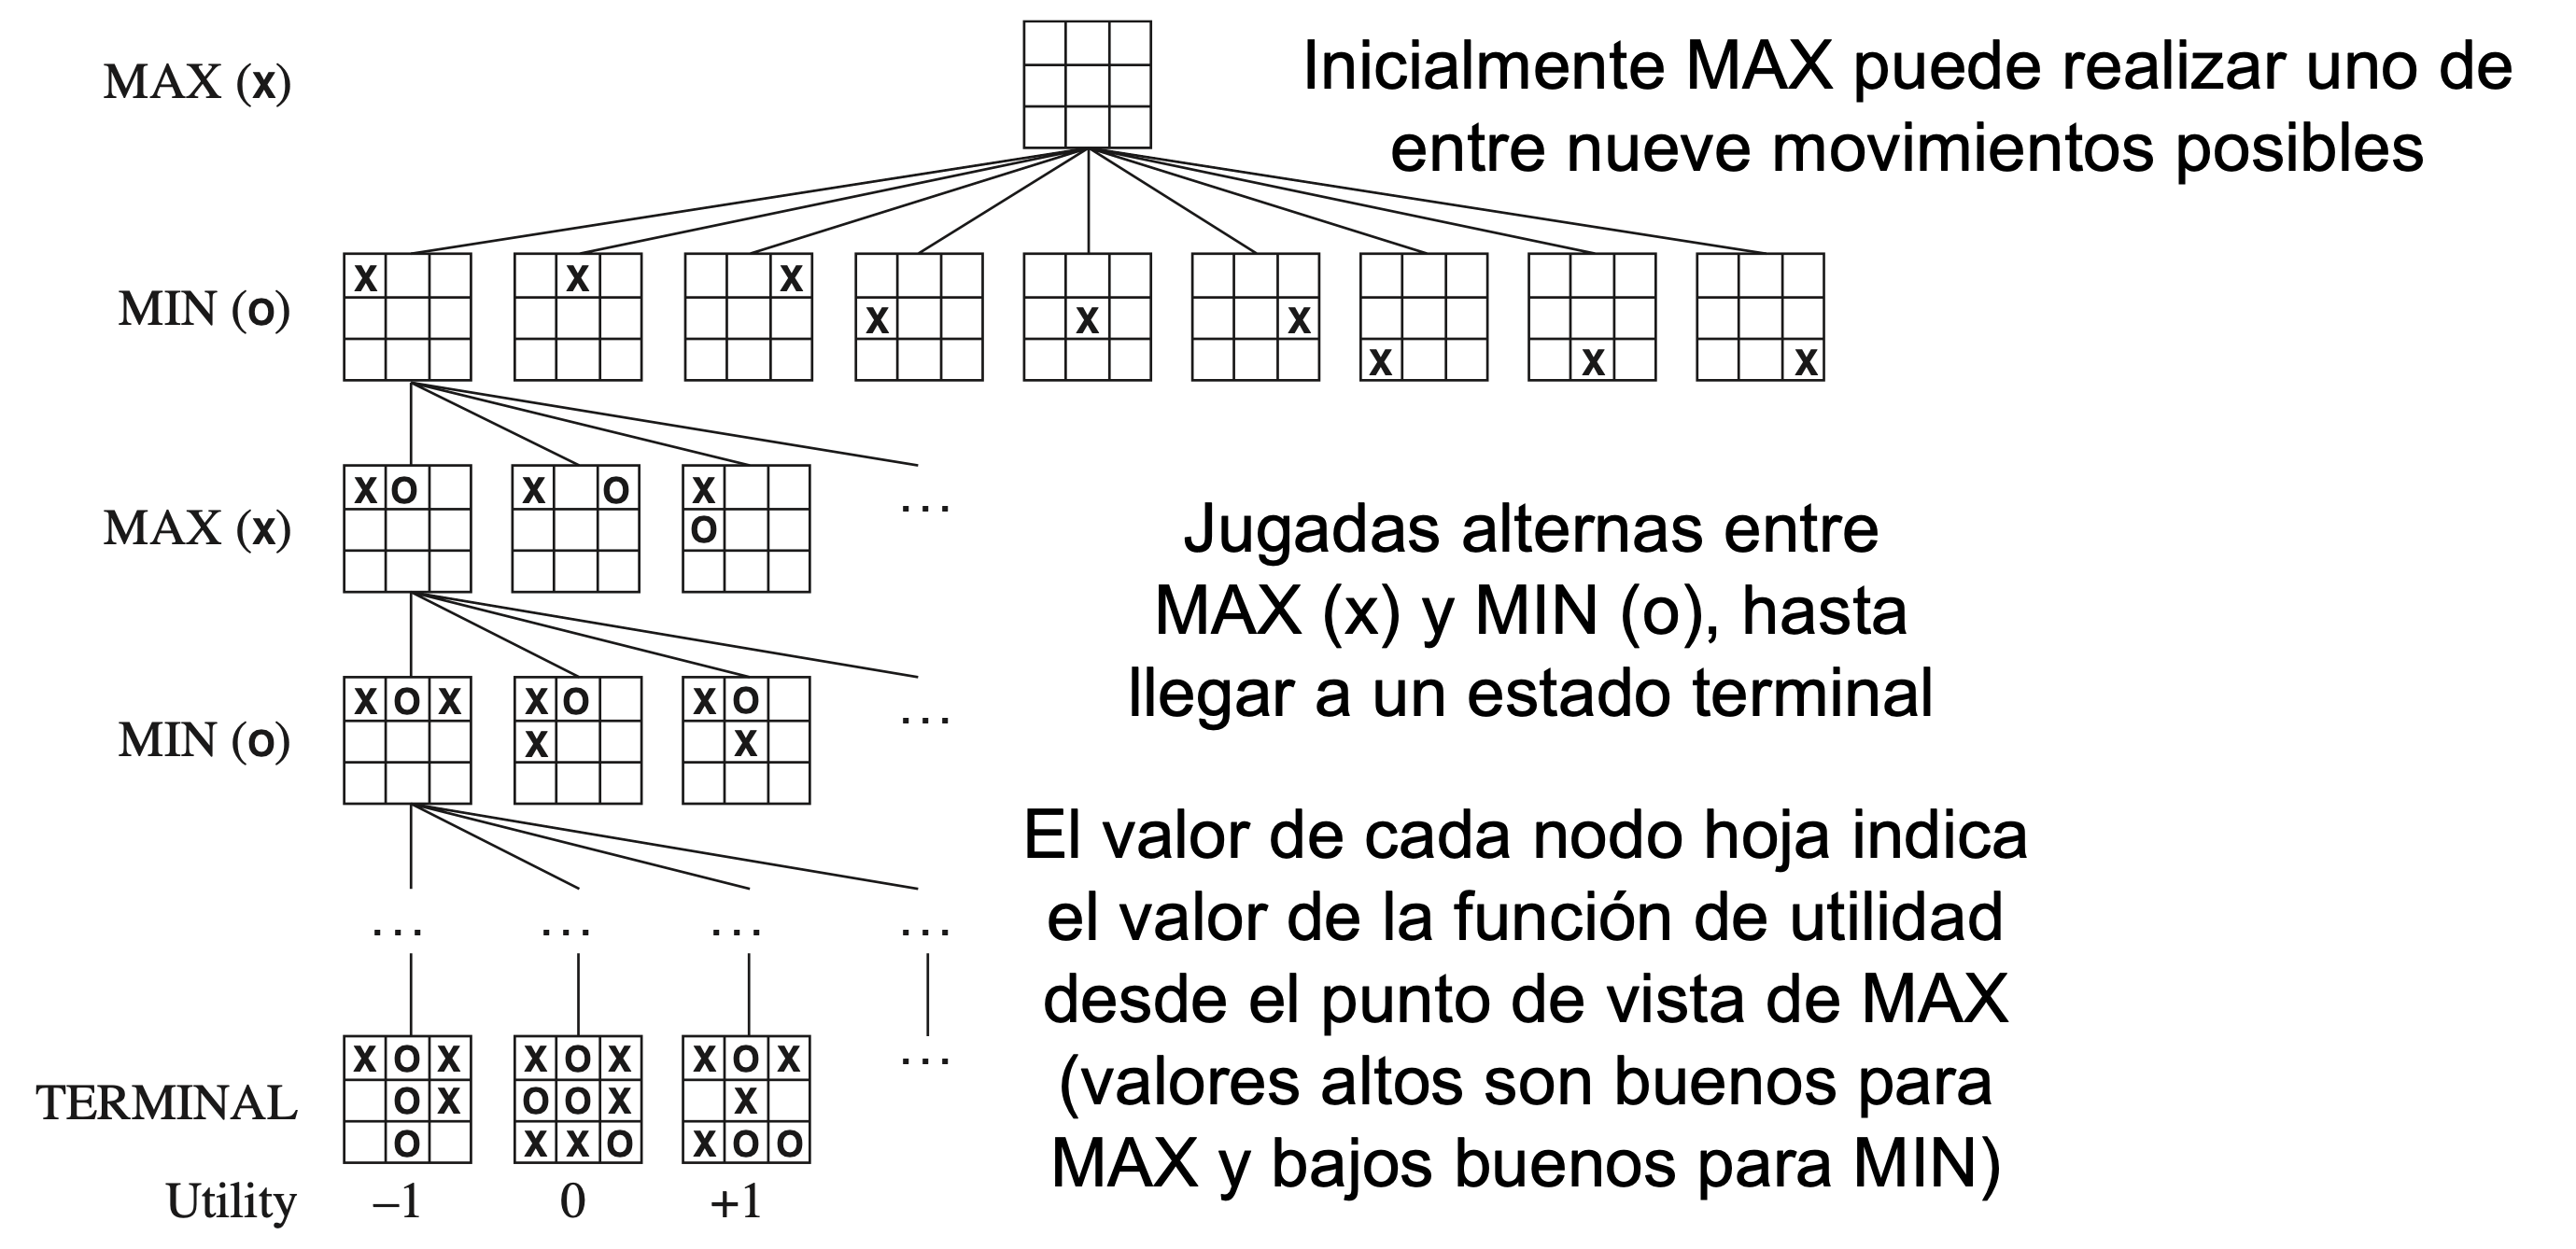
\includegraphics[scale=0.4]{./img/TresRayaMinMax}
\end{figure}


\end{frame} 

%%%%%%%%%%%%%%%%%%%%%%%%%%%%%%%%

\begin{frame} \frametitle{Algoritmo Minimax} \small

\begin{enumerate}
    \item  Tiene por objetivo decidir un movimiento para MAX.
    \item  Hipótesis:

    \begin{itemize}
    \item  Jugador MAX trata de maximizar su beneficio (función de utilidad).
    \item  Jugador MIN trata de minimizar su pérdida.
    \item  Suponemos Jugadores juegan de forma óptima.
    \end{itemize}

\item  Aplicación algoritmo:
\begin{enumerate}
    \item Generar árbol entero hasta nodos terminales
    \item Aplicar función utilidad a nodos terminales
    \item Propagar hacia arriba para generar nuevos valores de utilidad para todos los nodos\\
     minimizando para MIN\\
     maximizando para MAX\\
    \item Elección jugada con máximo valor de utilidad
\end{enumerate}

\end{enumerate}

\end{frame} 

%%%%%%%%%%%%%%%%%%%%%%%%%%%%%%%%

\begin{frame} \frametitle{Algoritmo Minimax} \small

\begin{figure}
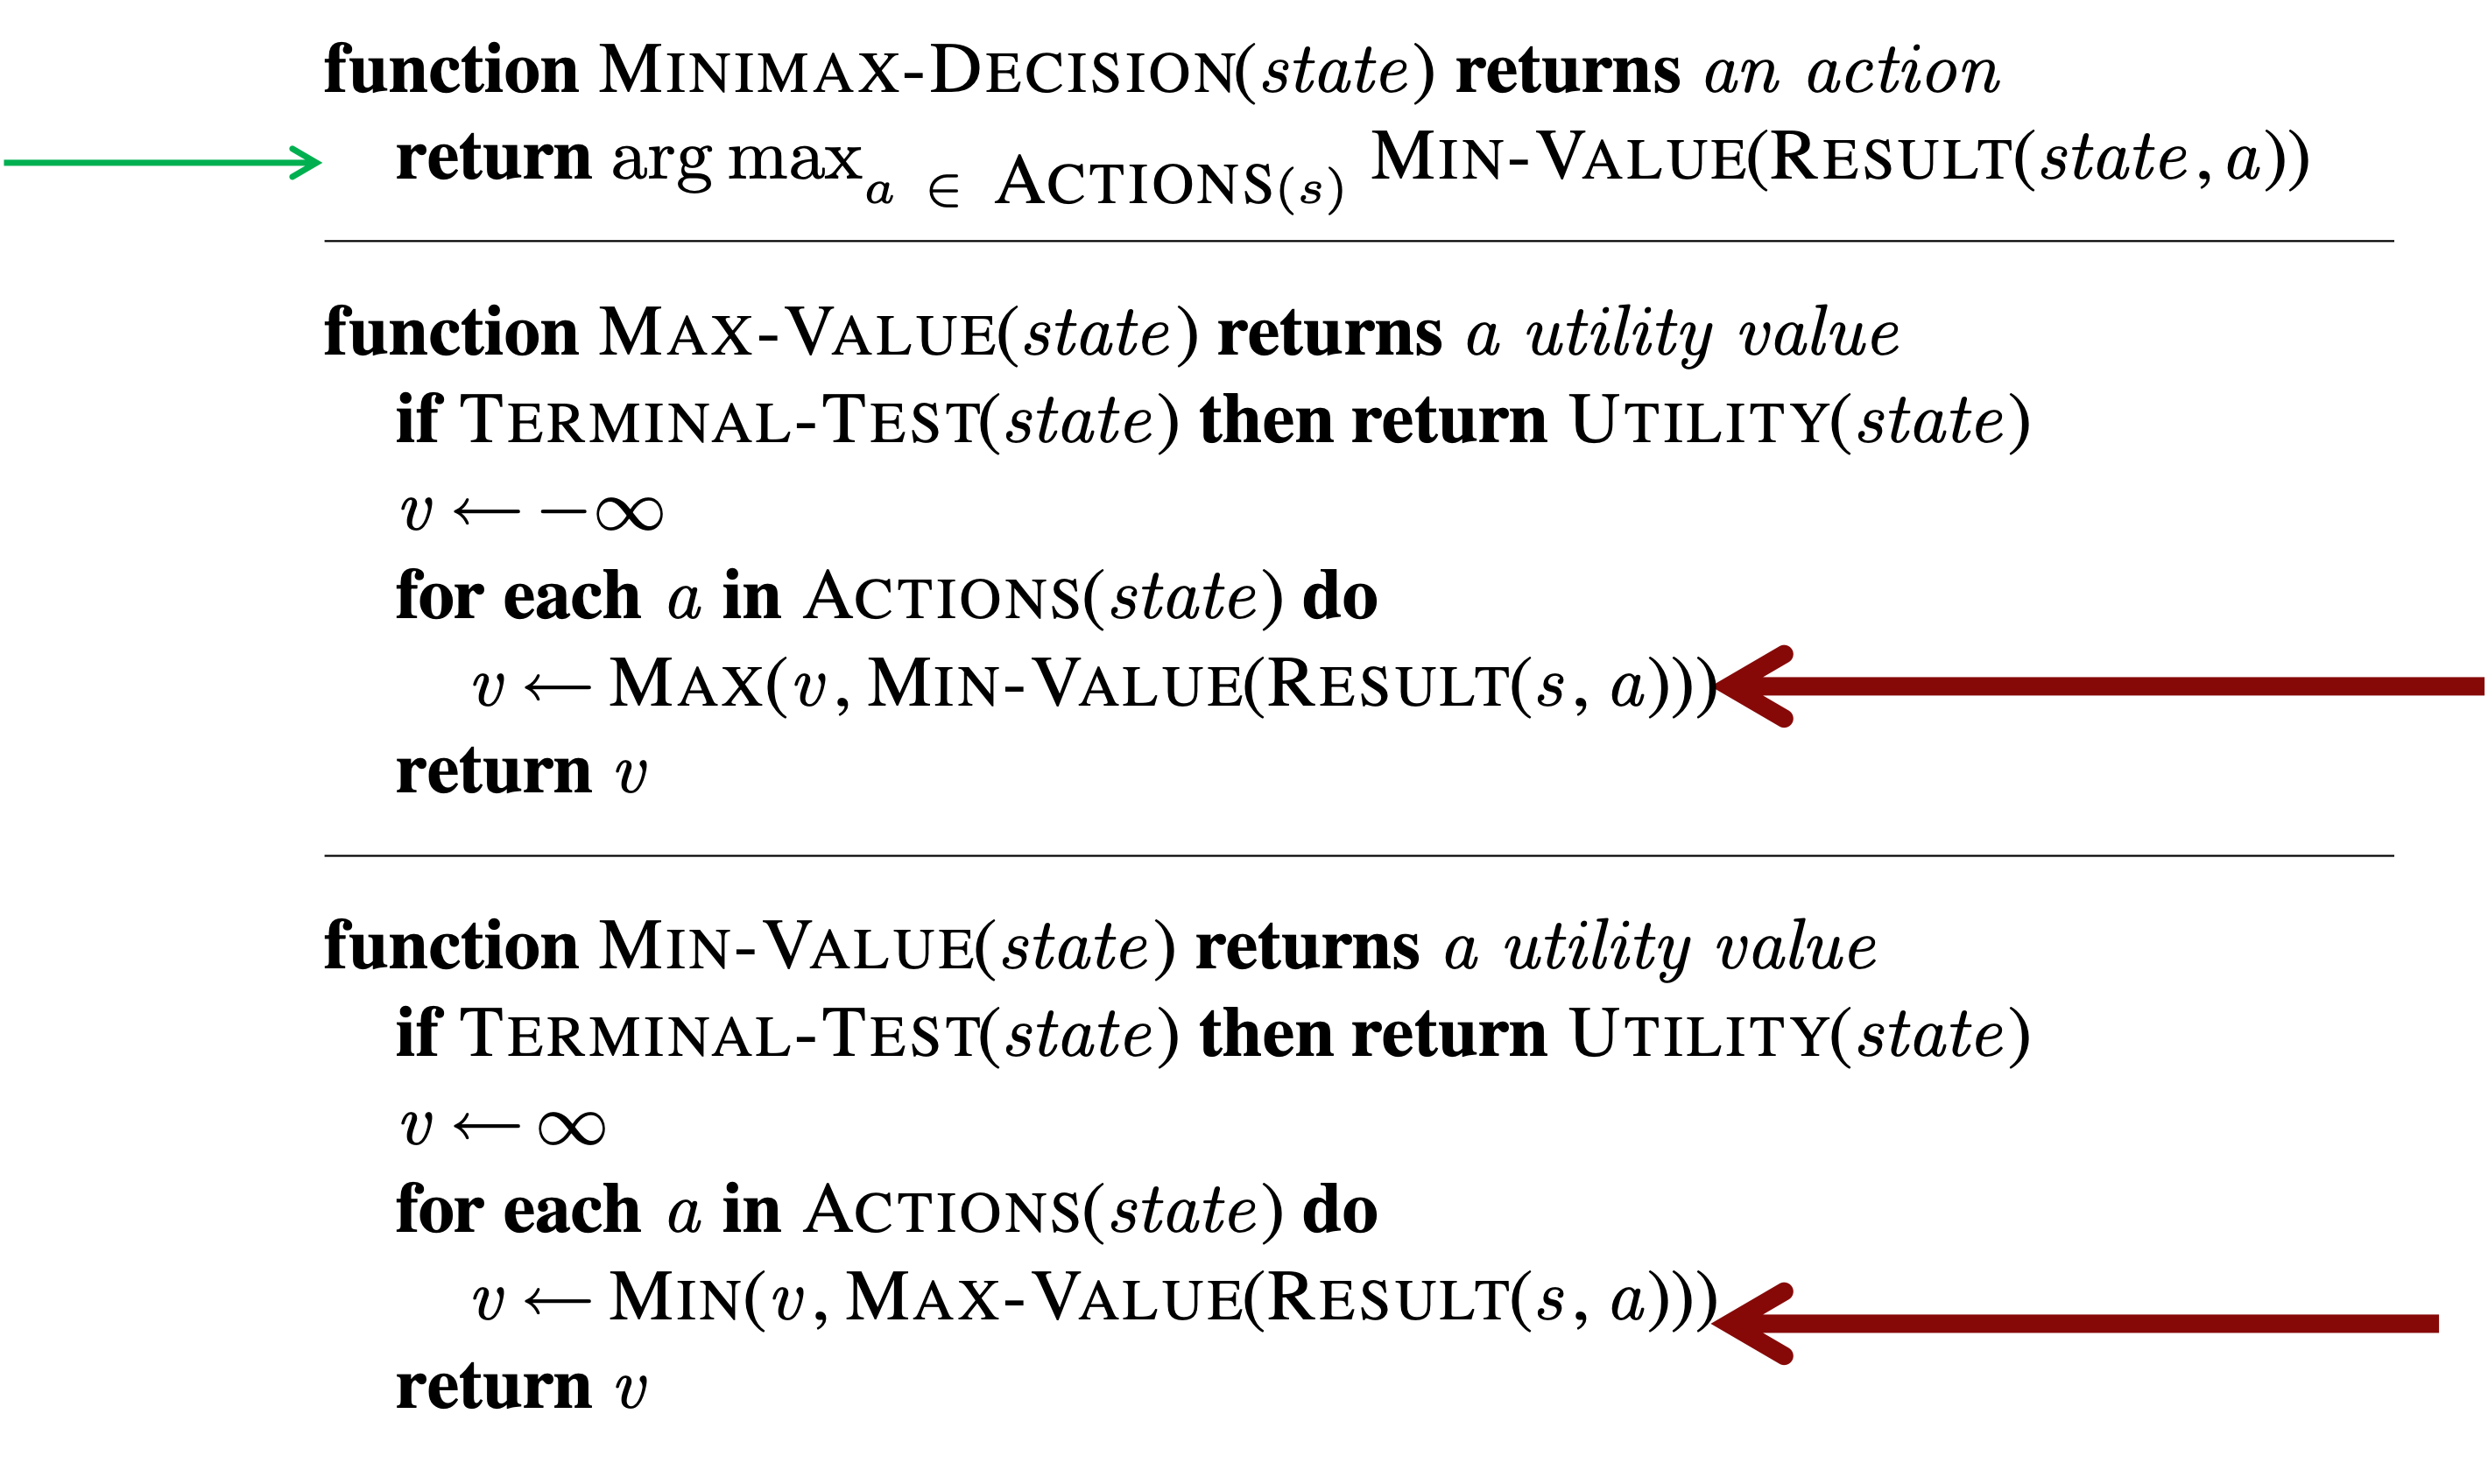
\includegraphics[scale=0.47]{./img/AlgoritmoMinimax}
\end{figure}

\end{frame} 

%%%%%%%%%%%%%%%%%%%%%%%%%%%%%%%%

\begin{frame} \frametitle{Algoritmo Minimax Ed. 4} \small

\begin{figure}
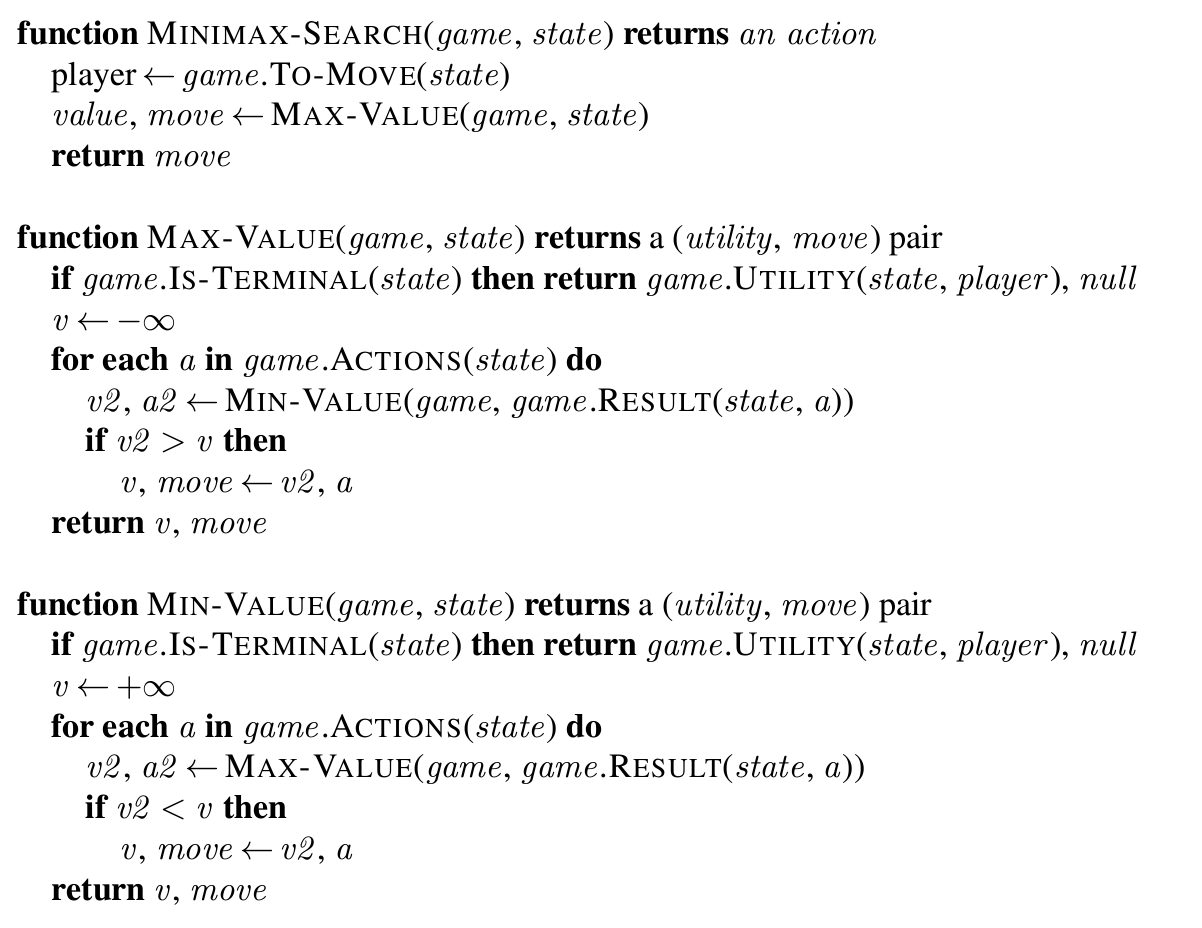
\includegraphics[scale=0.35]{./img/MinimaxNew}
\end{figure}

\end{frame} 

%%%%%%%%%%%%%%%%%%%%%%%%%%%%%%%%

\begin{frame} \frametitle{Algoritmo Minimax} \small

\begin{figure}
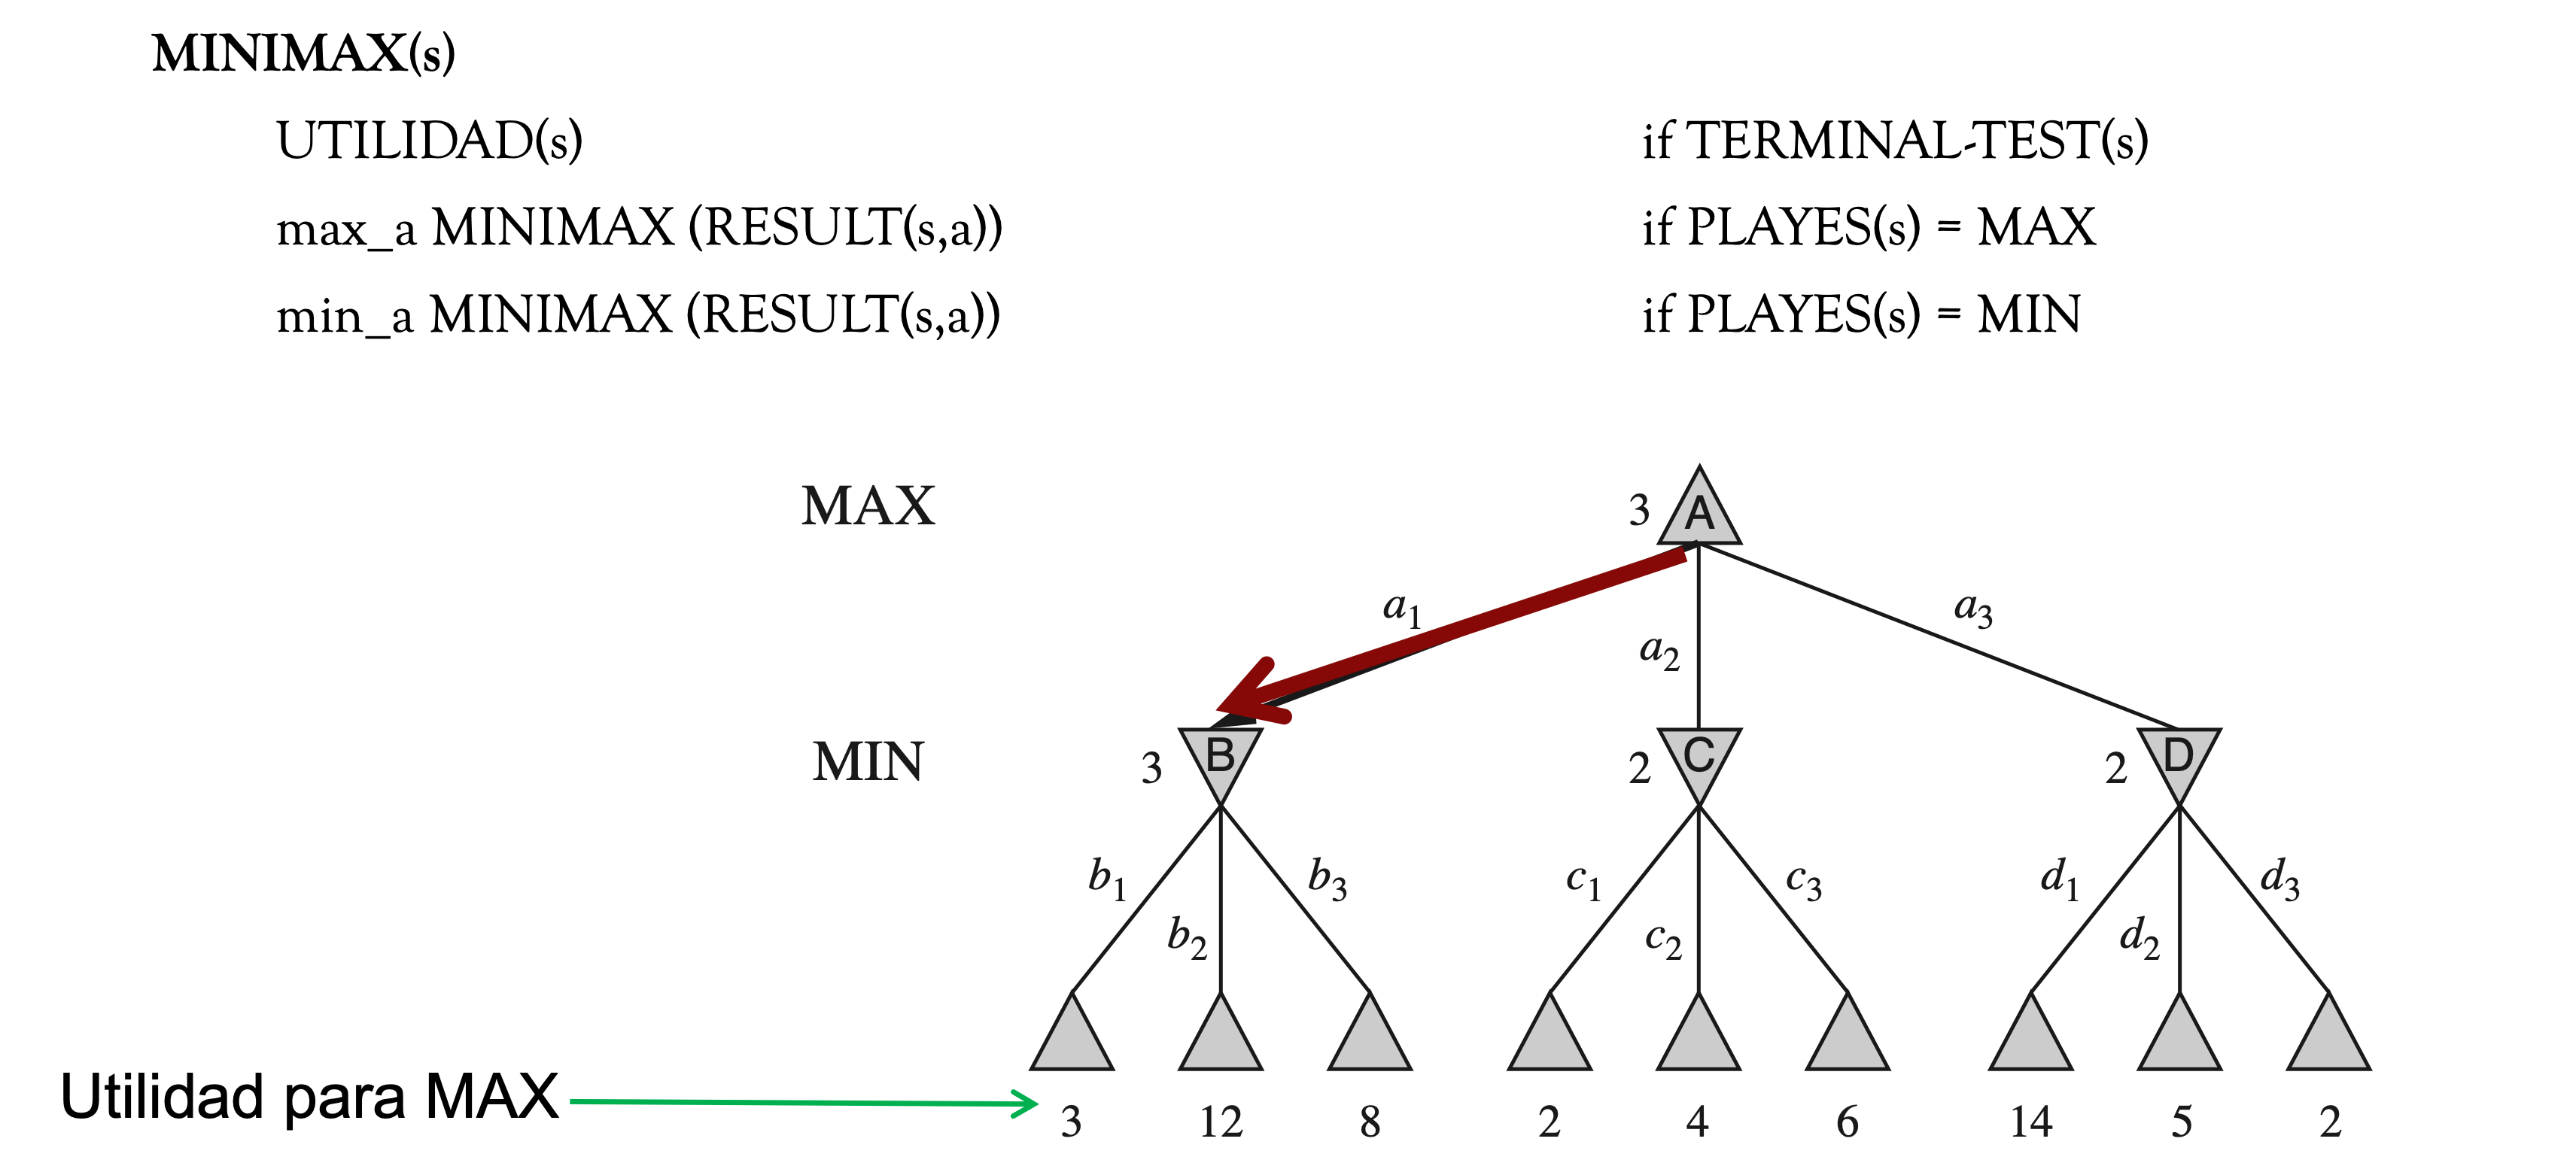
\includegraphics[scale=0.47]{./img/Minimax2}
\end{figure}

\end{frame} 


%%%%%%%%%%%%%%%%%%%%%%%%%%%%%%%%

\begin{frame} \frametitle{Ejemplo 1 } \small

\begin{figure}
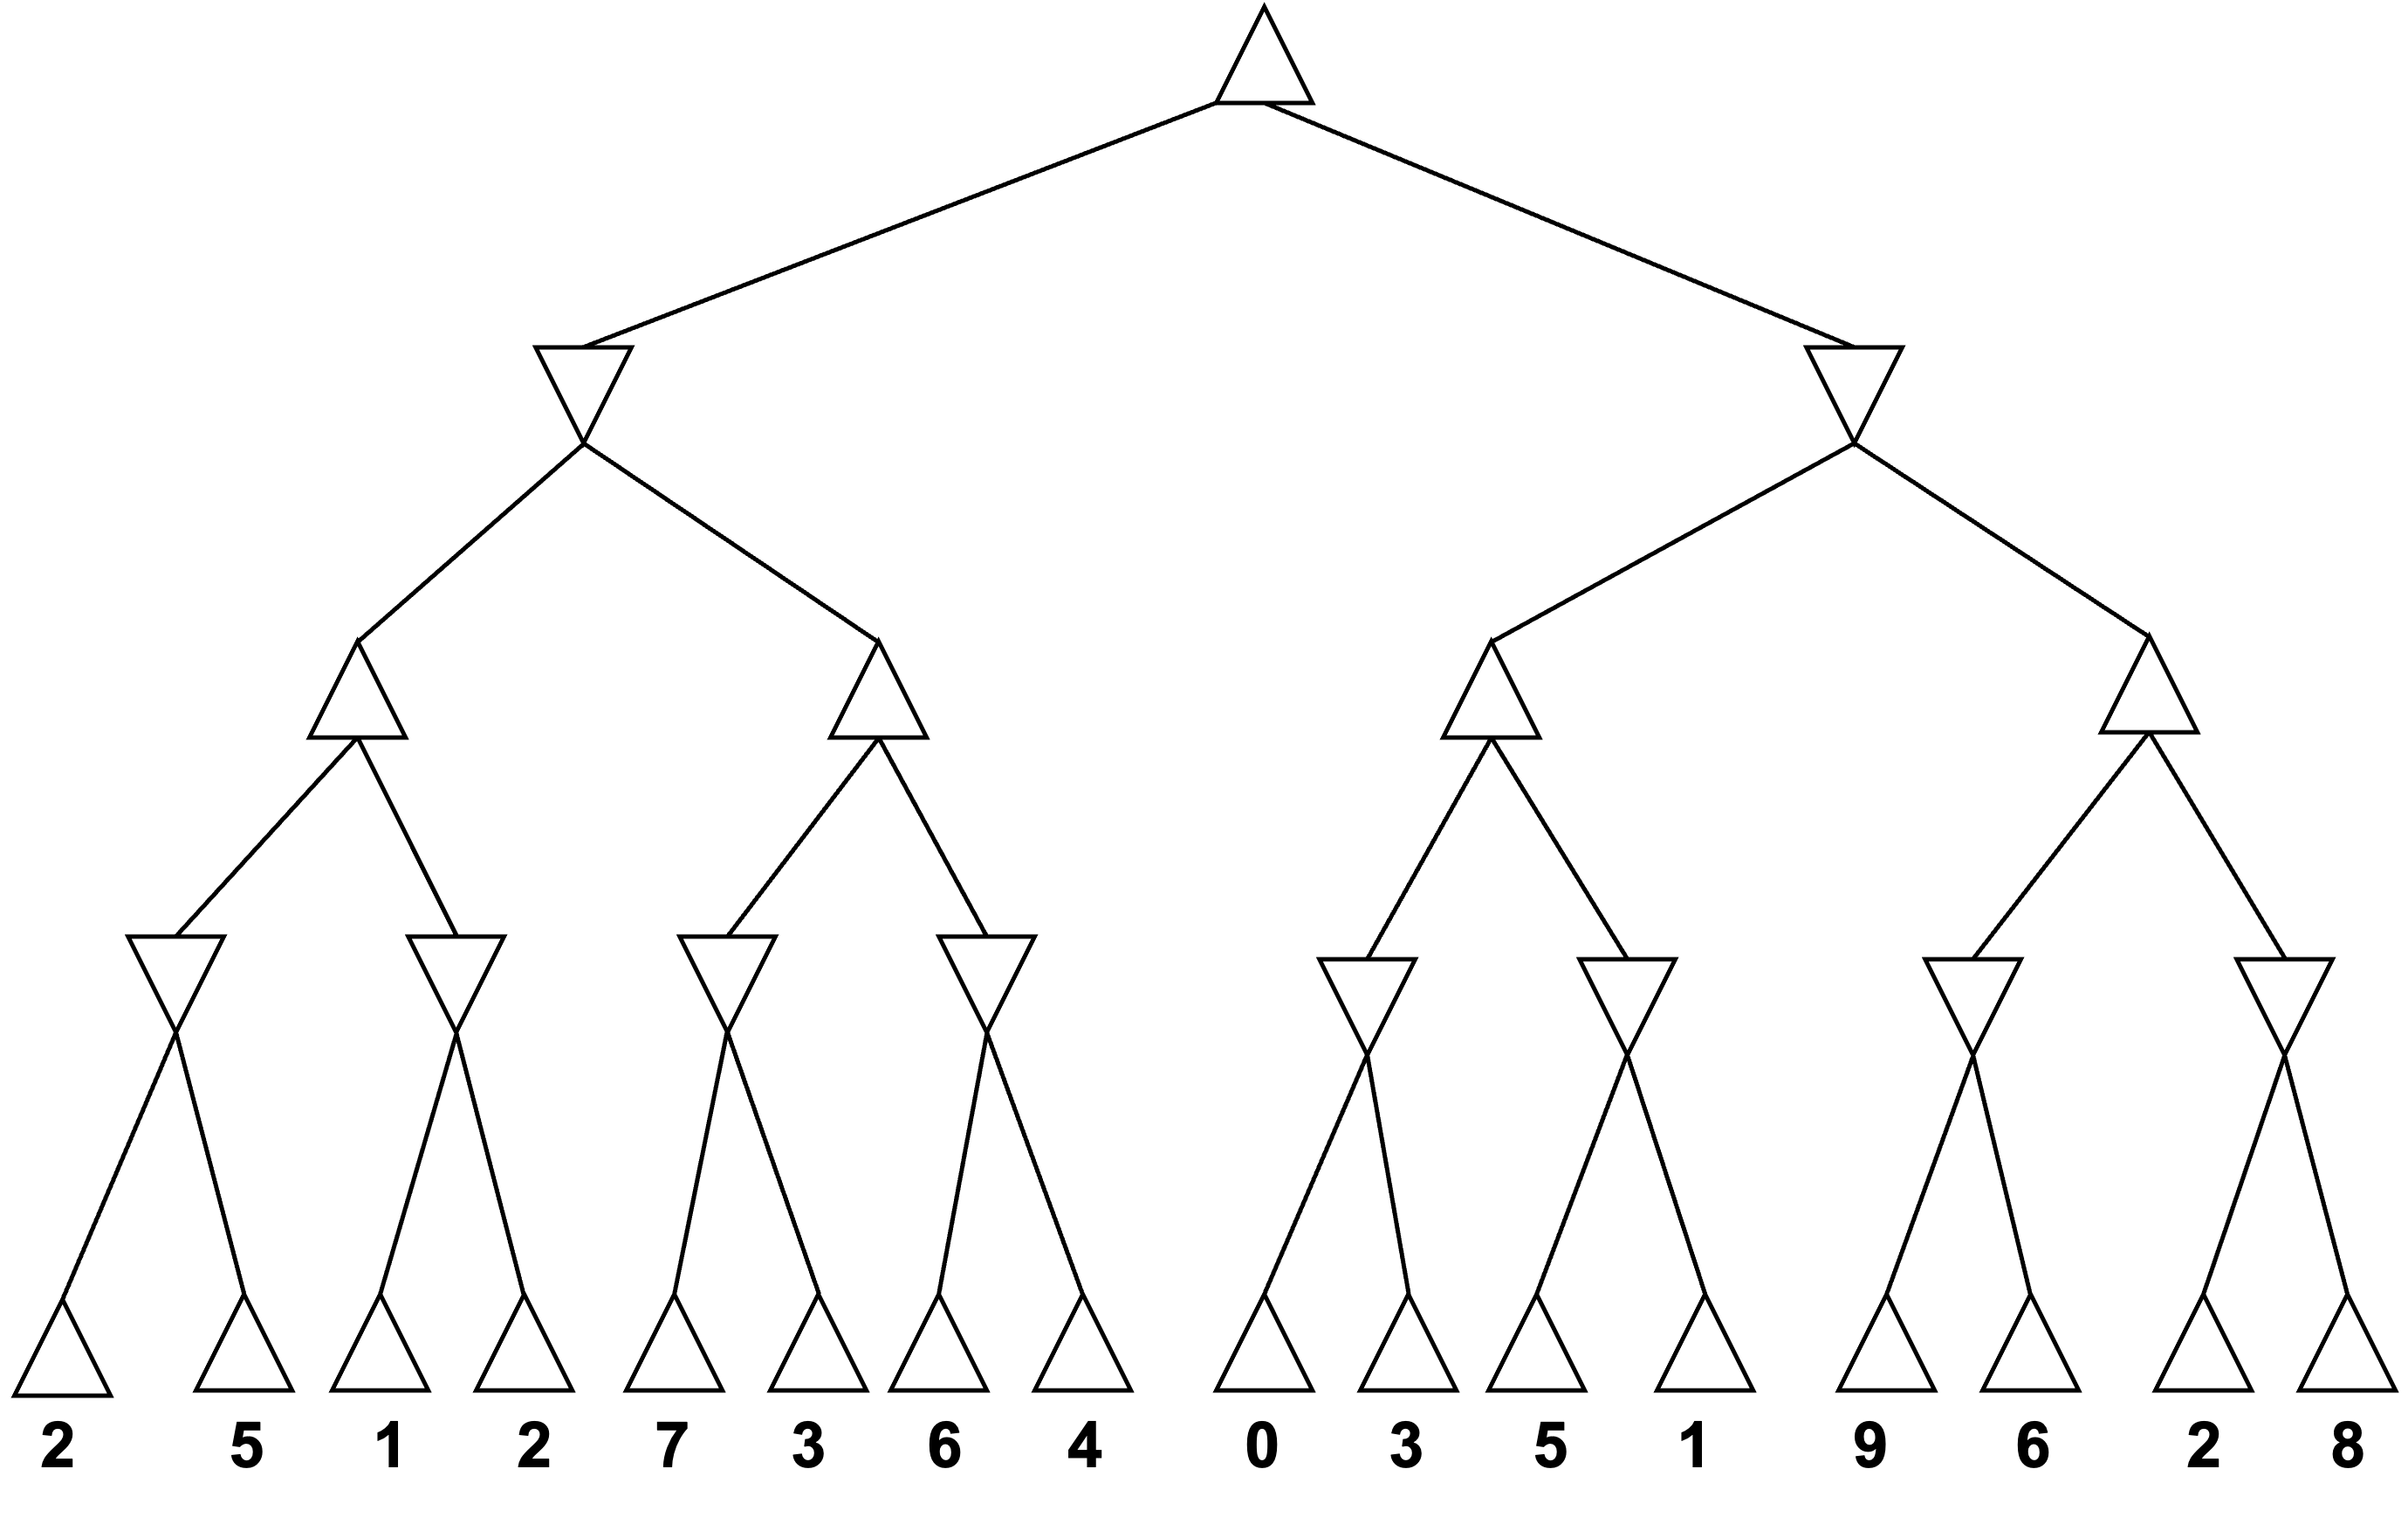
\includegraphics[scale=0.45]{./img/Ejemplo1}
\end{figure}

\end{frame} 

%%%%%%%%%%%%%%%%%%%%%%%%%%%%%%%%

\begin{frame} \frametitle{Ejemplo 1 } \small

\begin{figure}
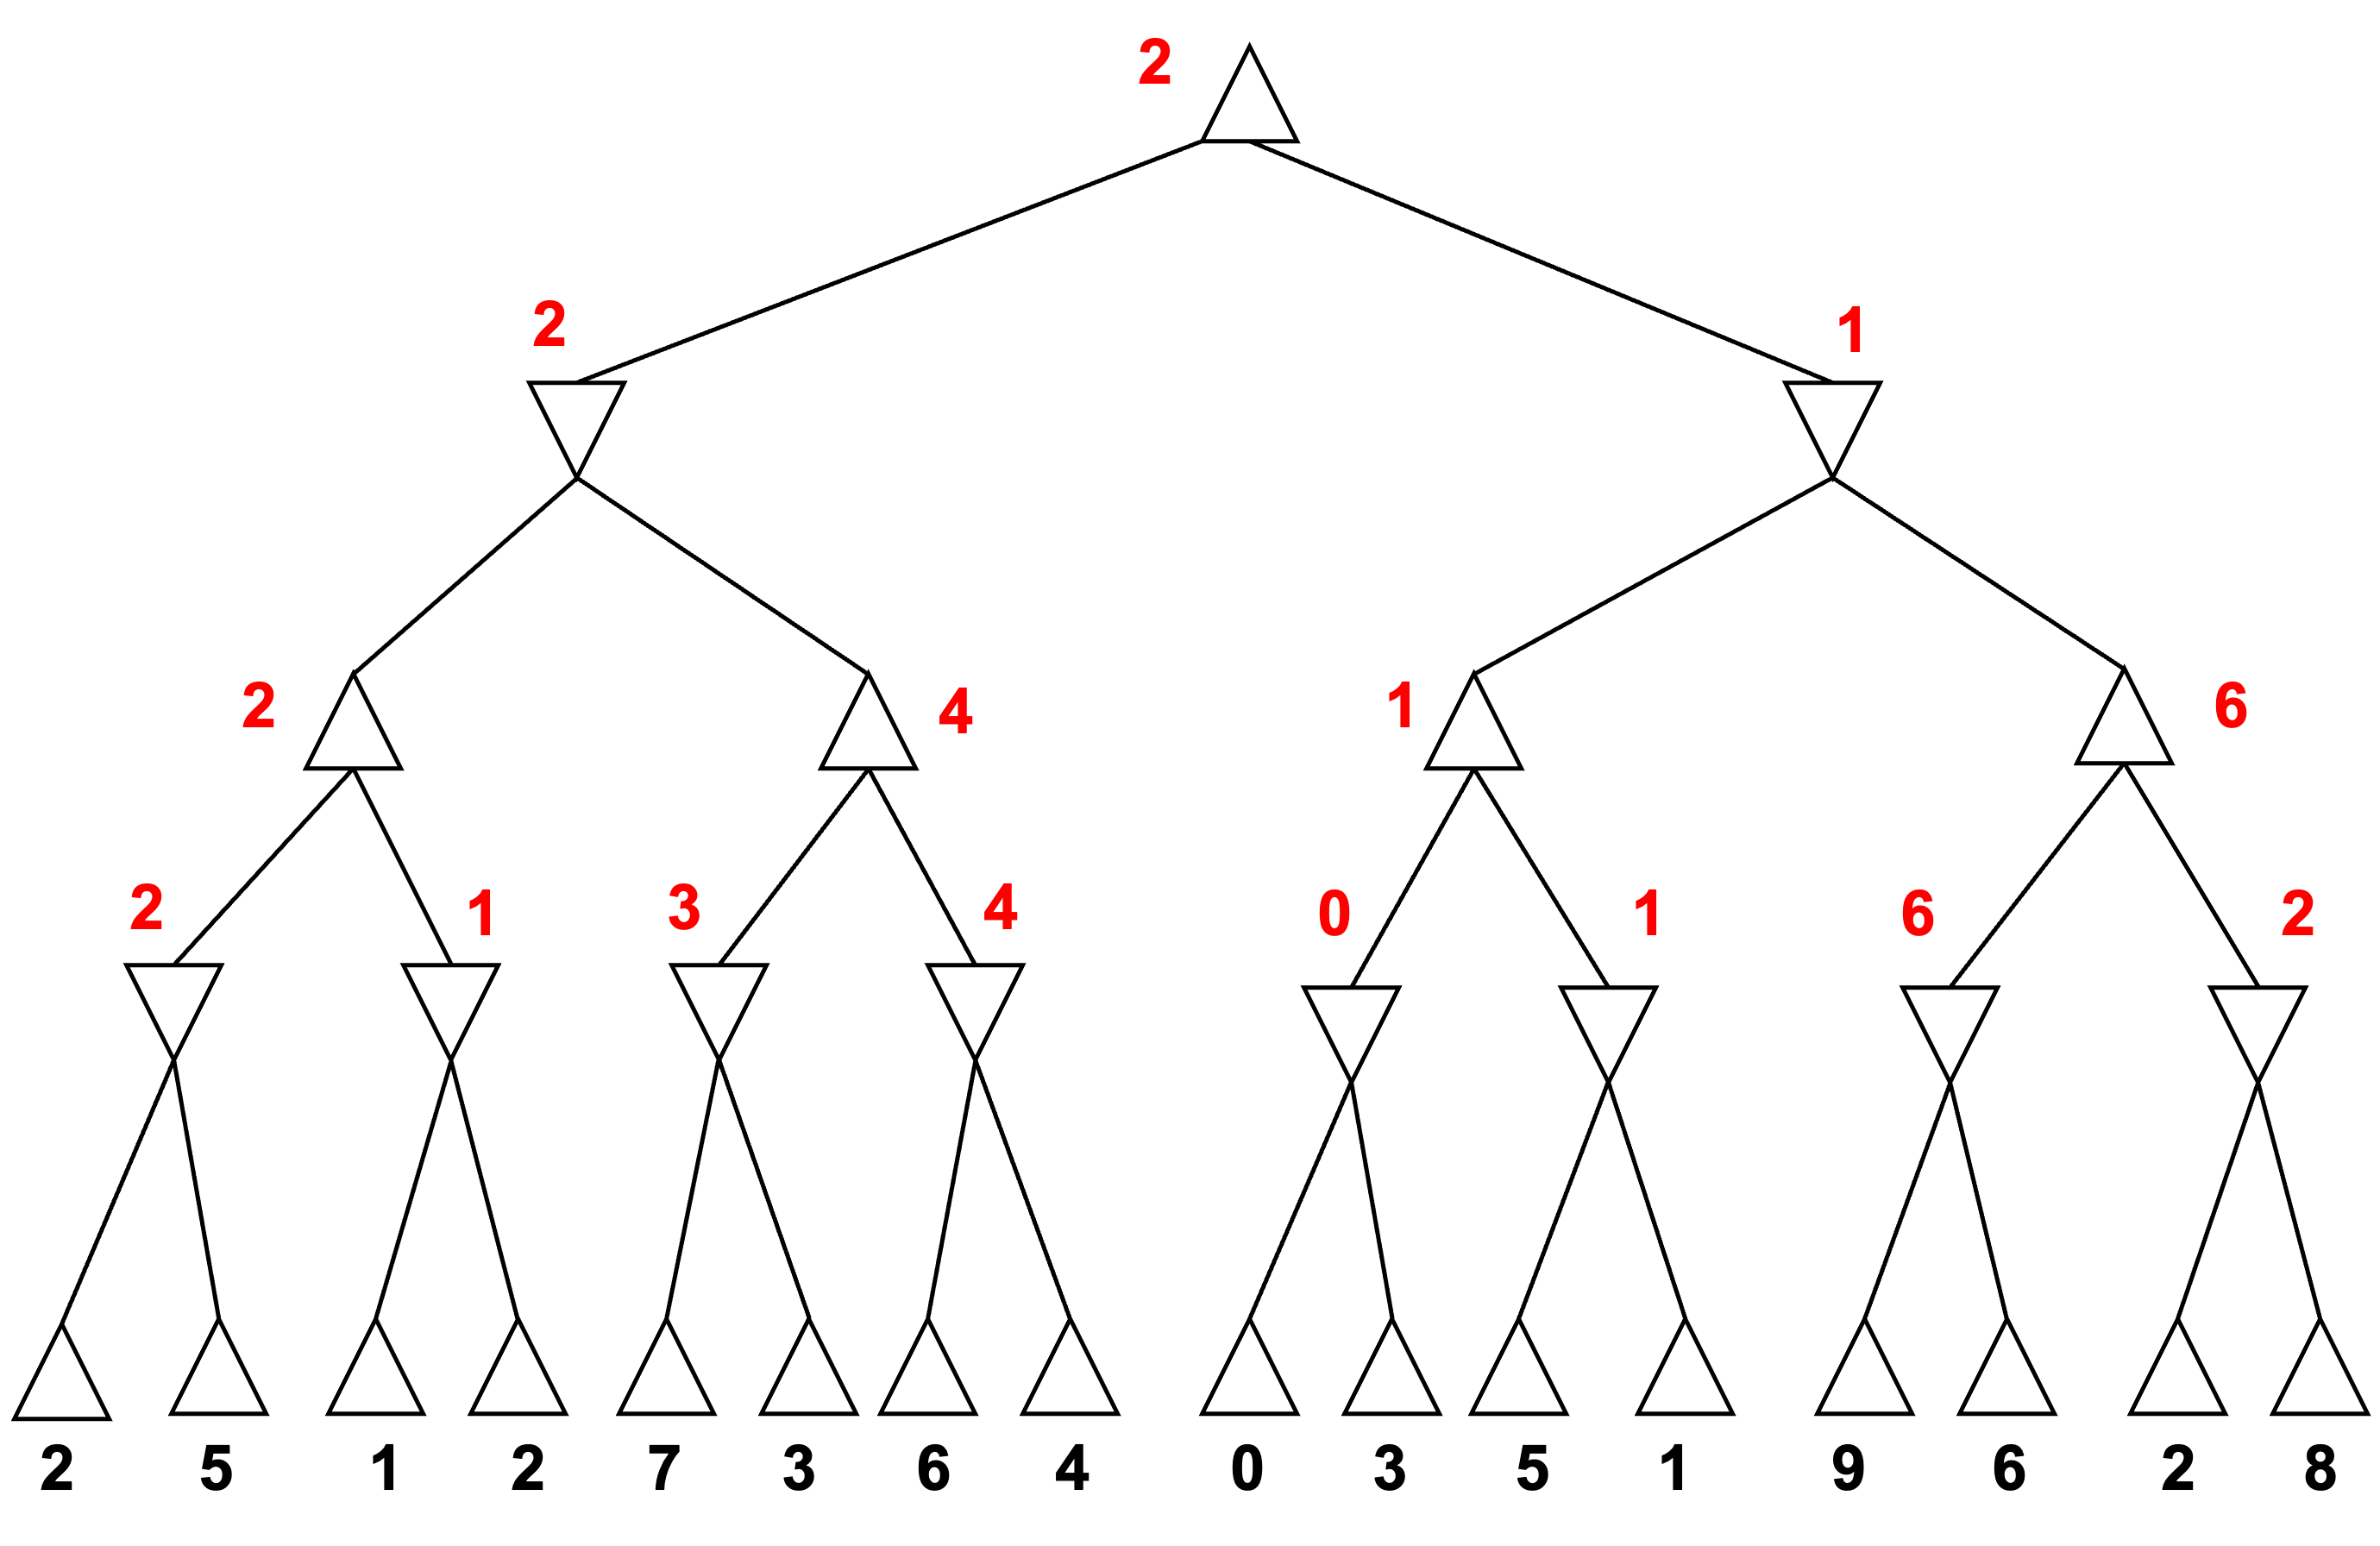
\includegraphics[scale=0.45]{./img/Ejemplo1Sol}
\end{figure}

\end{frame} 

%%%%%%%%%%%%%%%%%%%%%%%%%%%%%%%%
%%%%%%%%%%%%%%%%%%%%%%%%%%%%%%%%

\begin{chapter}[images/etsiinformatica4.png]{uicblue}{Búsqueda multiagente \\ 
Poda Alfa-Beta}
\end{chapter}

\subsection{Poda Alfa-Beta}

%%%%%%%%%%%%%%%%%%%%%%%%%%%%%%%%

\begin{frame} \frametitle{Poda $\alpha$-$\beta$ } \small


\begin{itemize}
    \item No afecta al resultado final
    \item Su efectividad depende del orden en que se consideren los movimientos
    \item $\alpha$ valor de la mejor elección para MAX (valor más alto) que hemos encontrado en el camino hasta ahora
    \item $\beta$  valor de la mejor elección para MIN (valor más bajo) que hemos encontrado en el camino hasta ahora
\end{itemize}
\end{frame} 

%%%%%%%%%%%%%%%%%%%%%%%%%%%%%%%%

\begin{frame} \frametitle{Poda $\alpha$-$\beta$ } \small

\begin{figure}
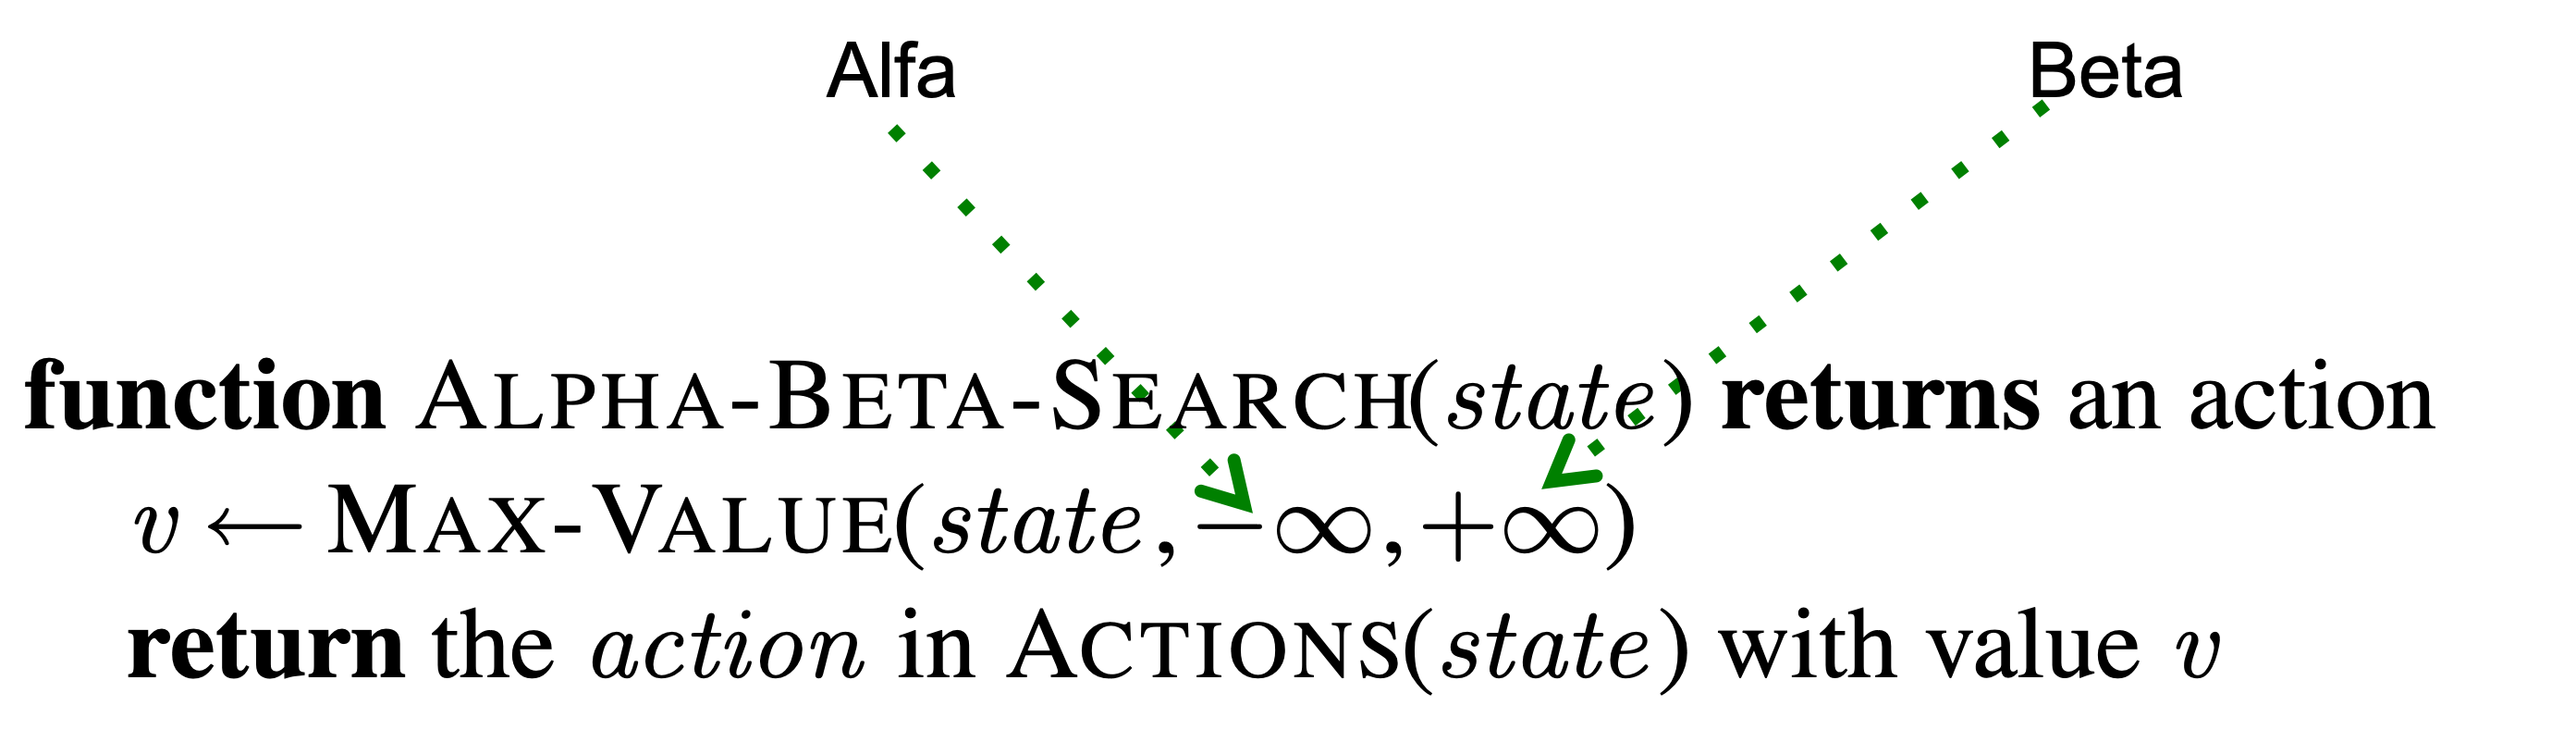
\includegraphics[scale=0.6]{./img/alfabeta1}
\end{figure}
\end{frame} 

%%%%%%%%%%%%%%%%%%%%%%%%%%%%%%%%

\begin{frame} \frametitle{Poda $\alpha$-$\beta$ } \small

\begin{figure}
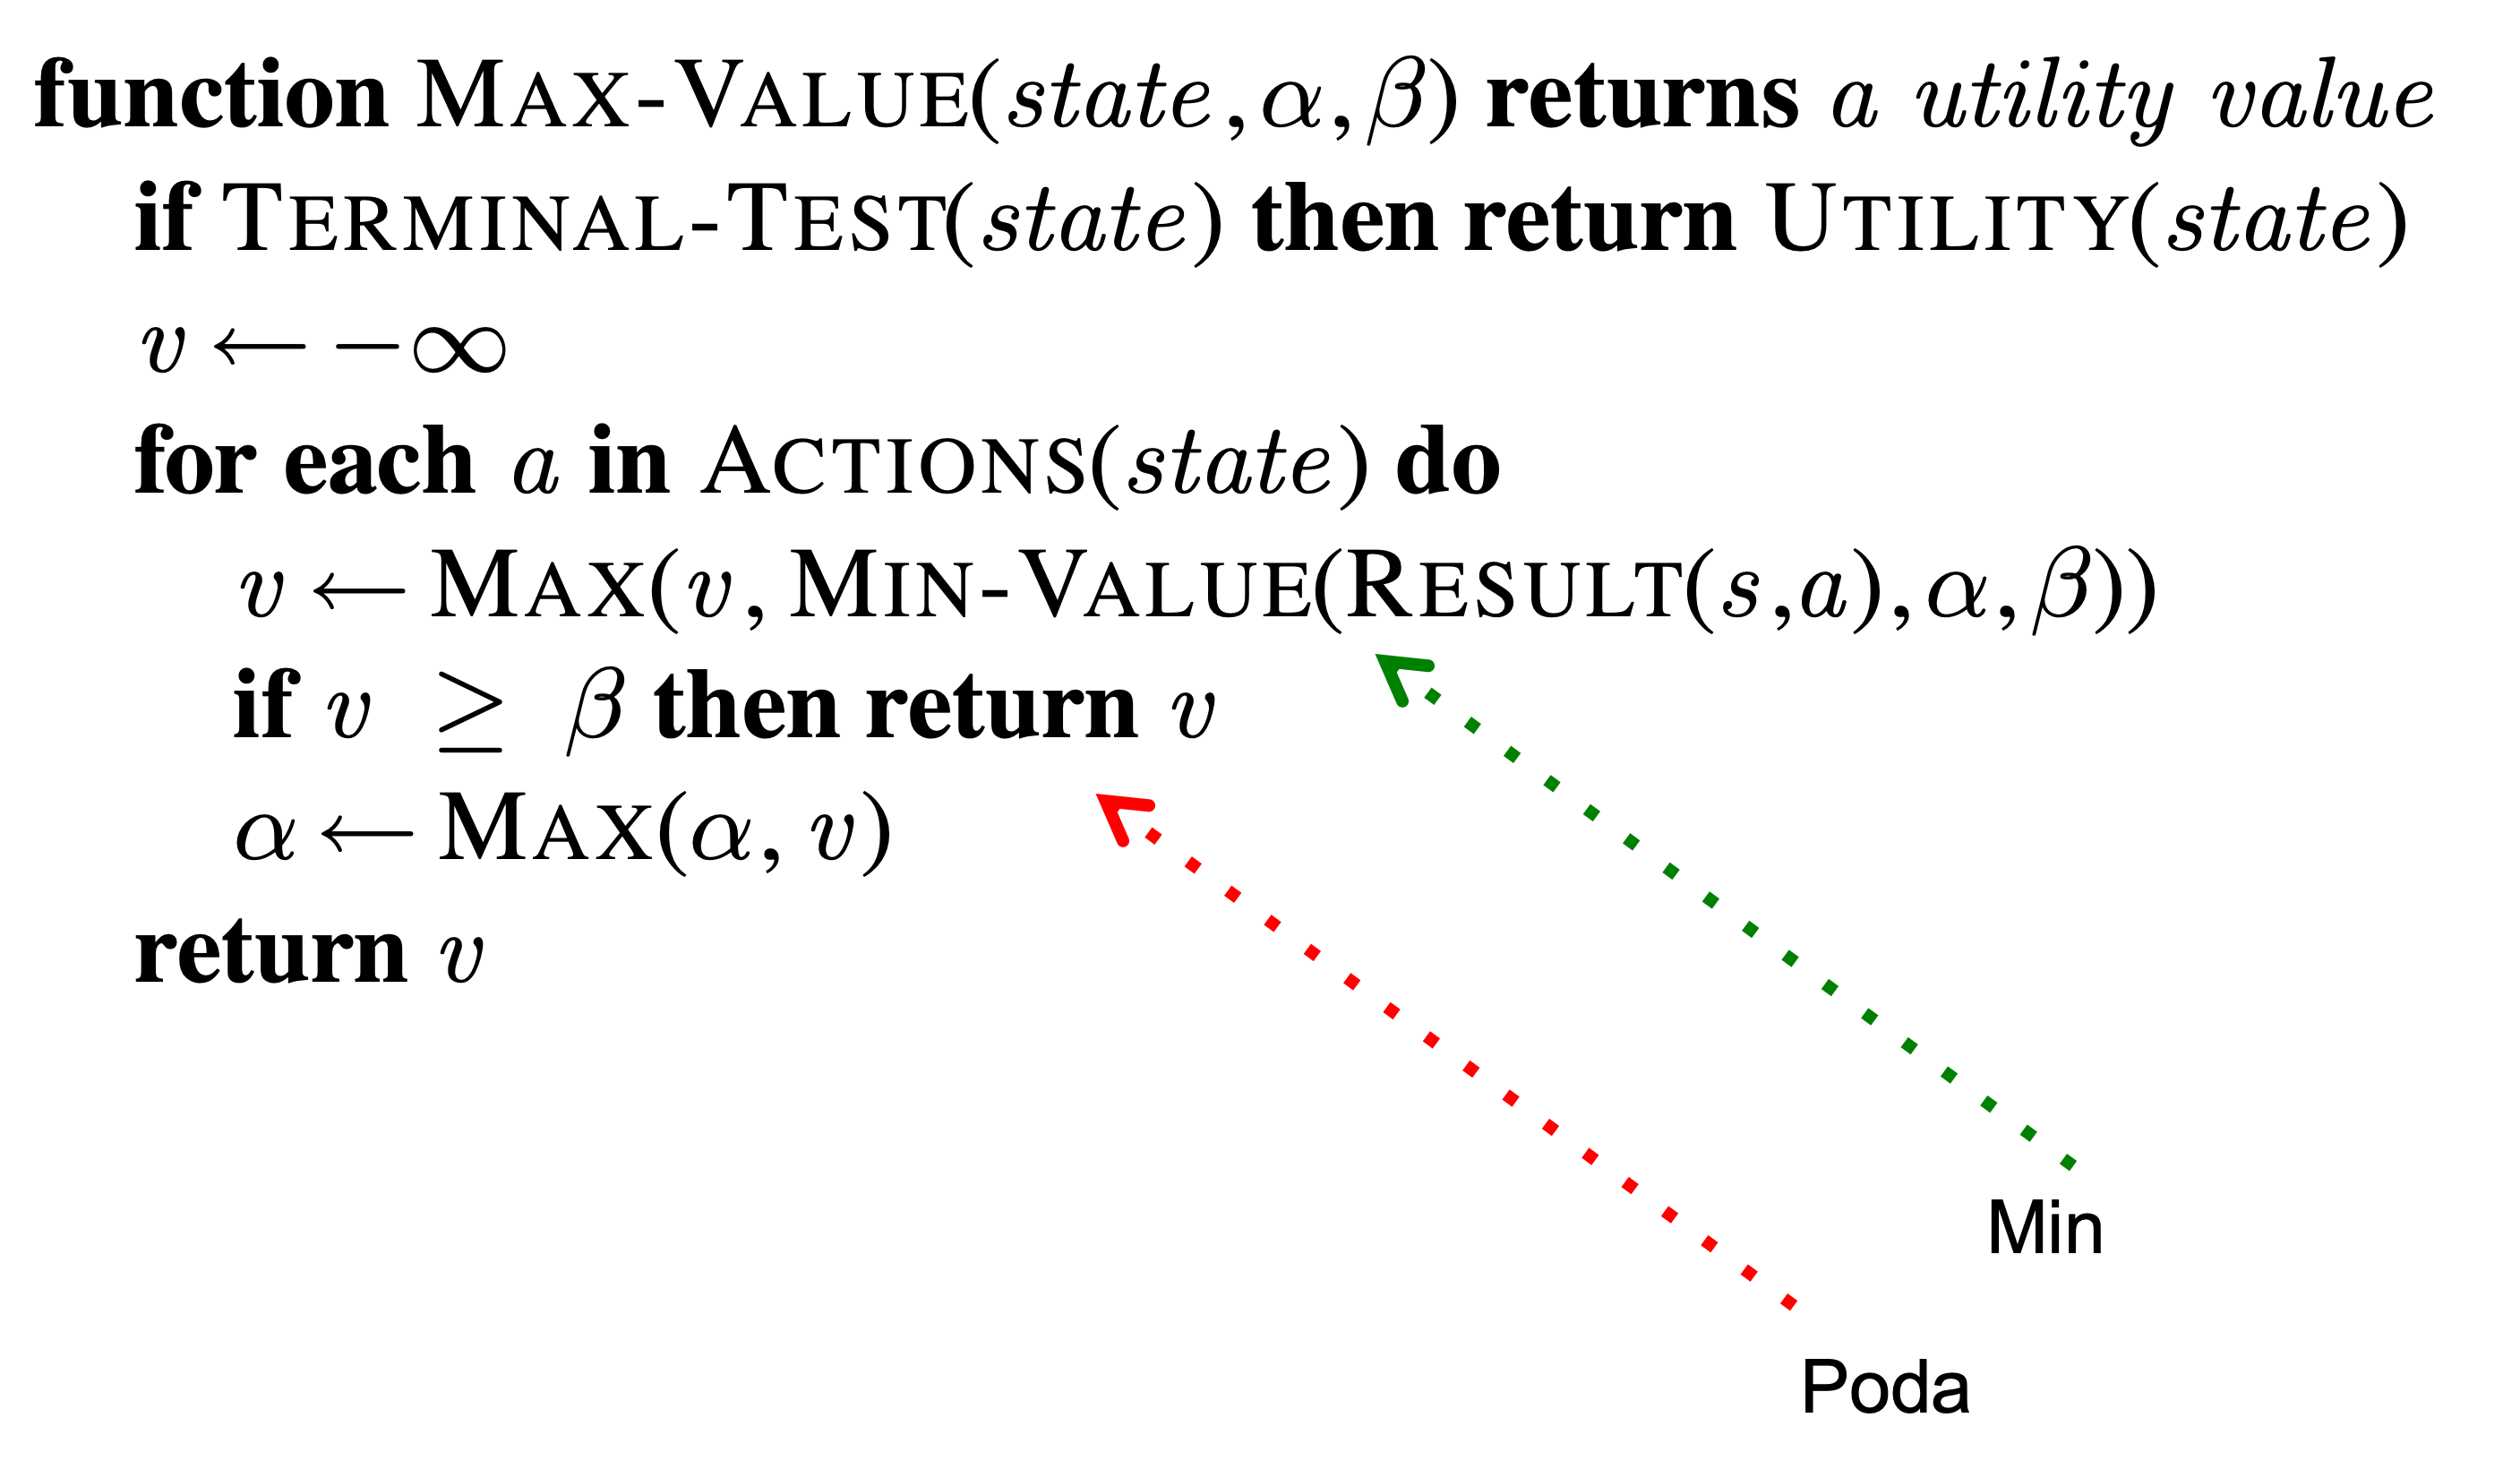
\includegraphics[scale=0.45]{./img/alfabeta2}
\end{figure}
\end{frame} 

%%%%%%%%%%%%%%%%%%%%%%%%%%%%%%%%

\begin{frame} \frametitle{Poda $\alpha$-$\beta$ } \small

\begin{figure}
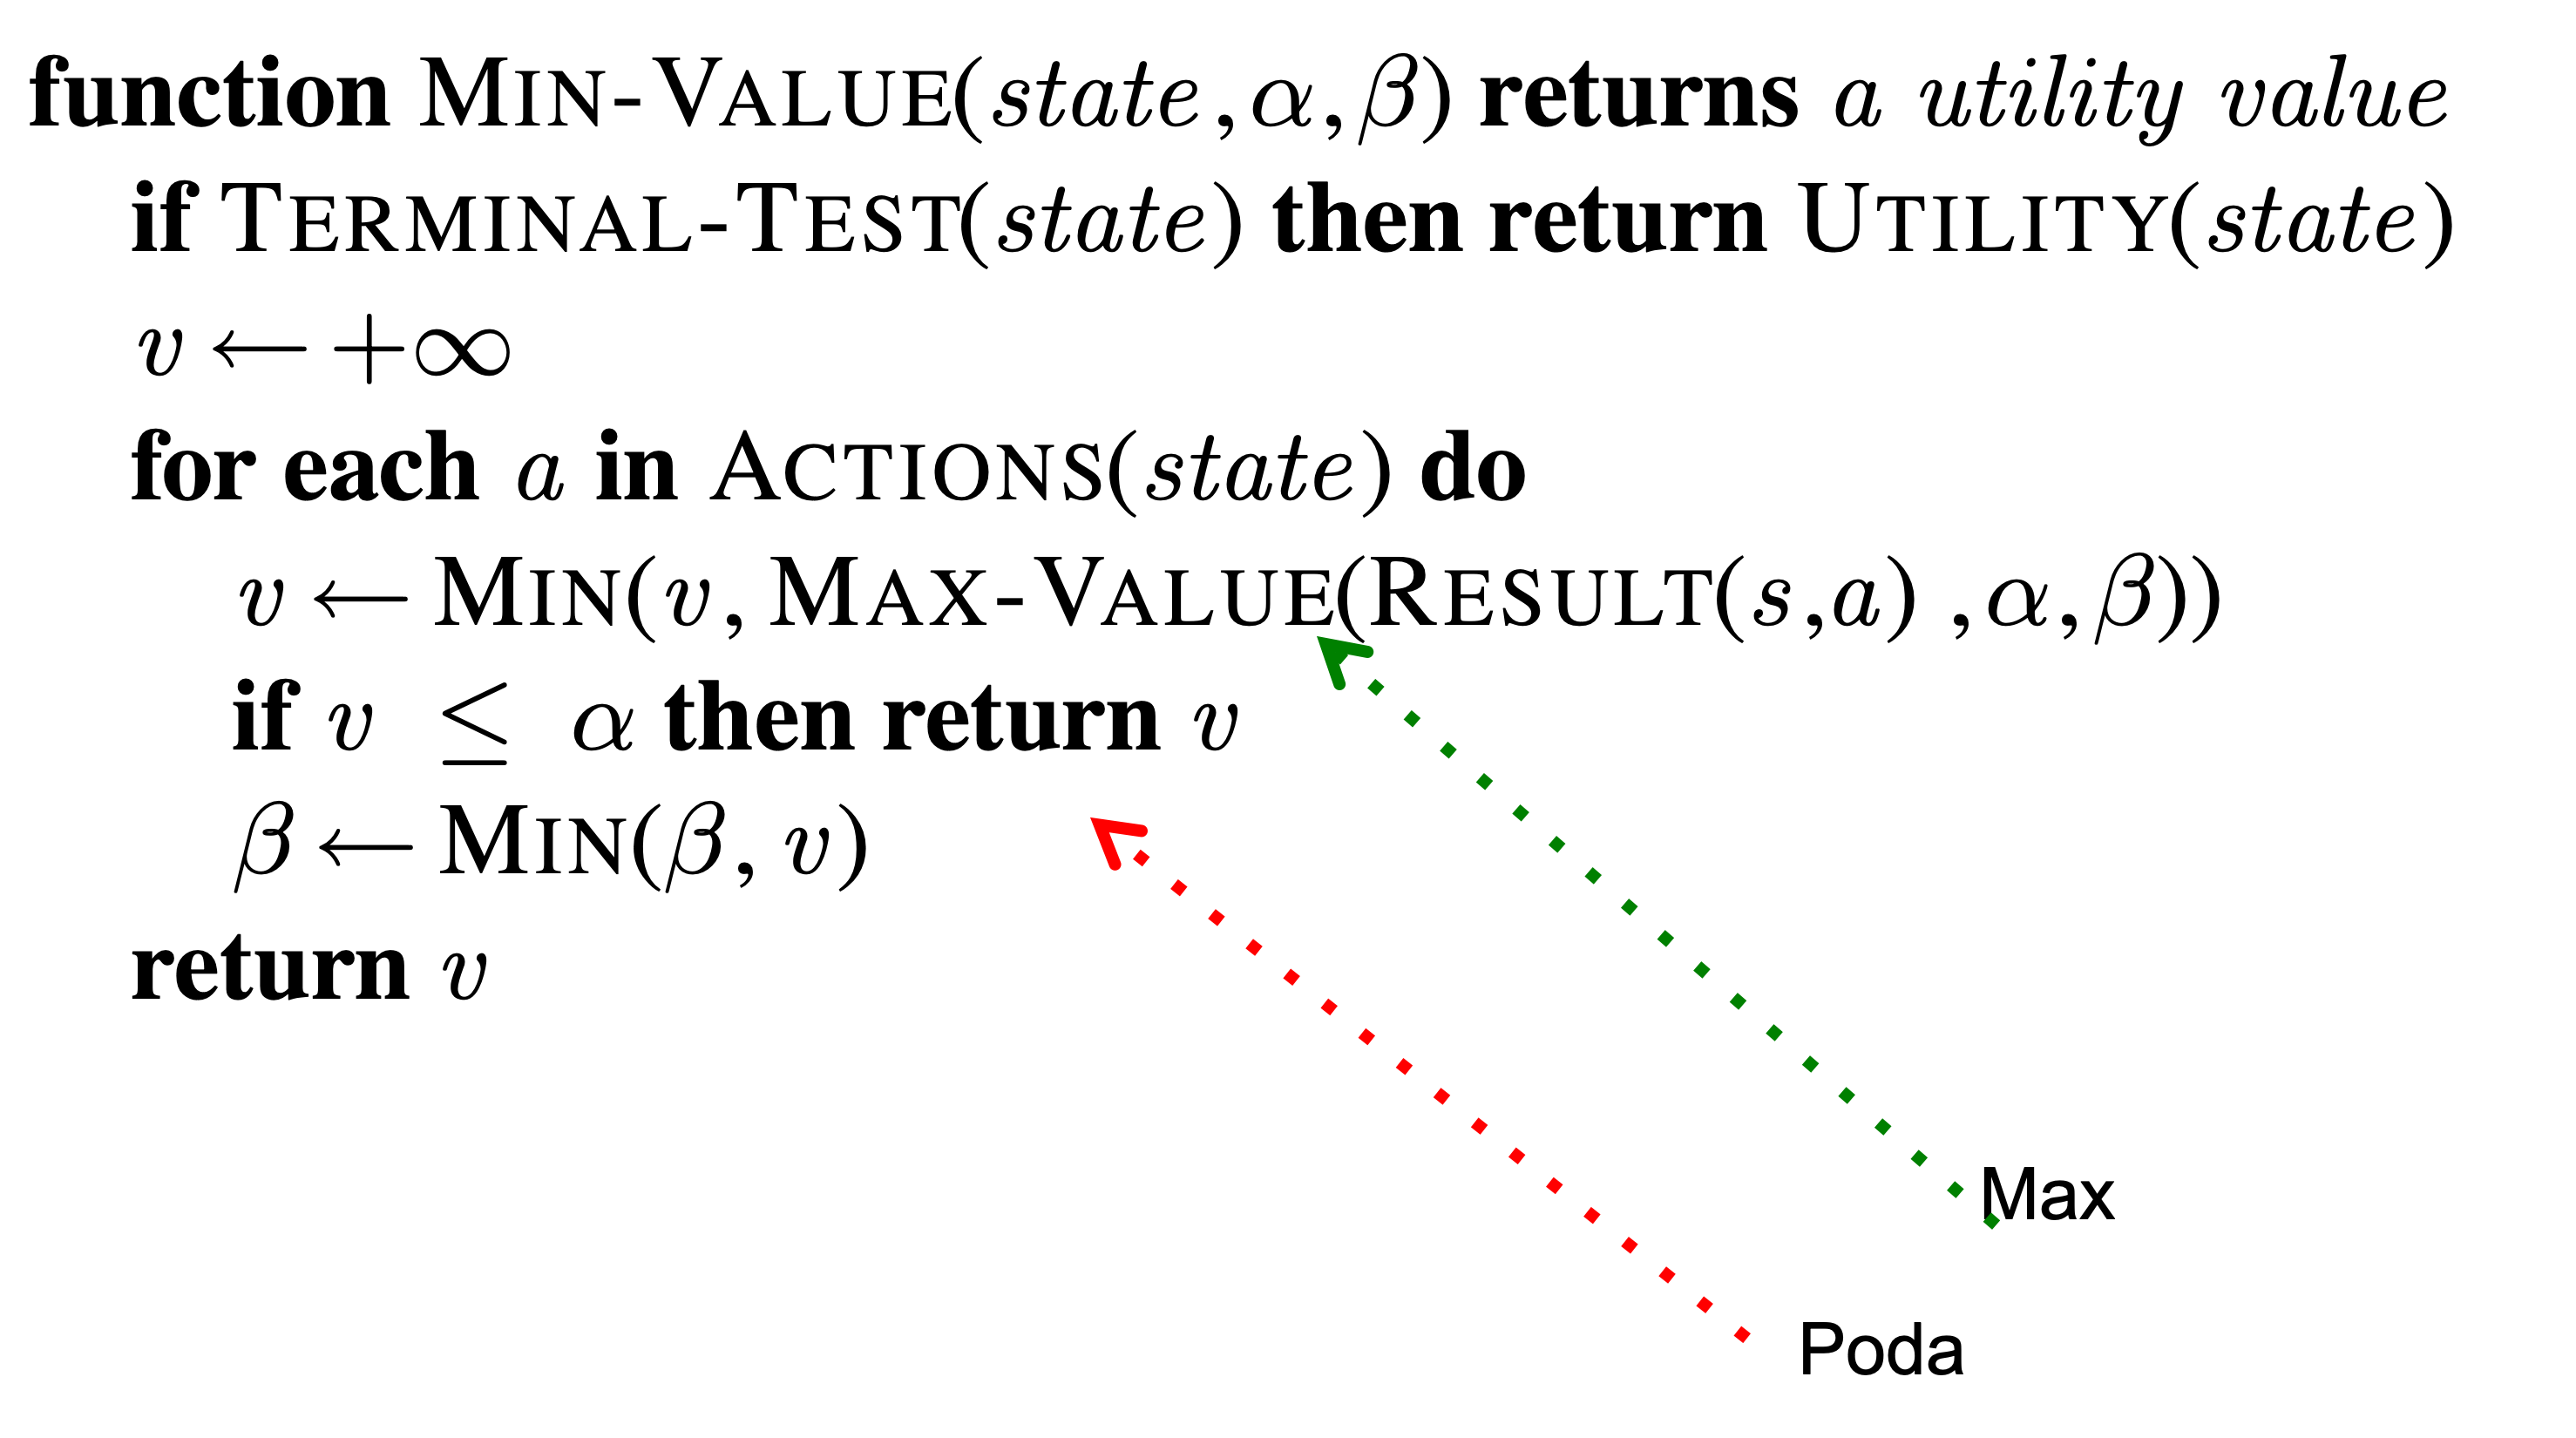
\includegraphics[scale=0.45]{./img/alfabeta3}
\end{figure}
\end{frame} 

%%%%%%%%%%%%%%%%%%%%%%%%%%%%%%%%

\begin{frame} \frametitle{Poda $\alpha$-$\beta$ Ed. 4 } \small

\begin{figure}
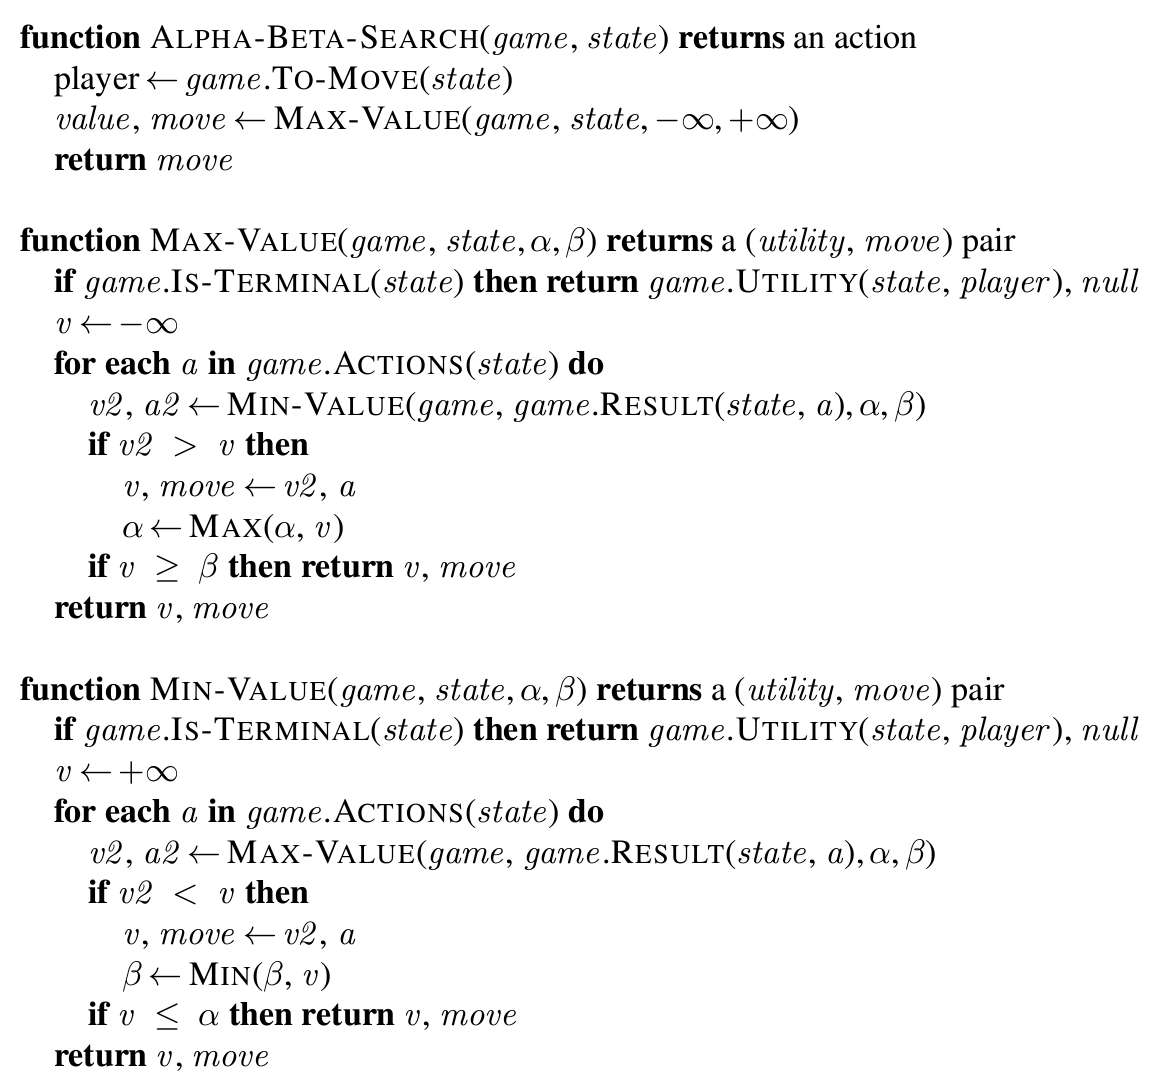
\includegraphics[scale=0.3]{./img/AlfaBetaNew}
\end{figure}
\end{frame} 

%%%%%%%%%%%%%%%%%%%%%%%%%%%%%%%%

\begin{frame} \frametitle{Ejemplo Poda $\alpha$-$\beta$ } \small

\begin{figure}
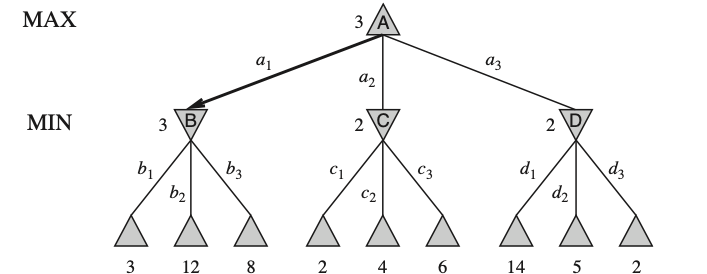
\includegraphics[scale=0.45]{./img/ejemploAlfabeta}
\end{figure}
\end{frame} 




%%%%%%%%%%%%%%%%%%%%%%%%%%%%%%%%

\begin{frame} \frametitle{Ejemplo Poda $\alpha$-$\beta$ } \small

\begin{figure}
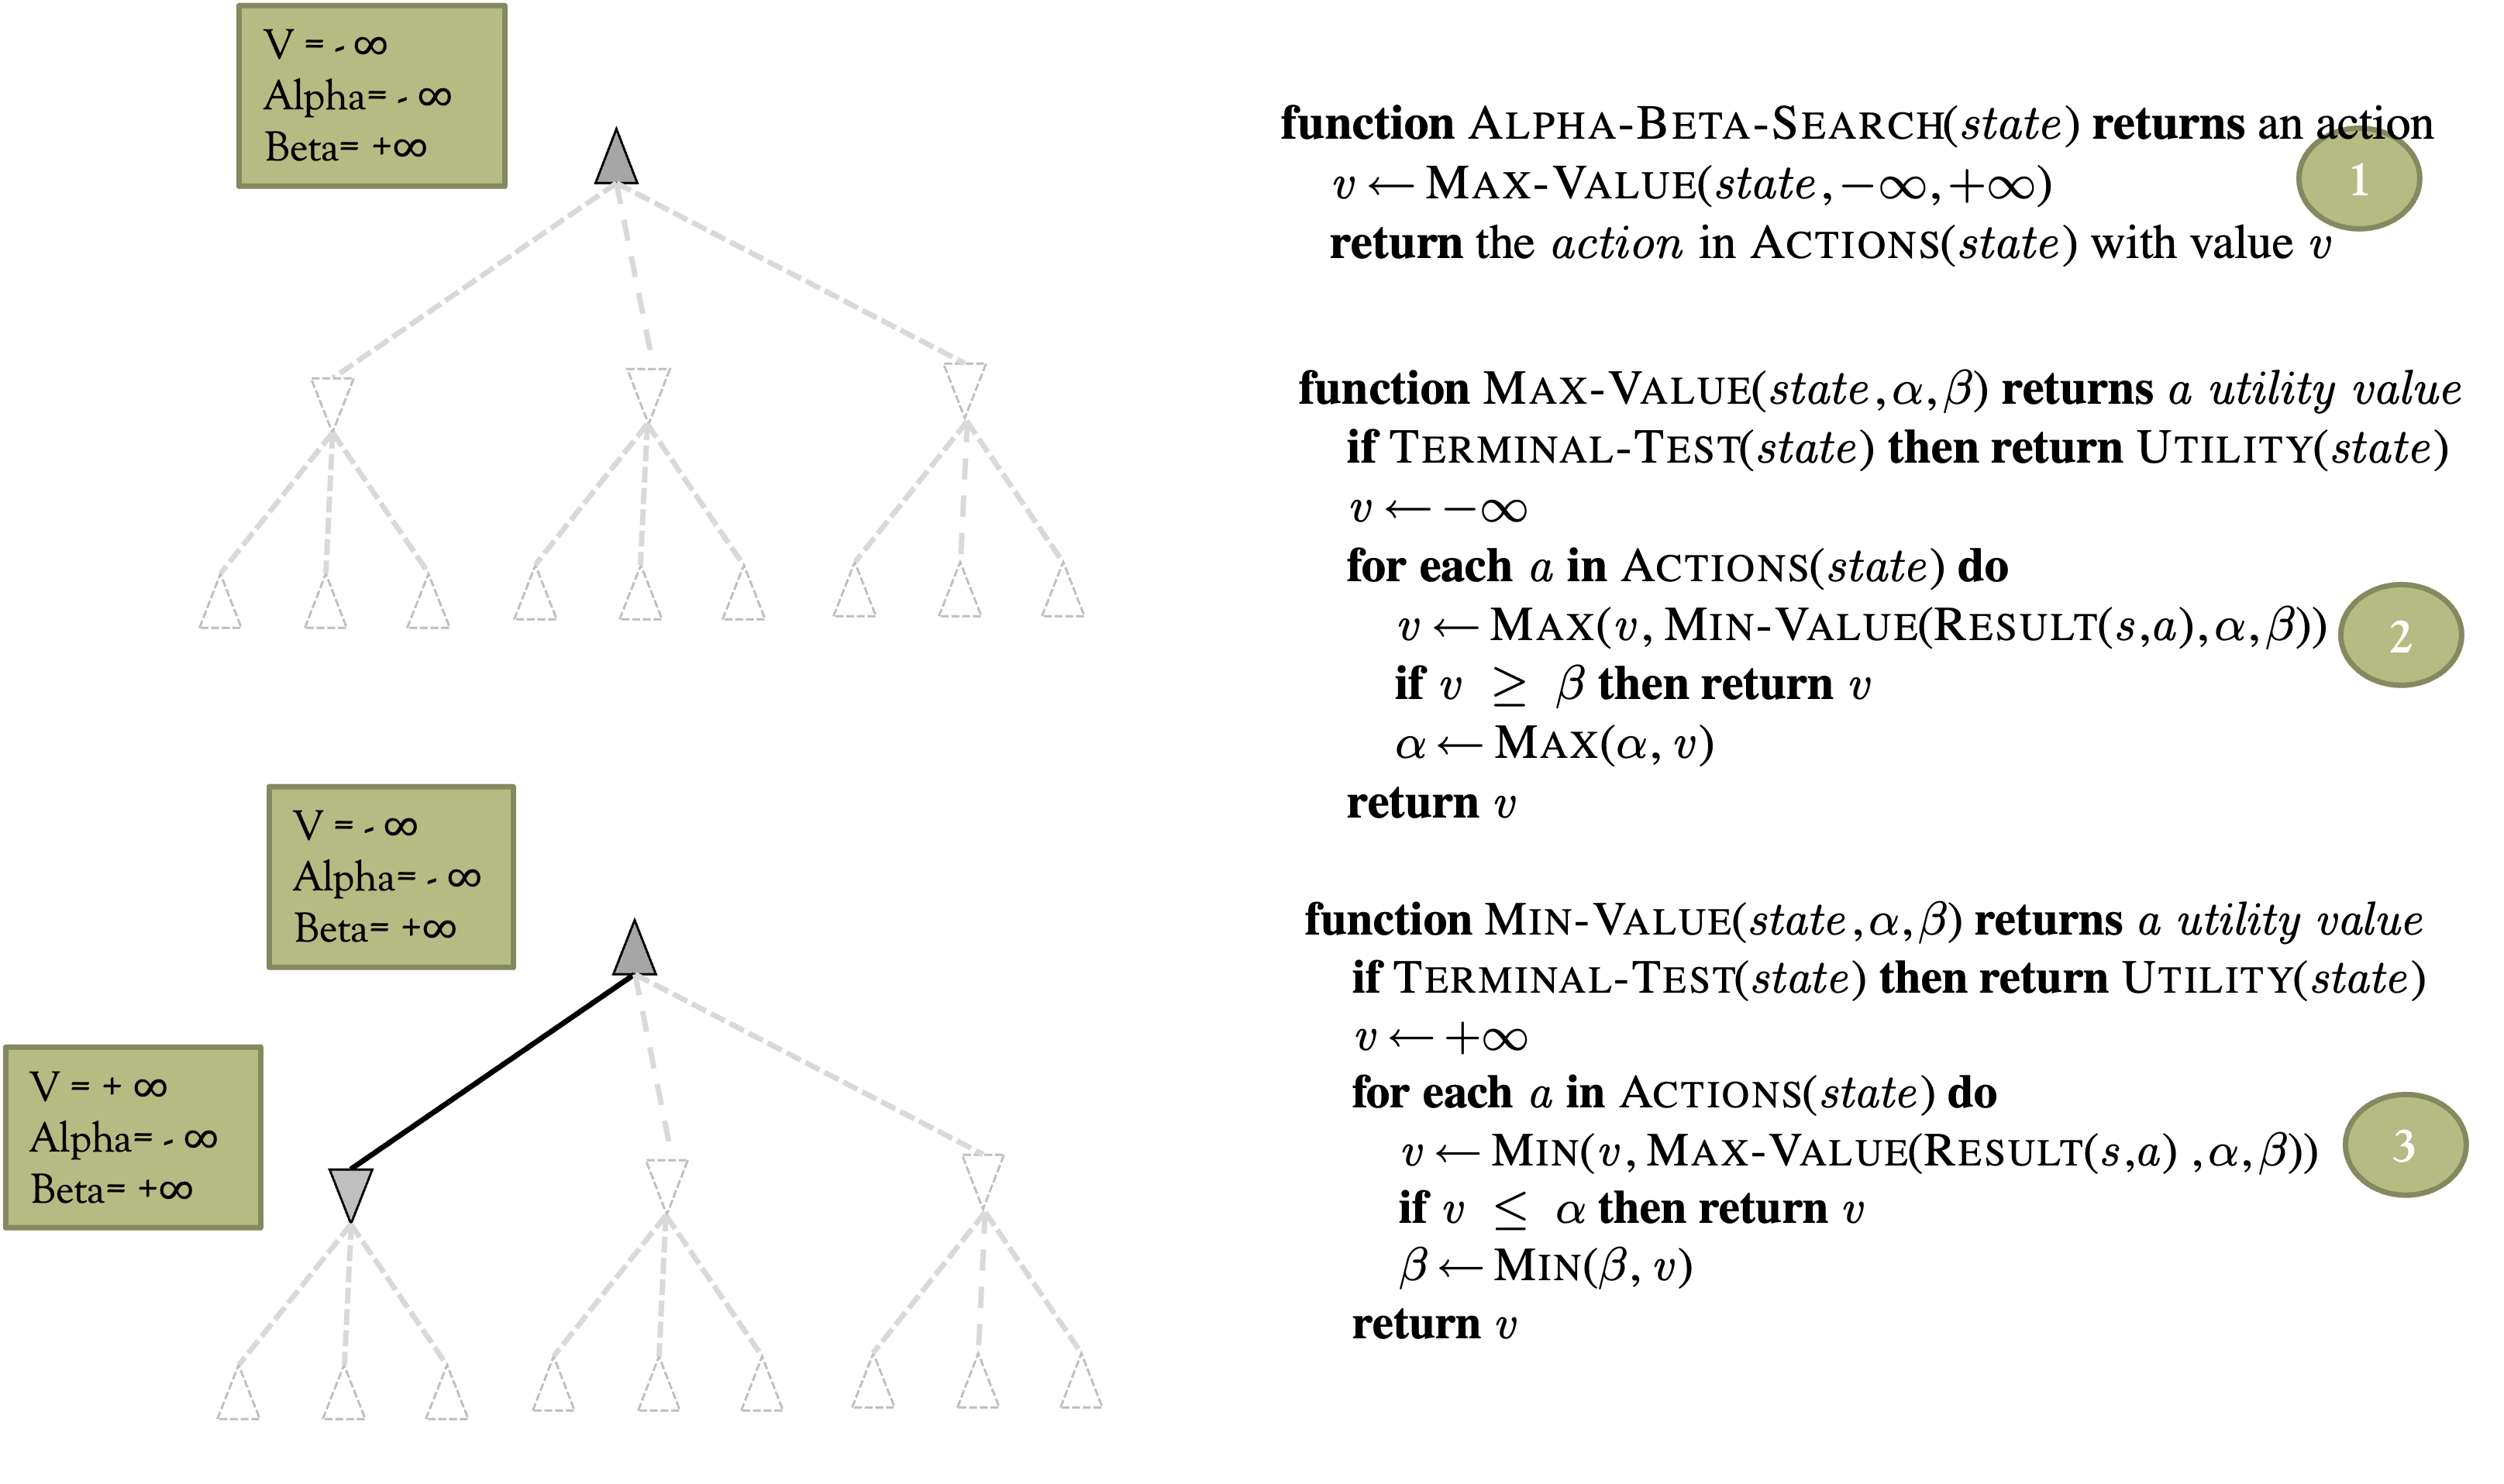
\includegraphics[scale=0.4]{./img/ejemploAlfabeta1}
\end{figure}
\end{frame} 

%%%%%%%%%%%%%%%%%%%%%%%%%%%%%%%%

\begin{frame} \frametitle{Ejemplo Poda $\alpha$-$\beta$ } \small

\begin{figure}
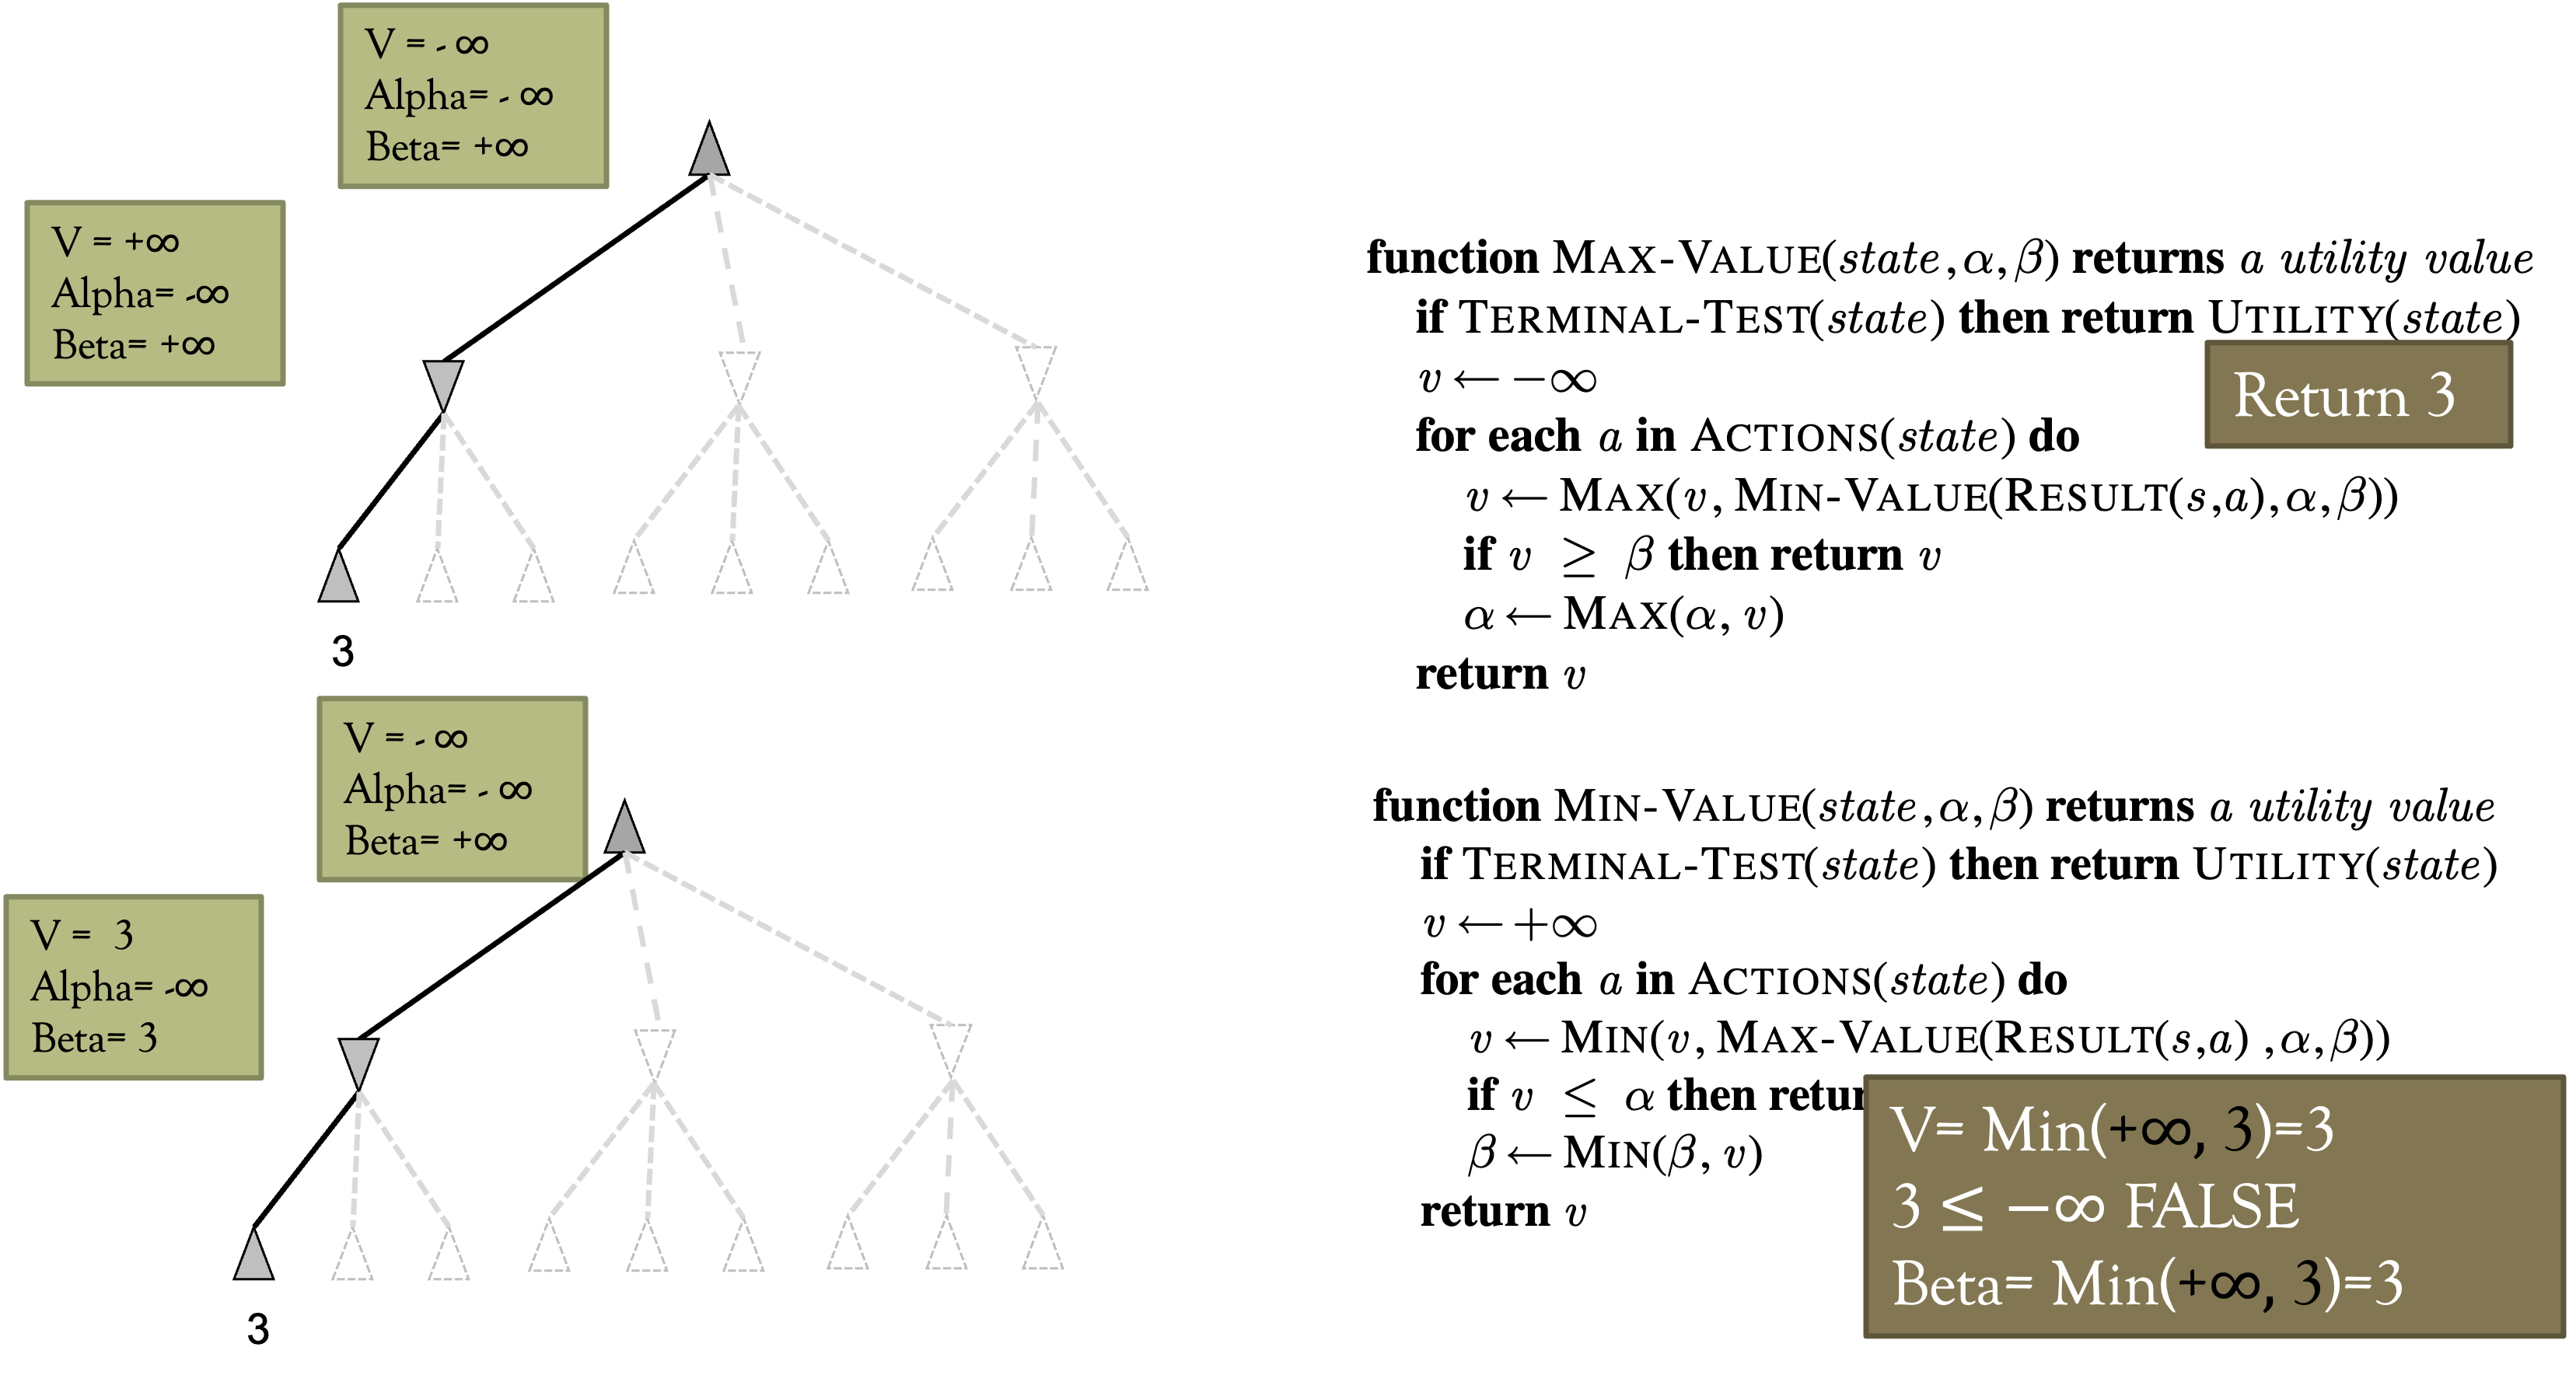
\includegraphics[scale=0.45]{./img/ejemploAlfabeta2}
\end{figure}
\end{frame} 

%%%%%%%%%%%%%%%%%%%%%%%%%%%%%%%%

\begin{frame} \frametitle{Ejemplo Poda $\alpha$-$\beta$ } \small

\begin{figure}
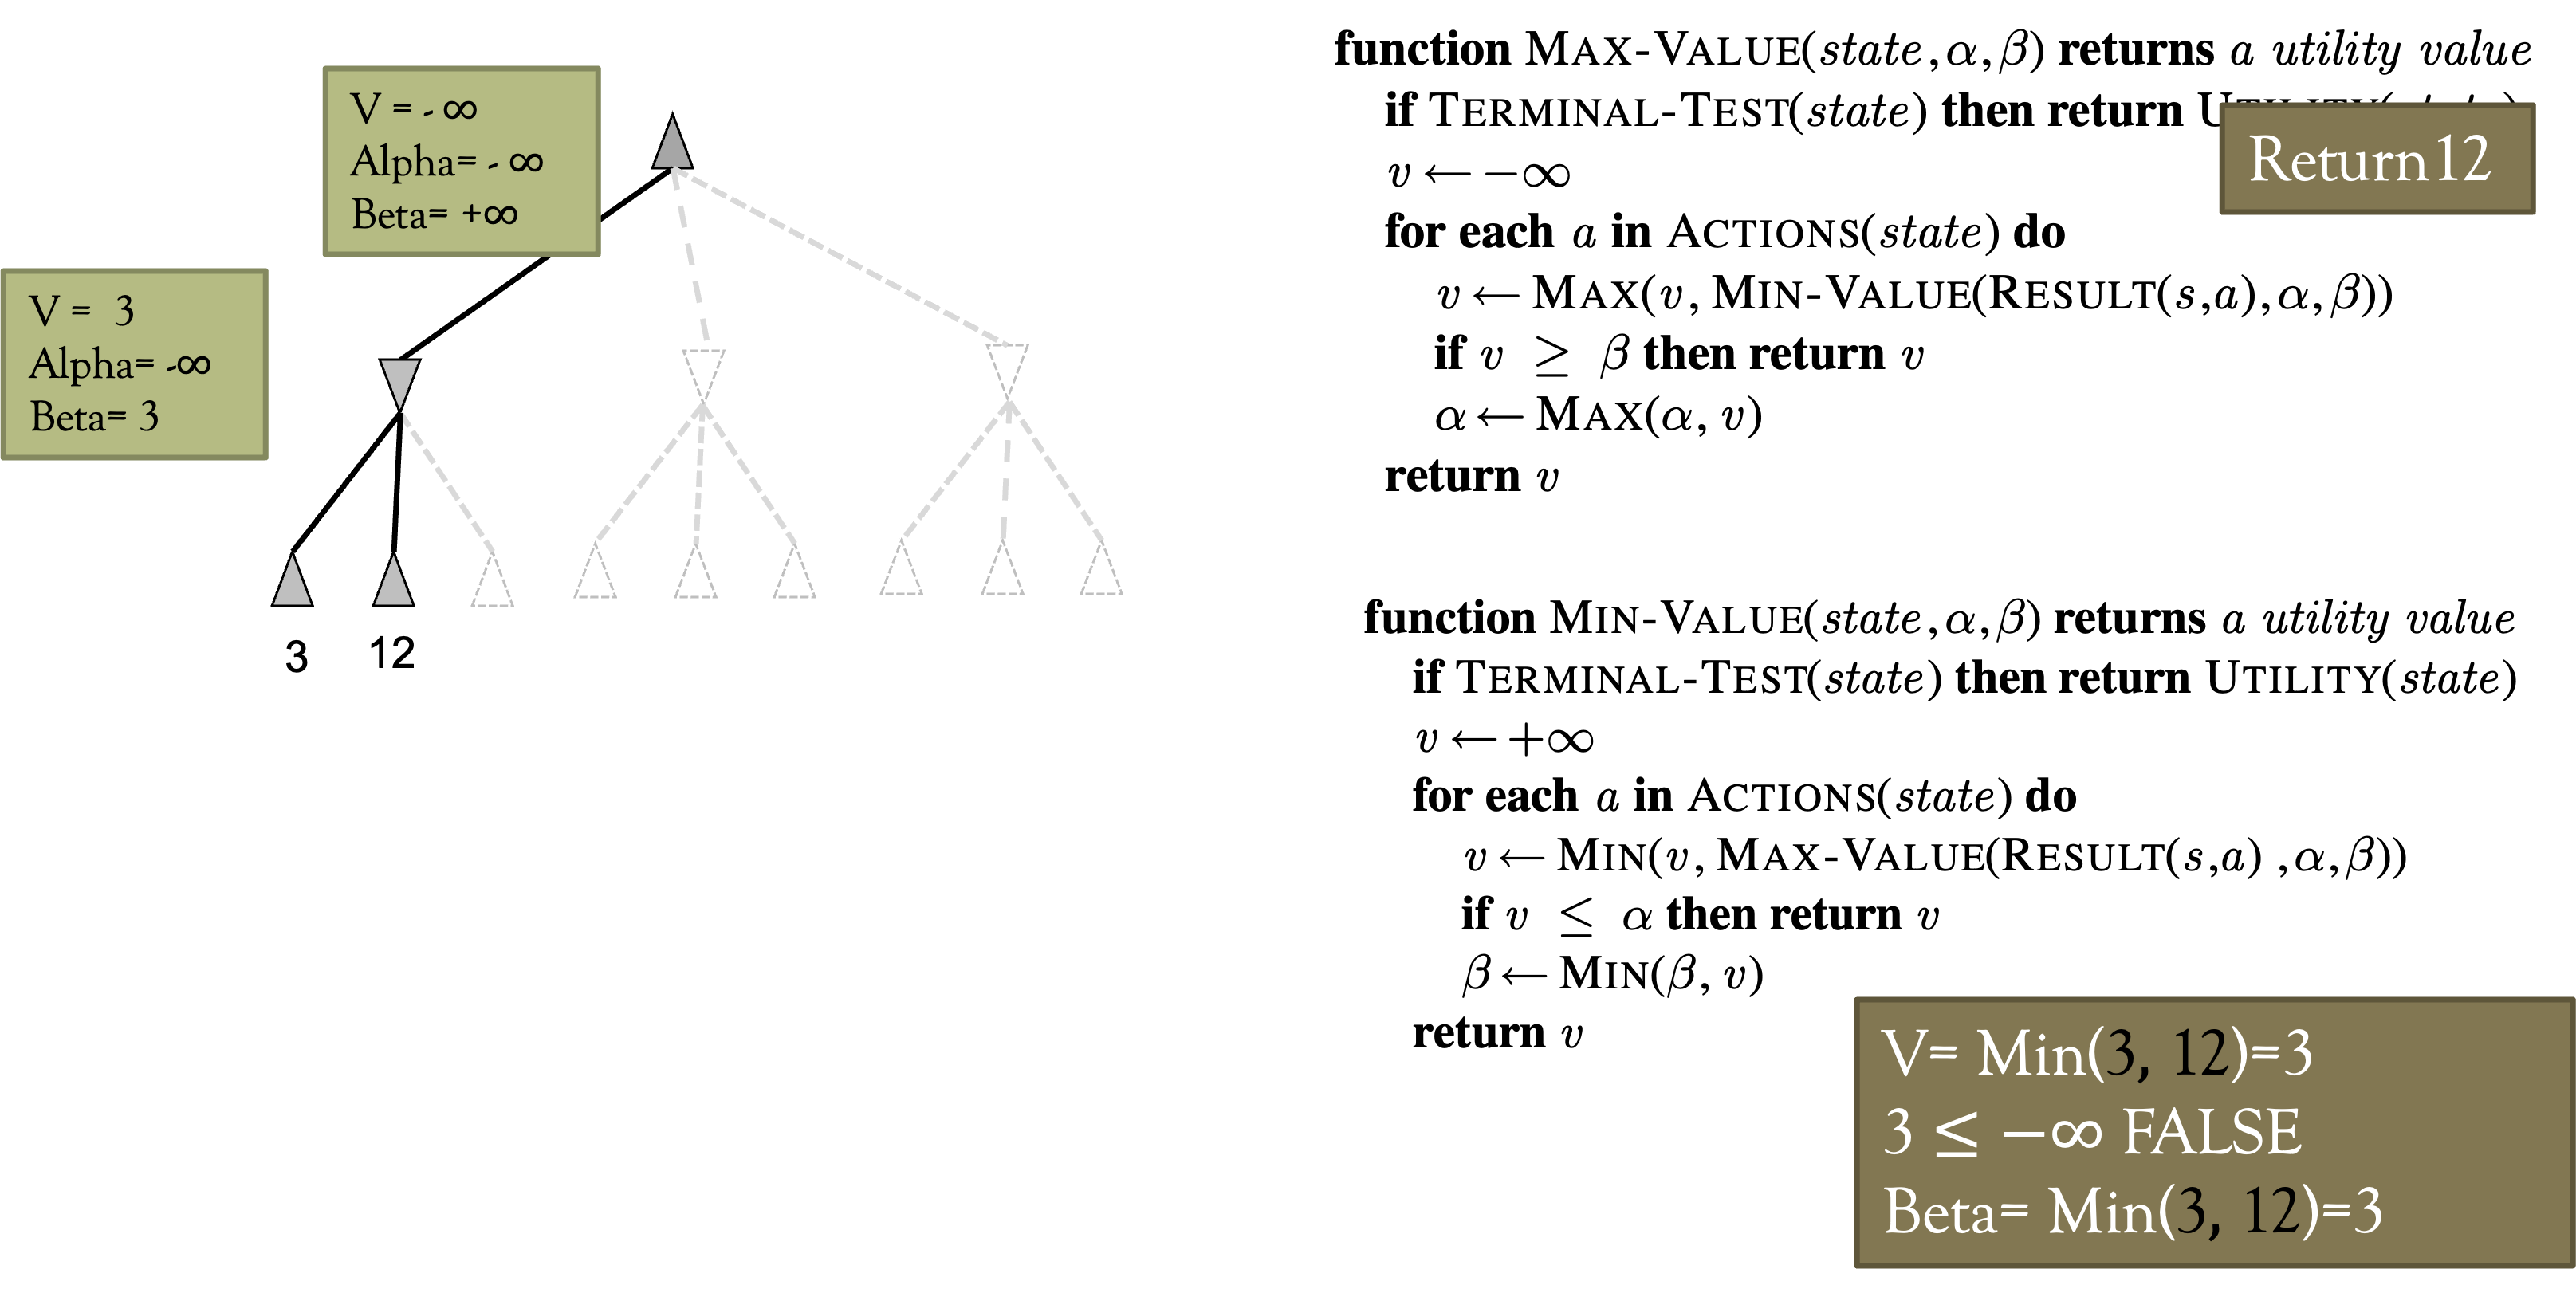
\includegraphics[scale=0.45]{./img/ejemploAlfabeta3}
\end{figure}
\end{frame} 

%%%%%%%%%%%%%%%%%%%%%%%%%%%%%%%%

\begin{frame} \frametitle{Ejemplo Poda $\alpha$-$\beta$ } \small

\begin{figure}
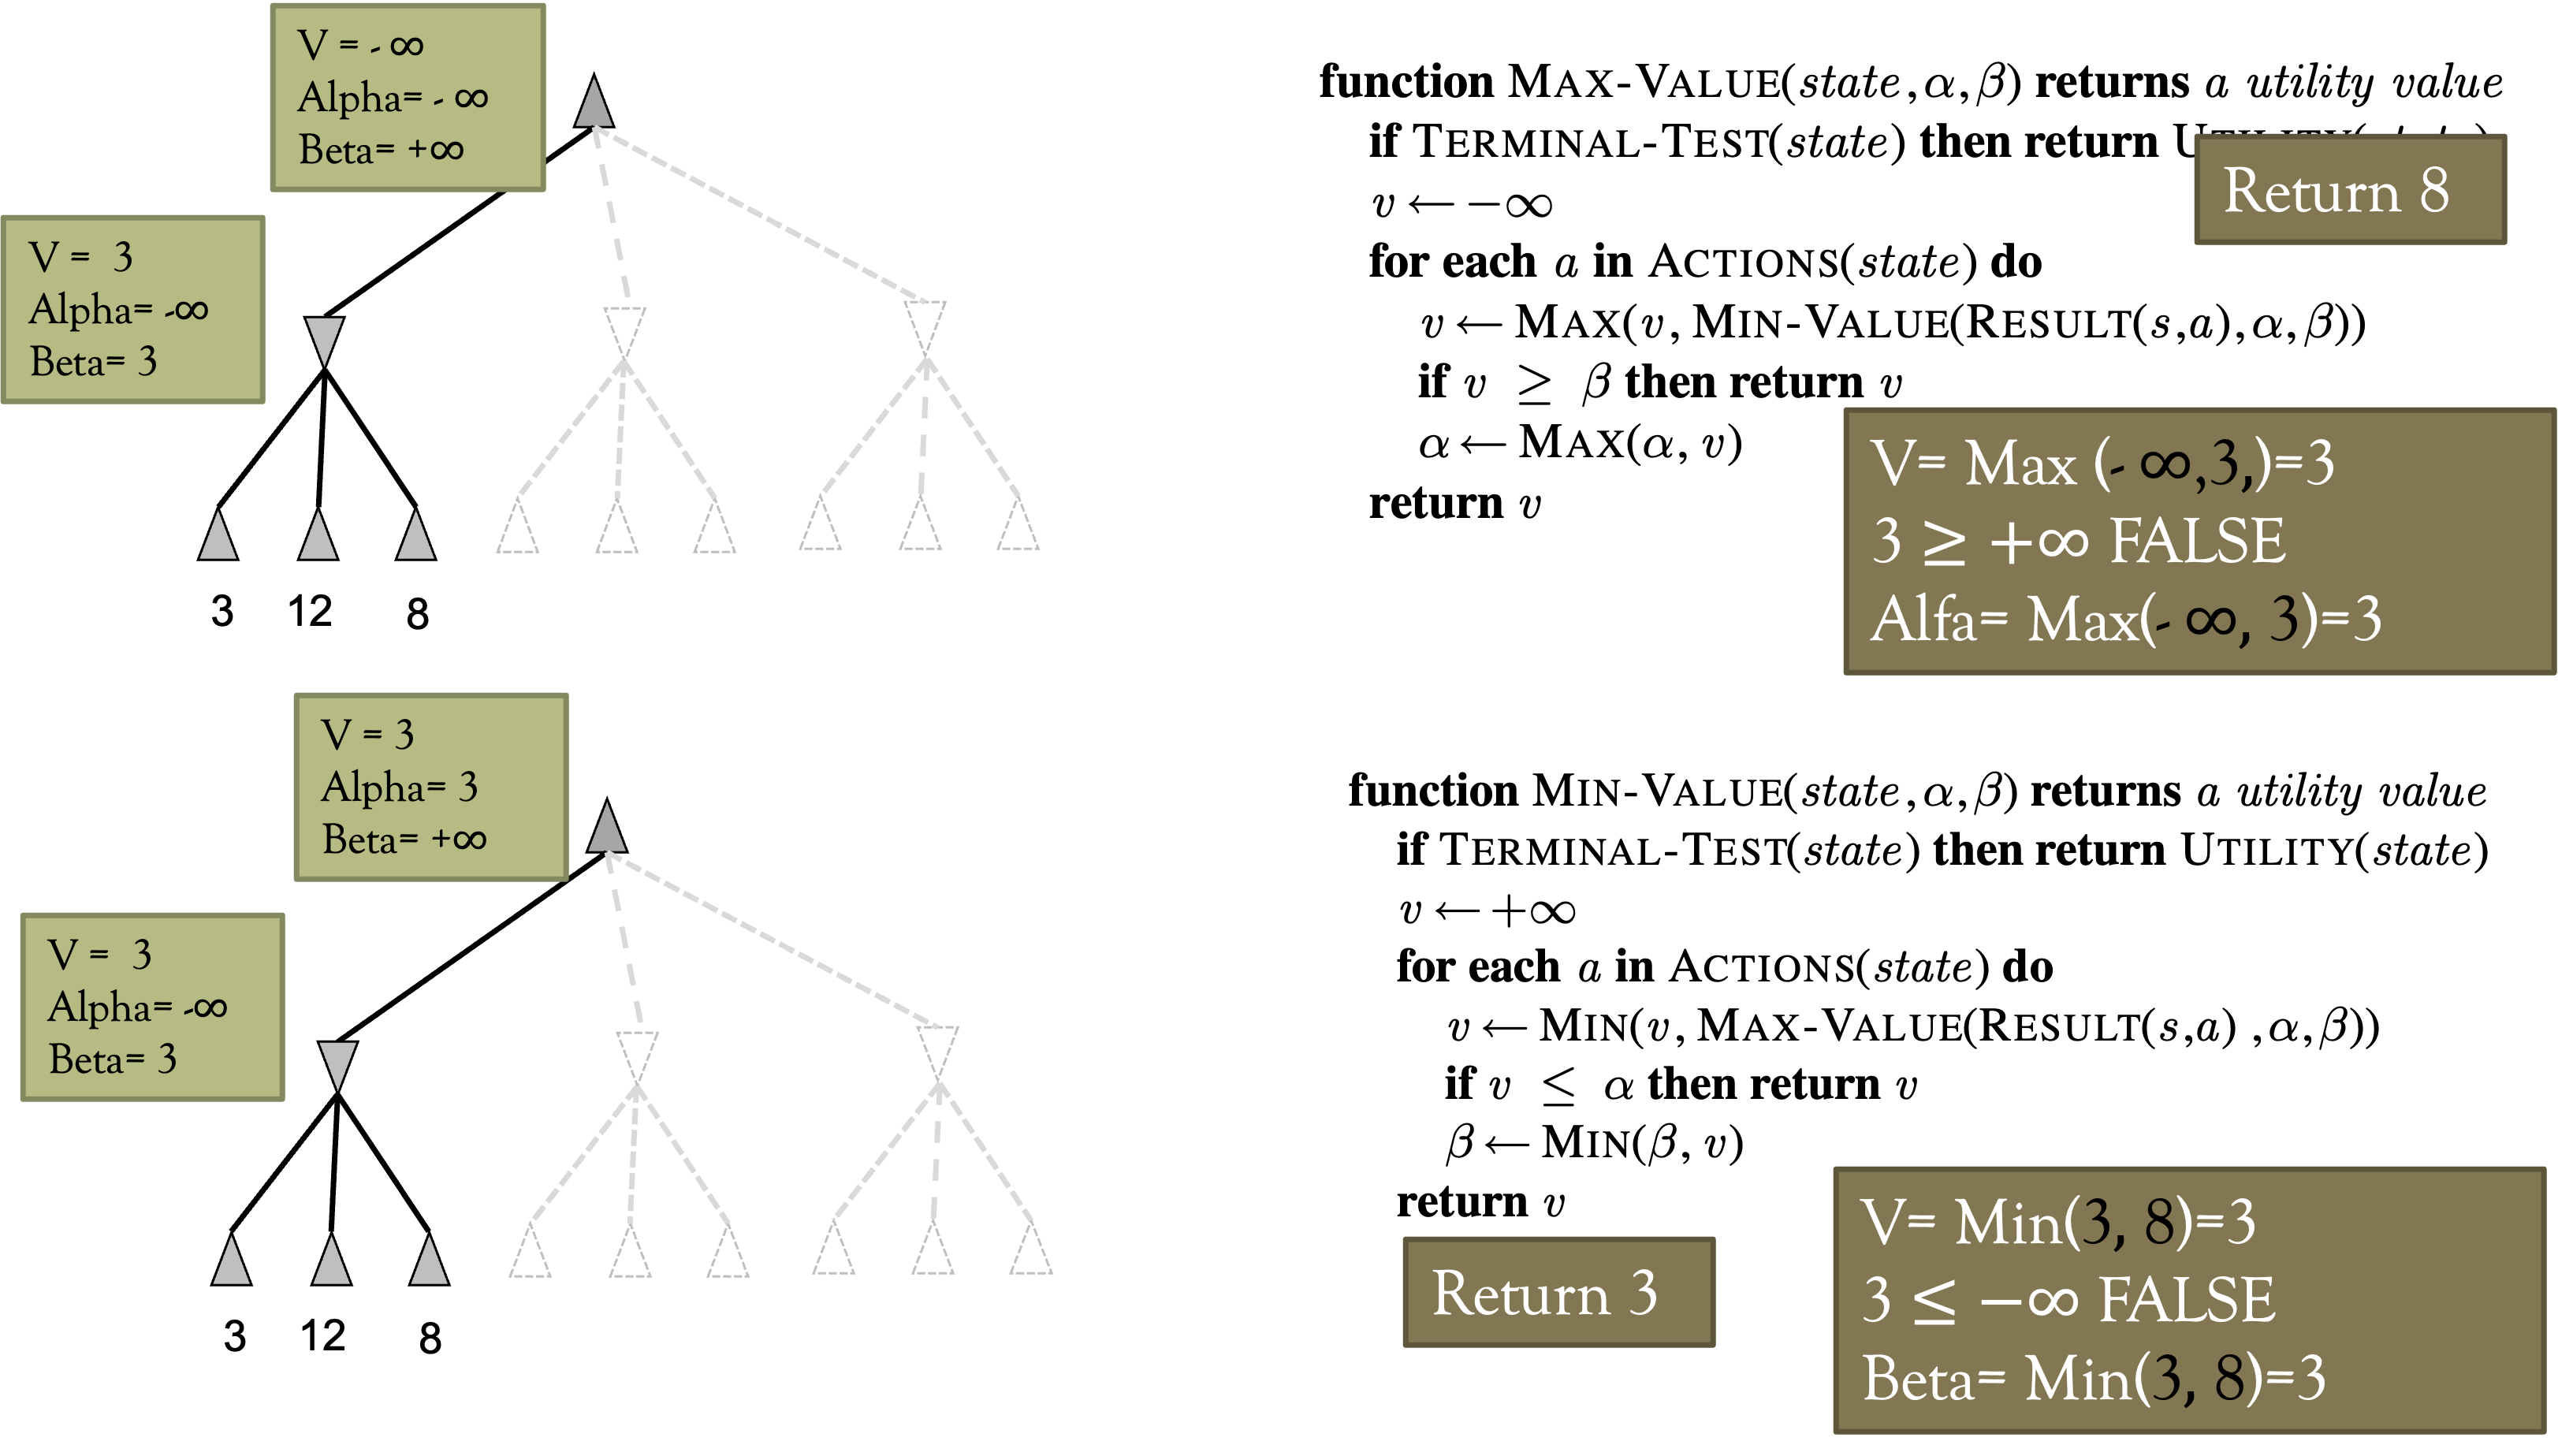
\includegraphics[scale=0.4]{./img/ejemploAlfabeta4}
\end{figure}
\end{frame} 

%%%%%%%%%%%%%%%%%%%%%%%%%%%%%%%%

\begin{frame} \frametitle{Ejemplo Poda $\alpha$-$\beta$ } \small

\begin{figure}
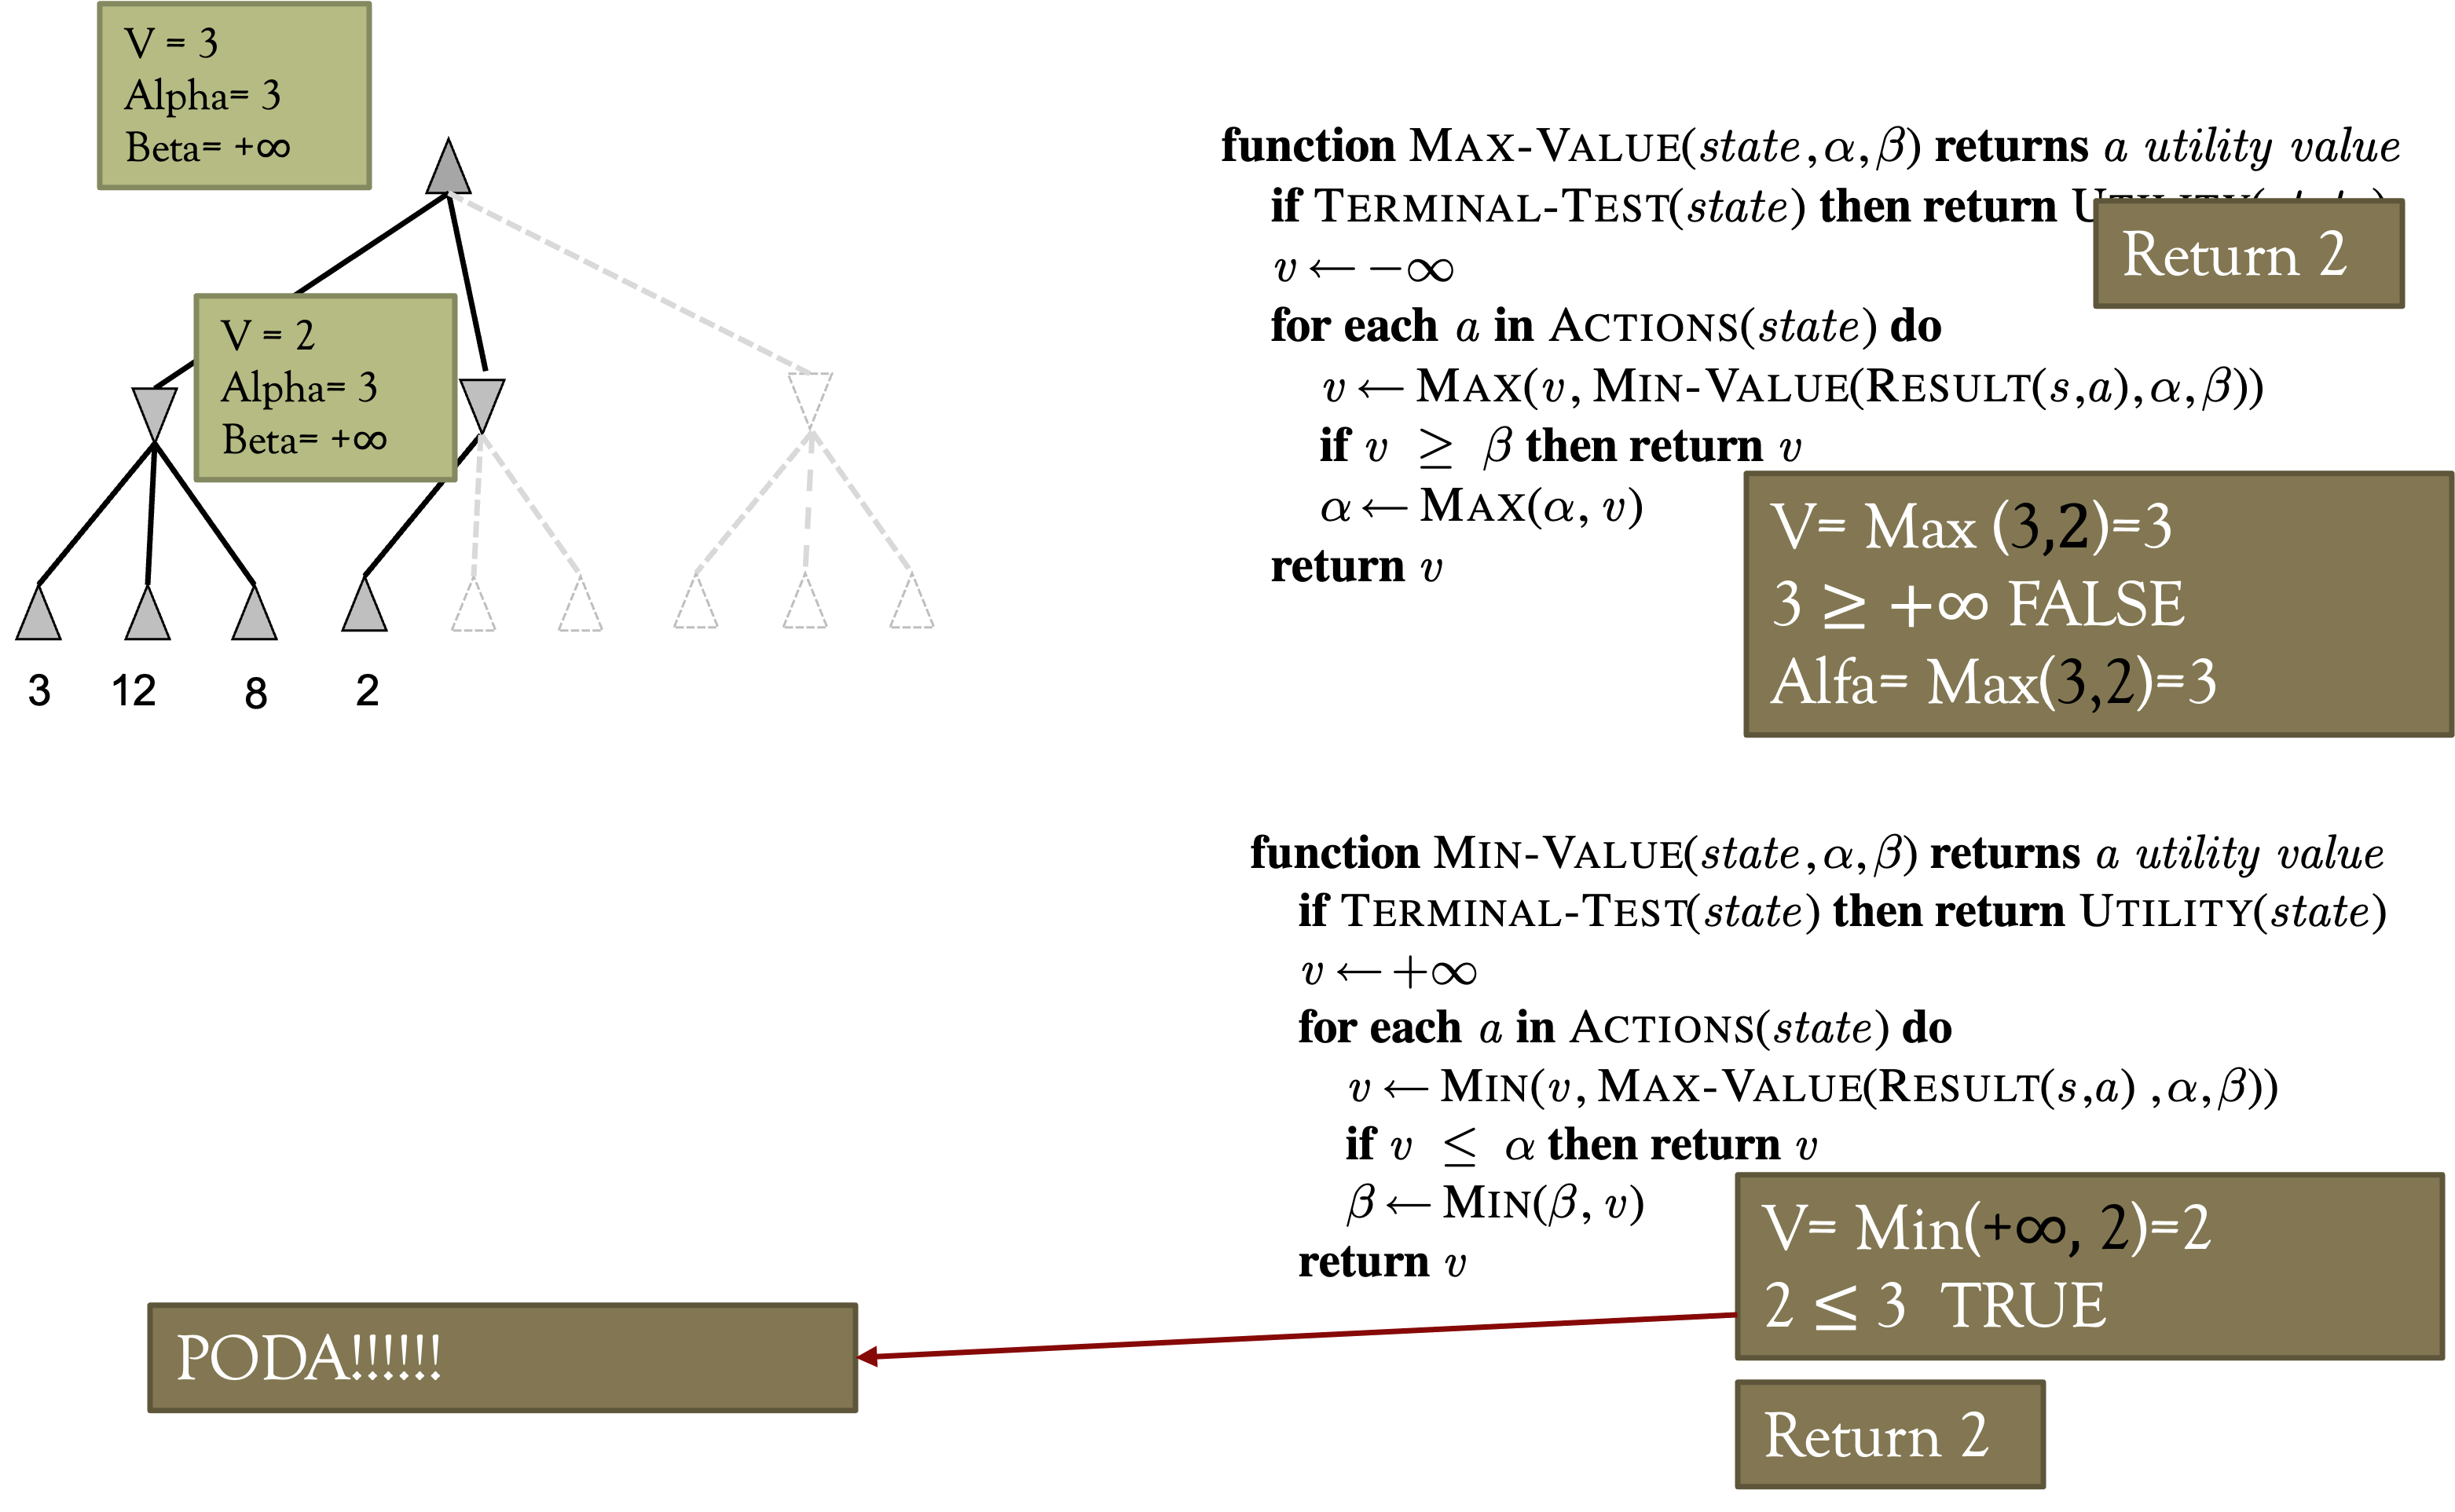
\includegraphics[scale=0.4]{./img/ejemploAlfabeta5}
\end{figure}
\end{frame} 

%%%%%%%%%%%%%%%%%%%%%%%%%%%%%%%%

\begin{frame} \frametitle{Ejemplo Poda $\alpha$-$\beta$ } \small

\begin{figure}
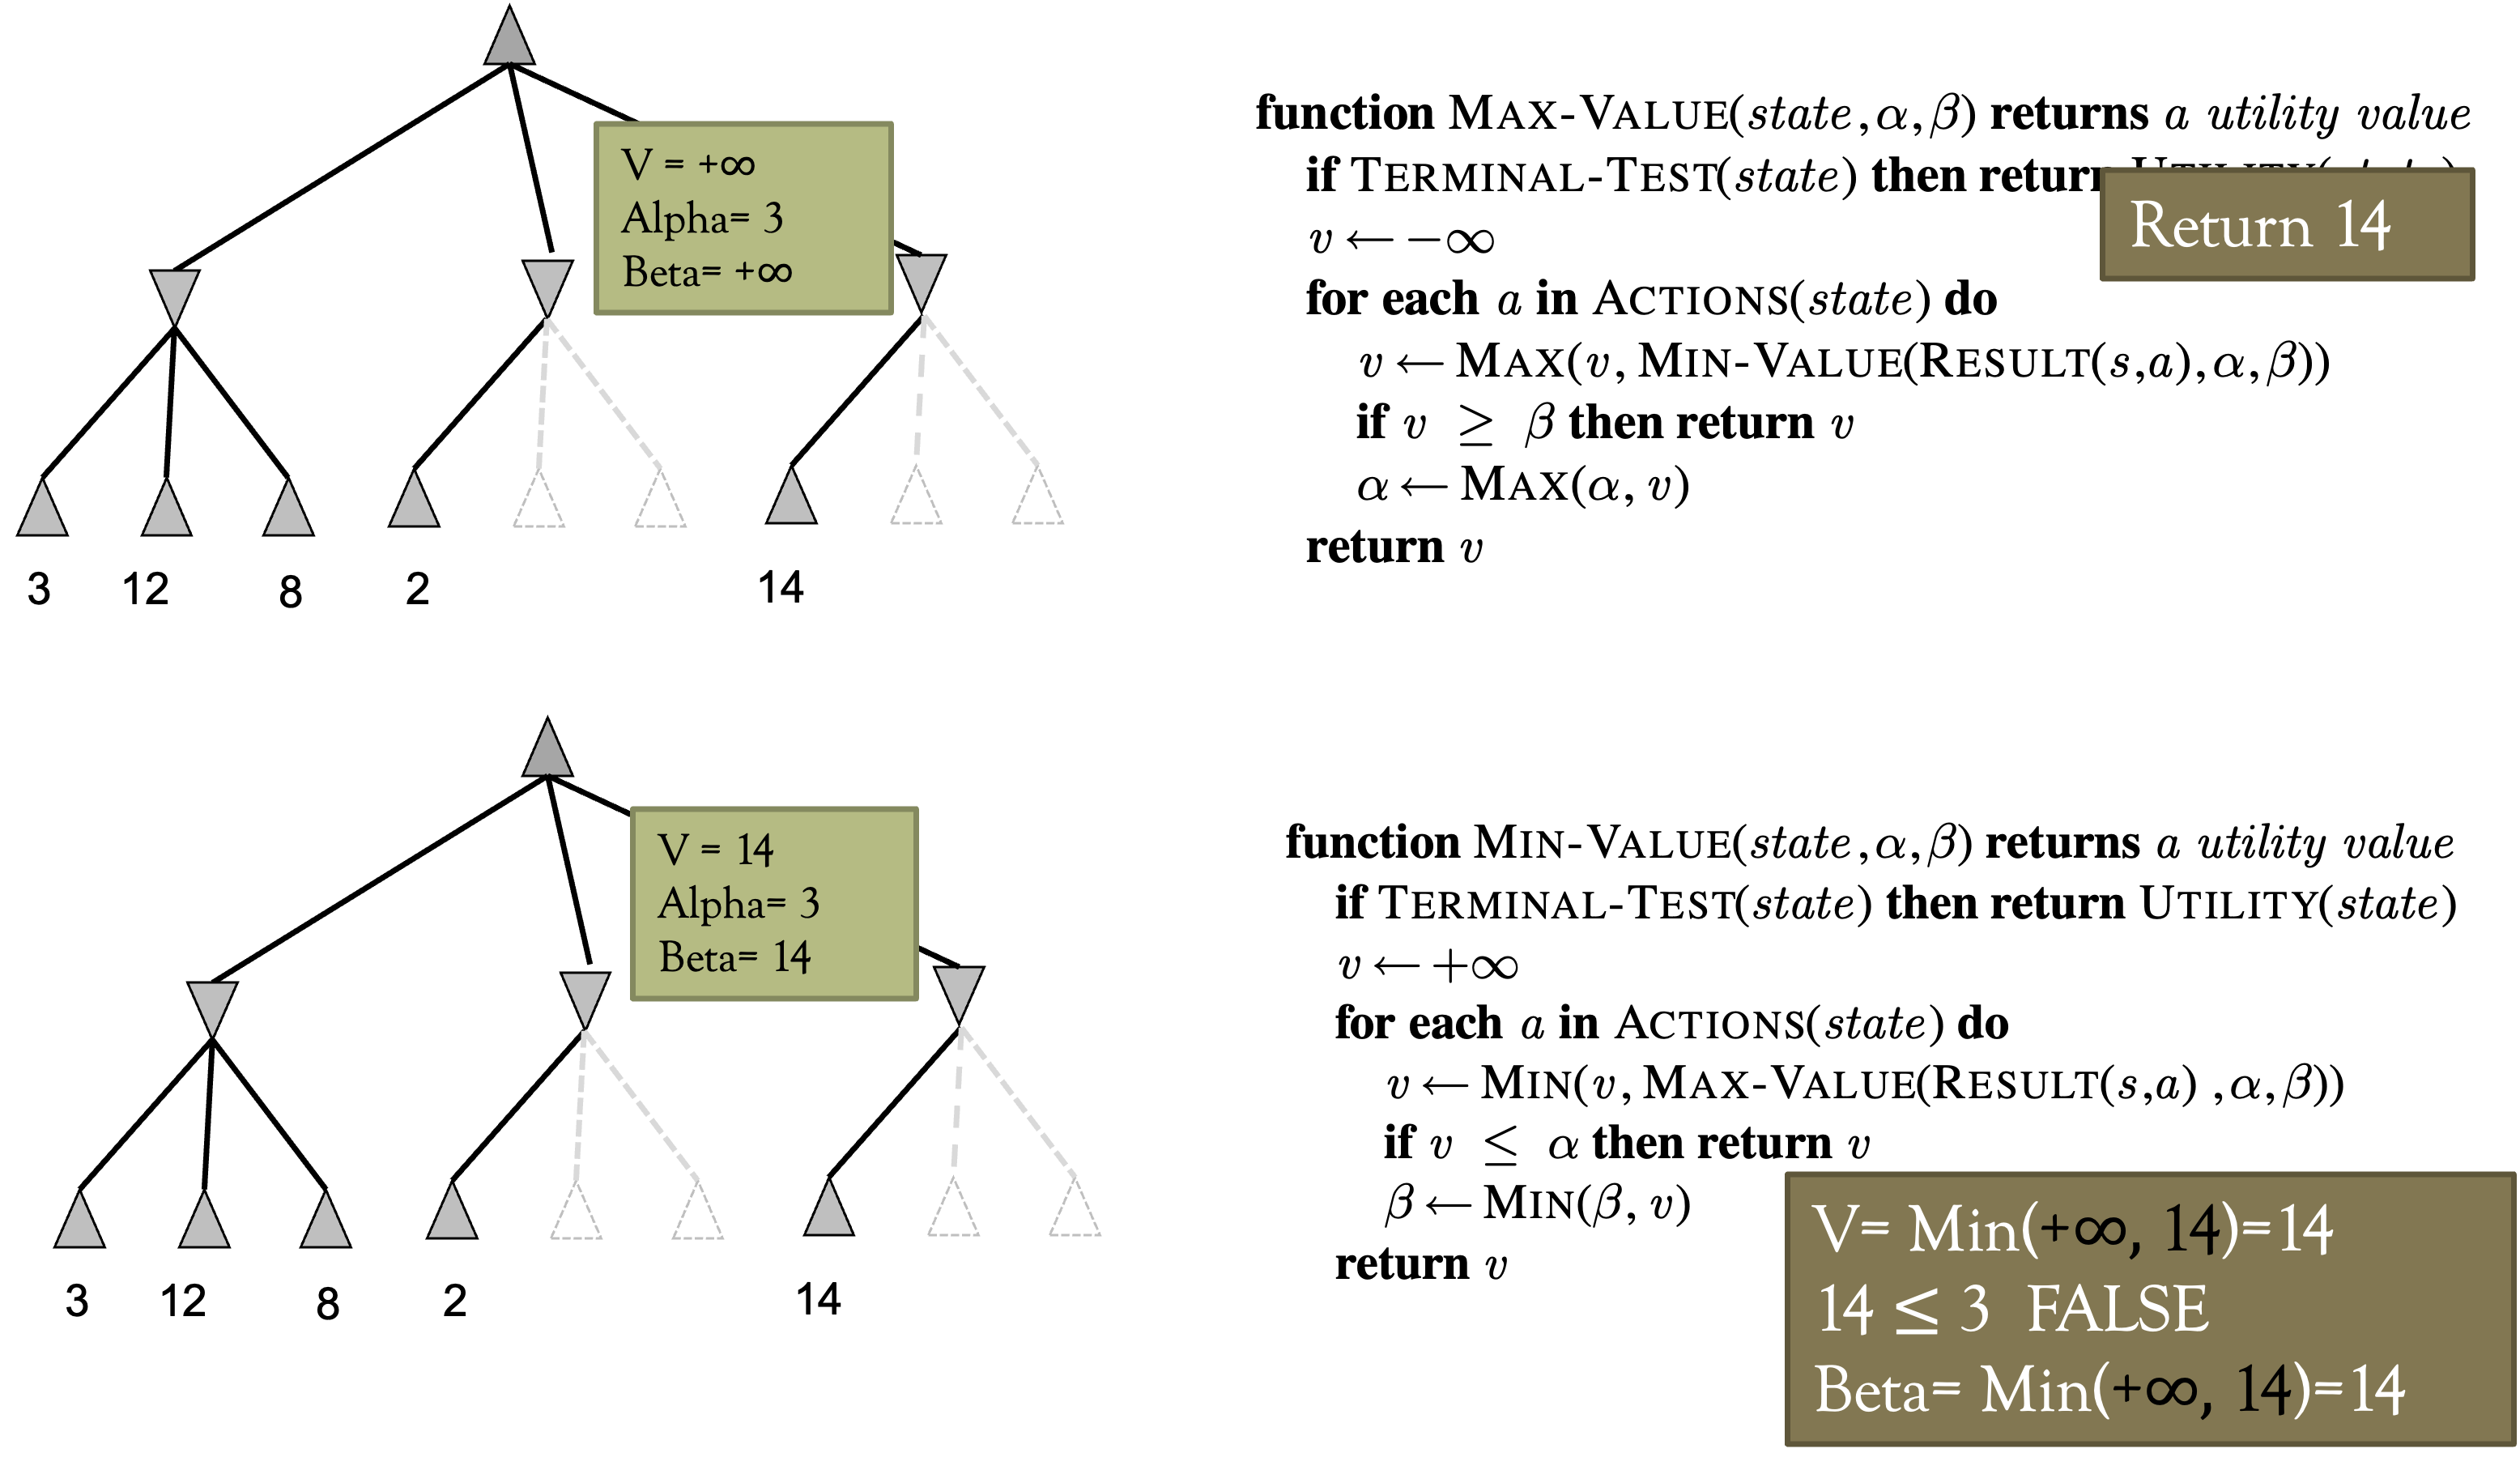
\includegraphics[scale=0.4]{./img/ejemploAlfabeta6}
\end{figure}
\end{frame} 

%%%%%%%%%%%%%%%%%%%%%%%%%%%%%%%%

\begin{frame} \frametitle{Ejemplo Poda $\alpha$-$\beta$ } \small

\begin{figure}
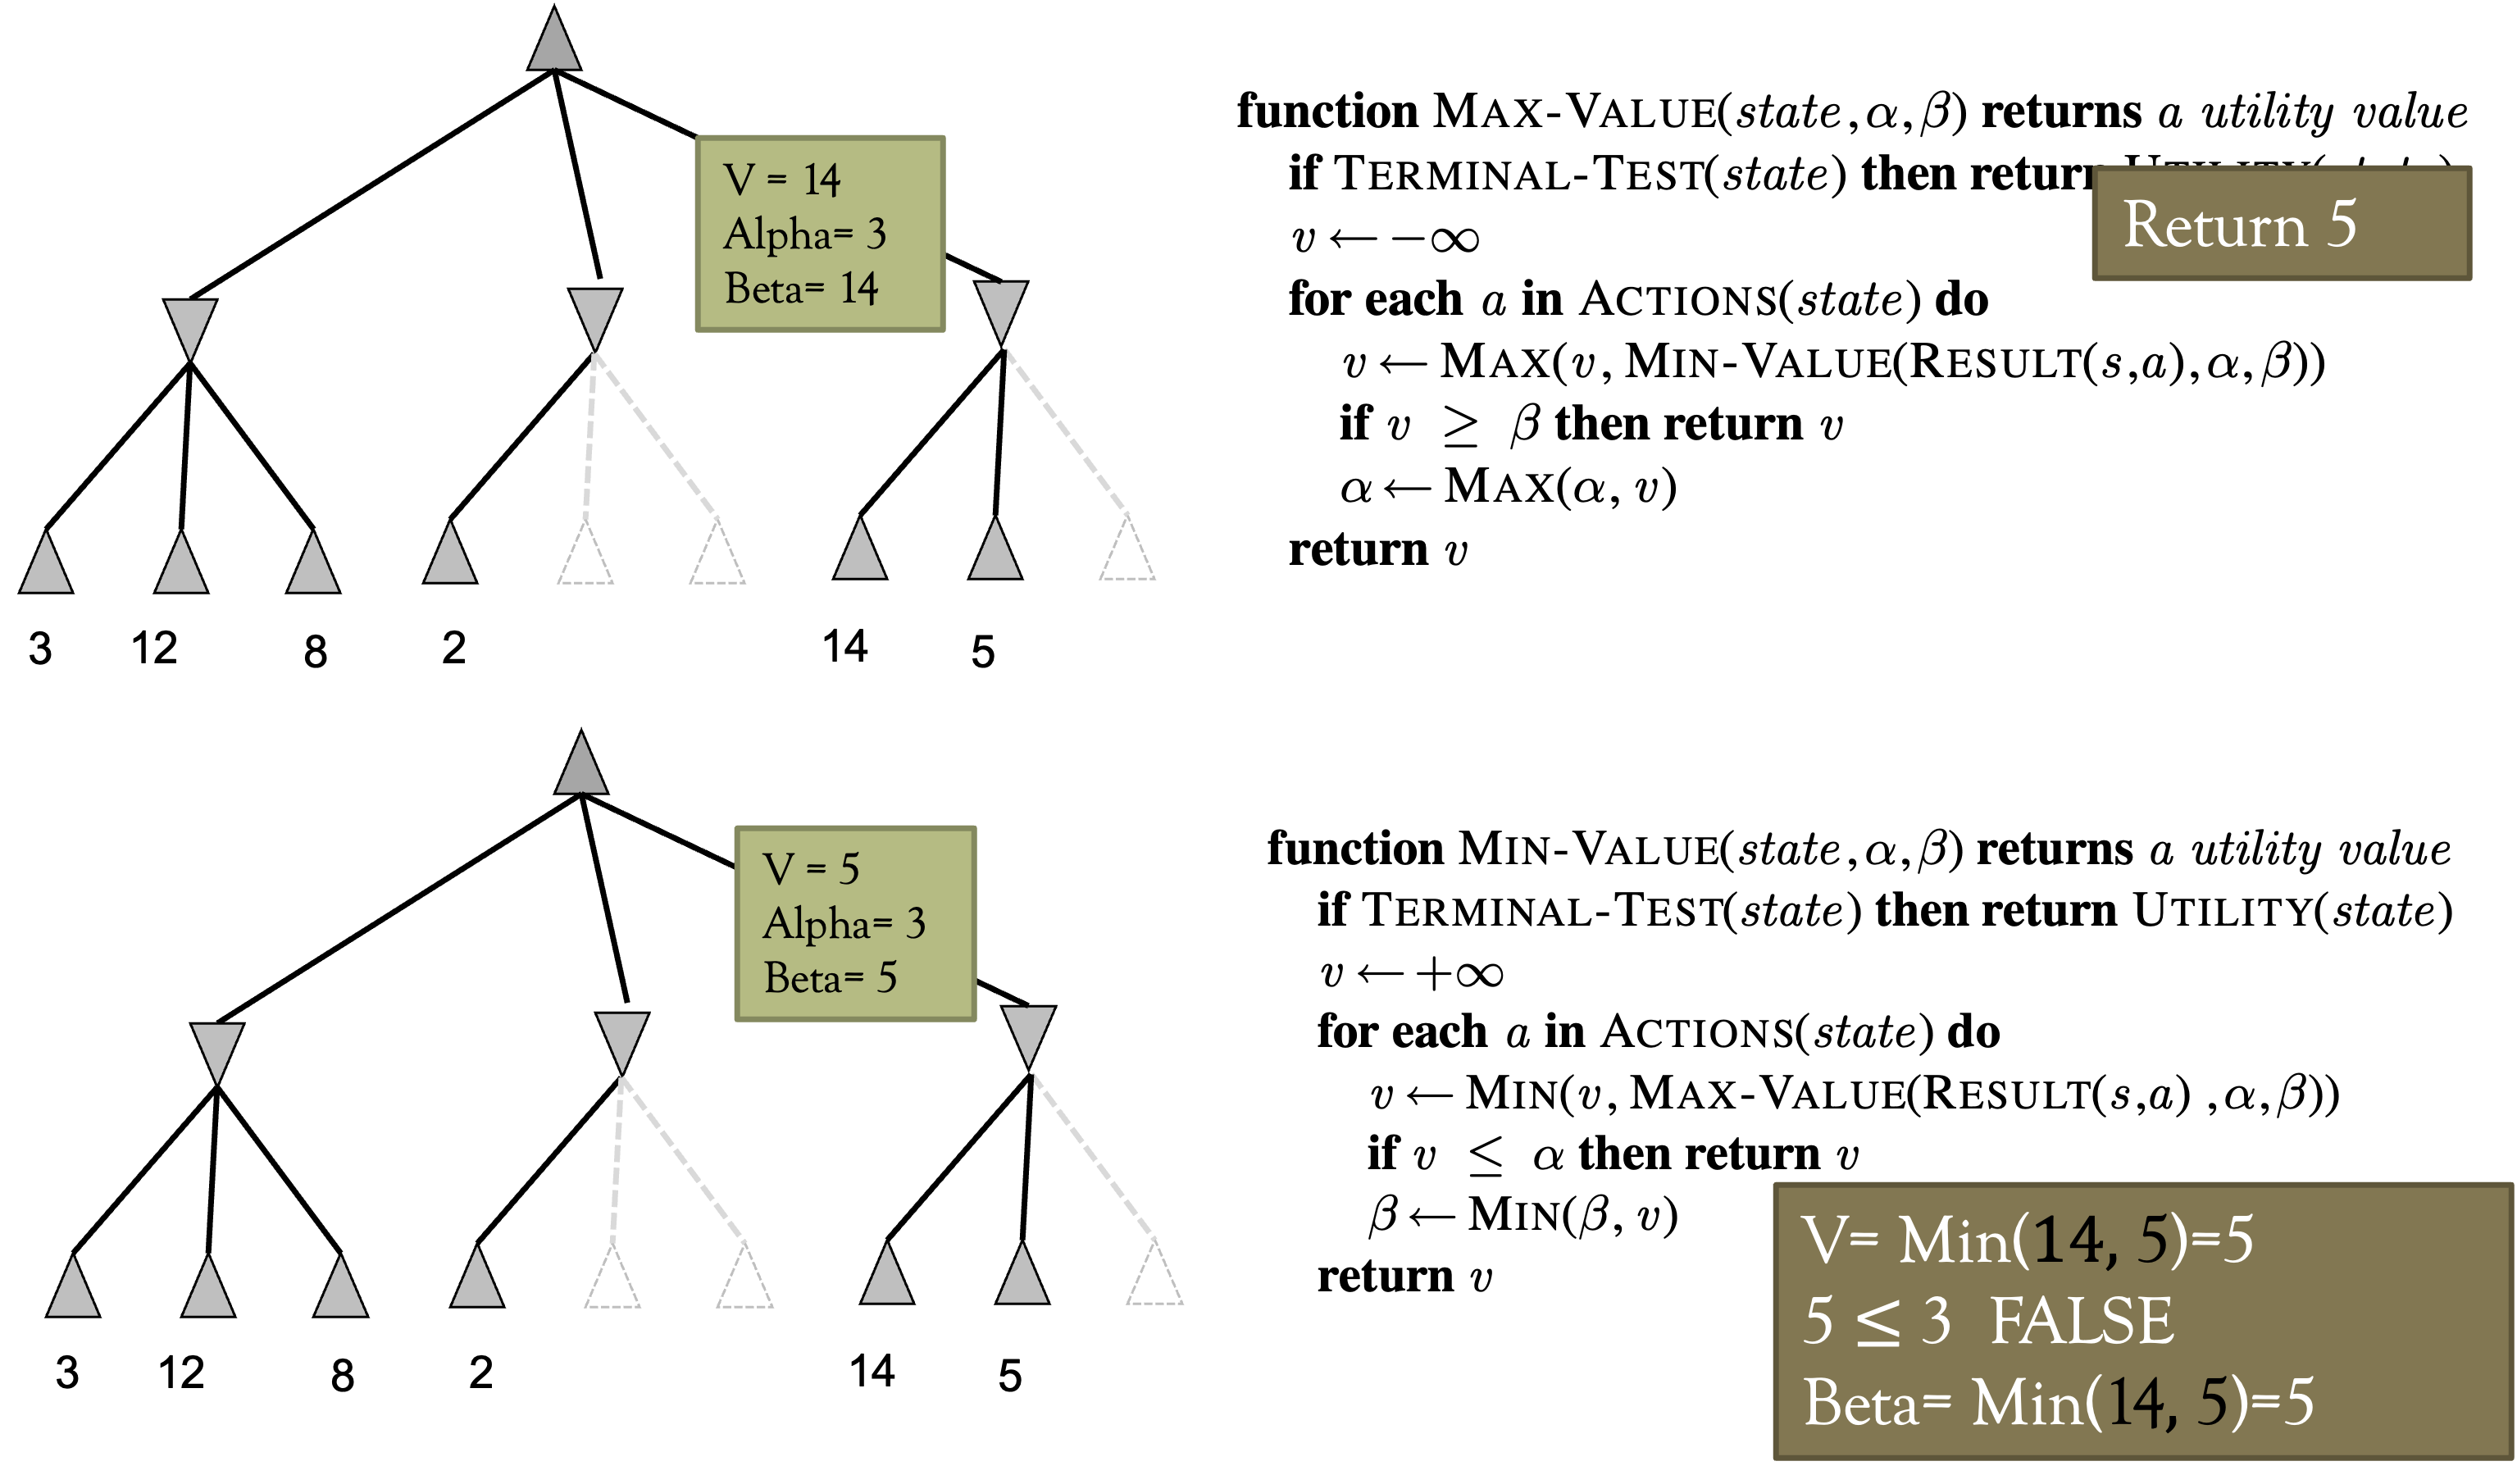
\includegraphics[scale=0.4]{./img/ejemploAlfabeta7}
\end{figure}
\end{frame} 

%%%%%%%%%%%%%%%%%%%%%%%%%%%%%%%%

\begin{frame} \frametitle{Ejemplo Poda $\alpha$-$\beta$ } \small

\begin{figure}
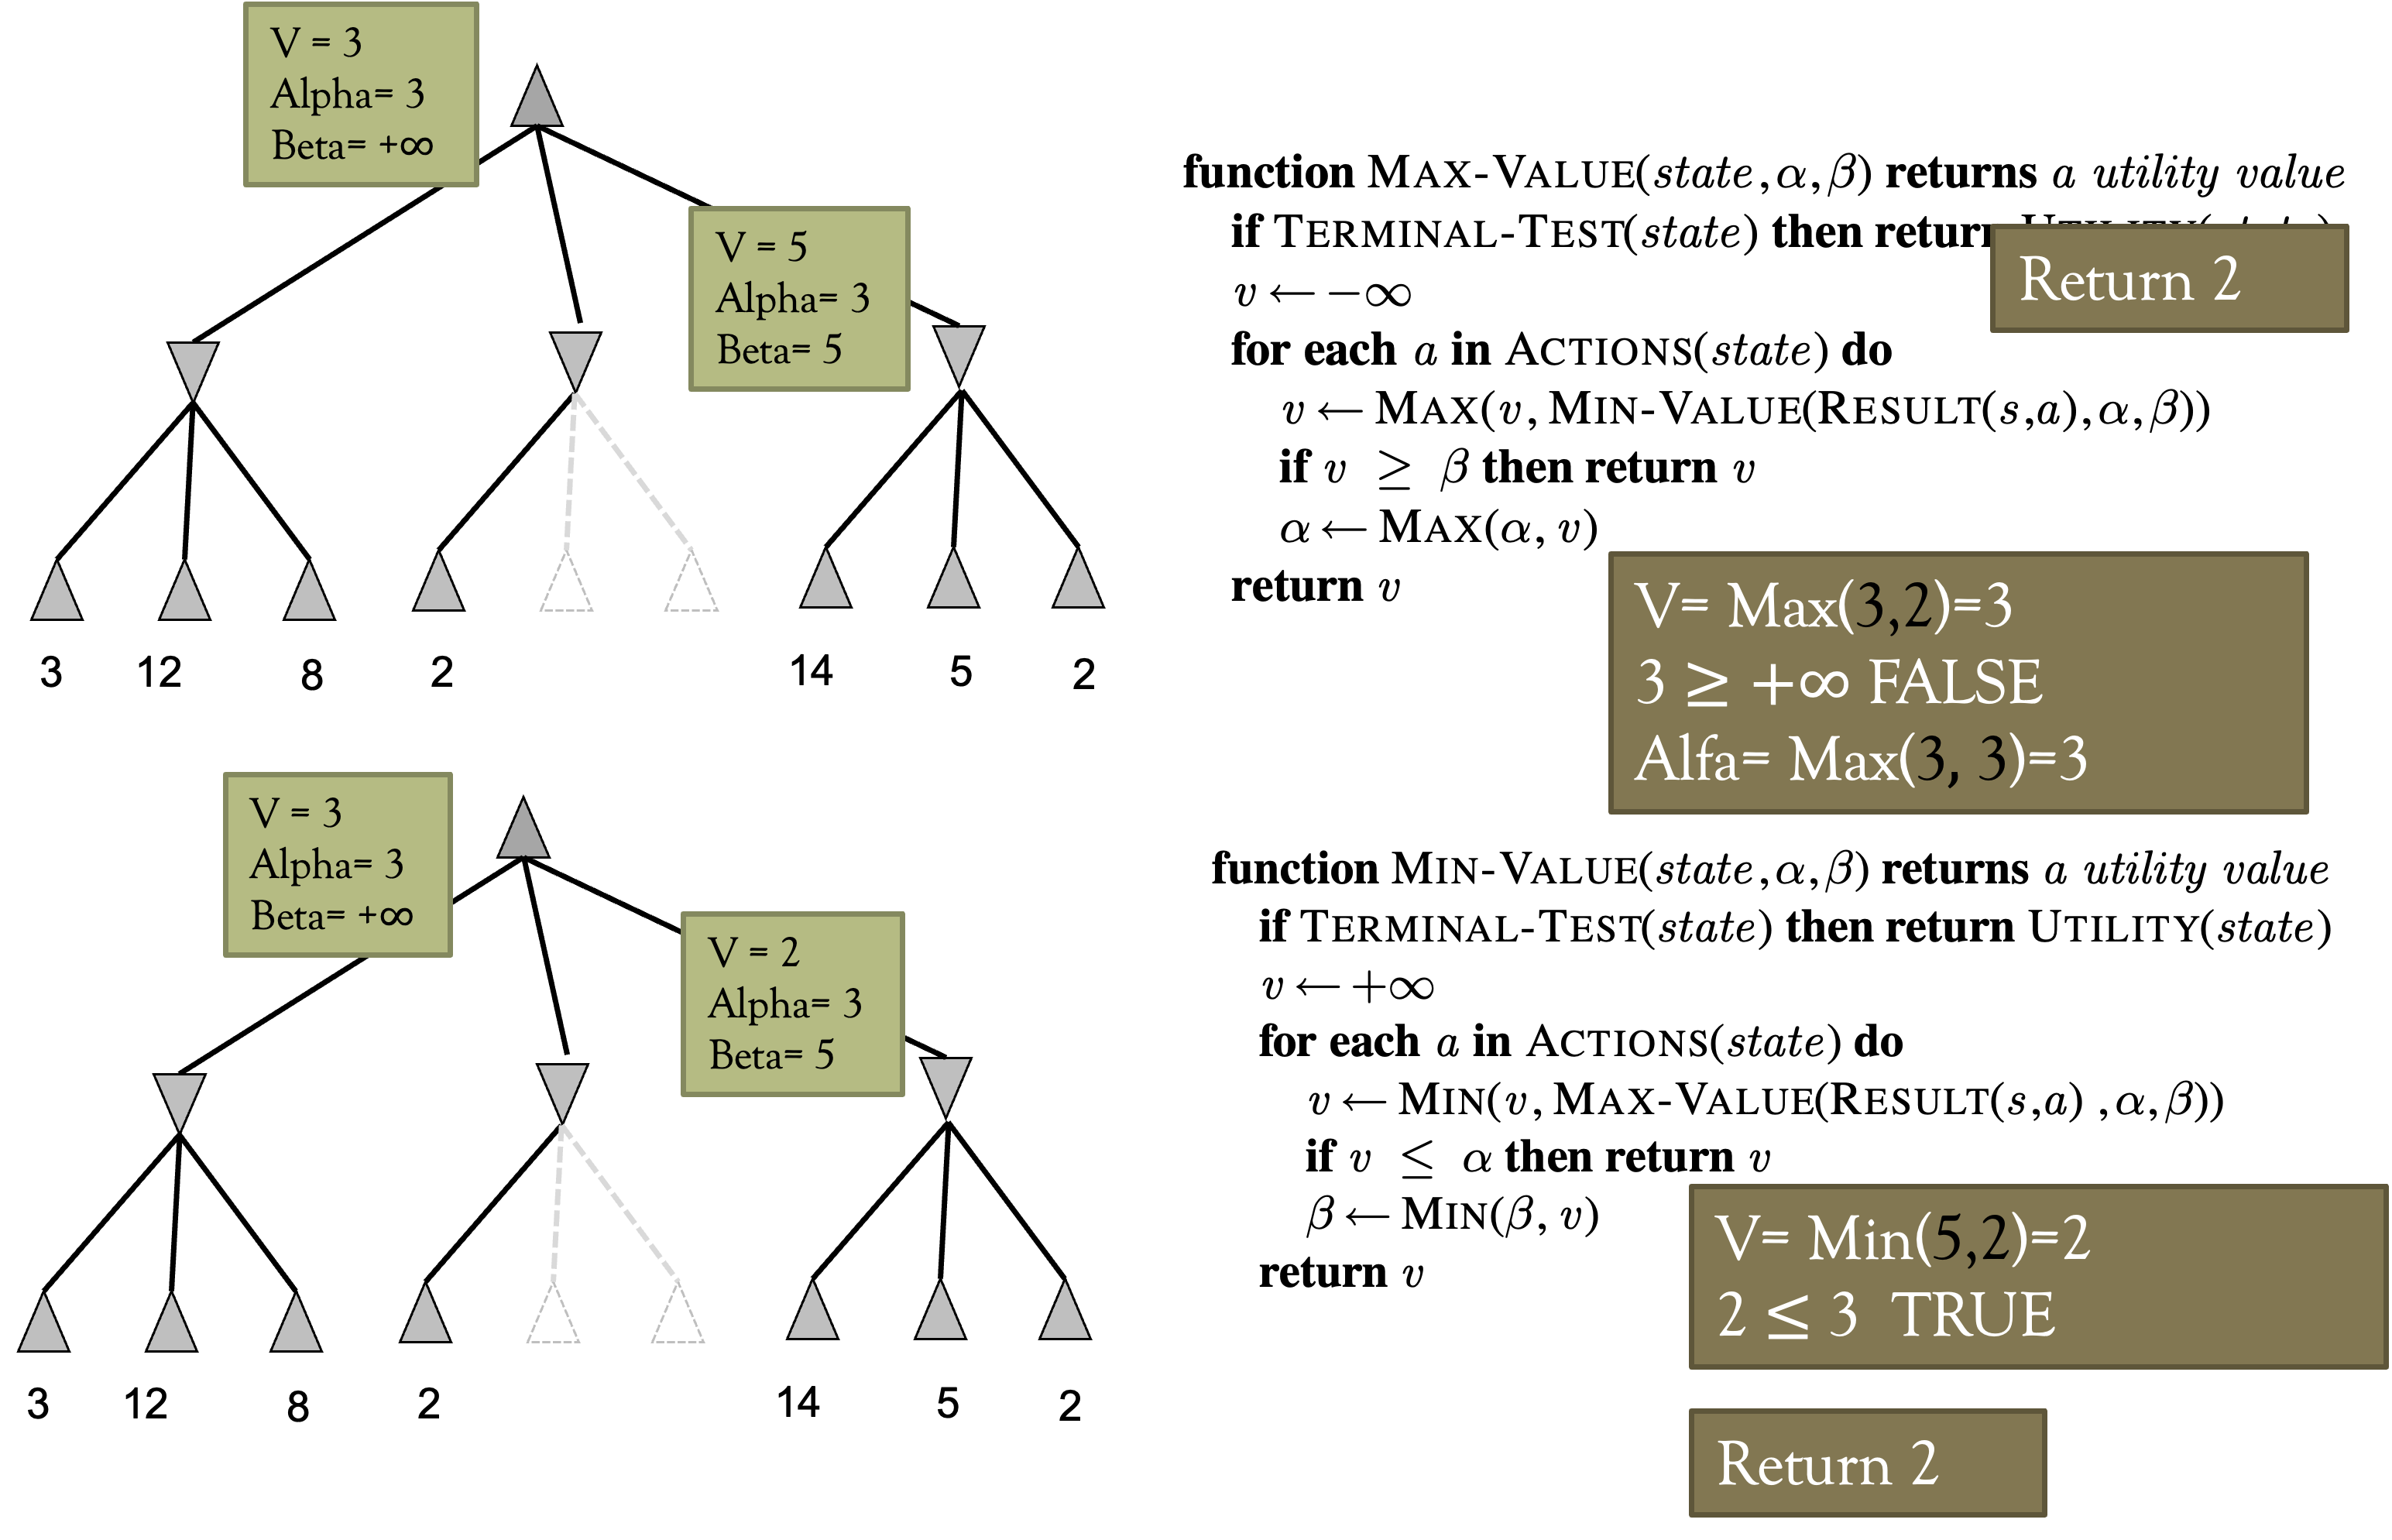
\includegraphics[scale=0.4]{./img/ejemploAlfabeta8}
\end{figure}
\end{frame} 


%%%%%%%%%%%%%%%%%%%%%%%%%%%%%%%%

\begin{frame} \frametitle{Orden de los nodos Poda $\alpha$-$\beta$ } \small
¿Cúantos nodos podemos podar?

\begin{figure}
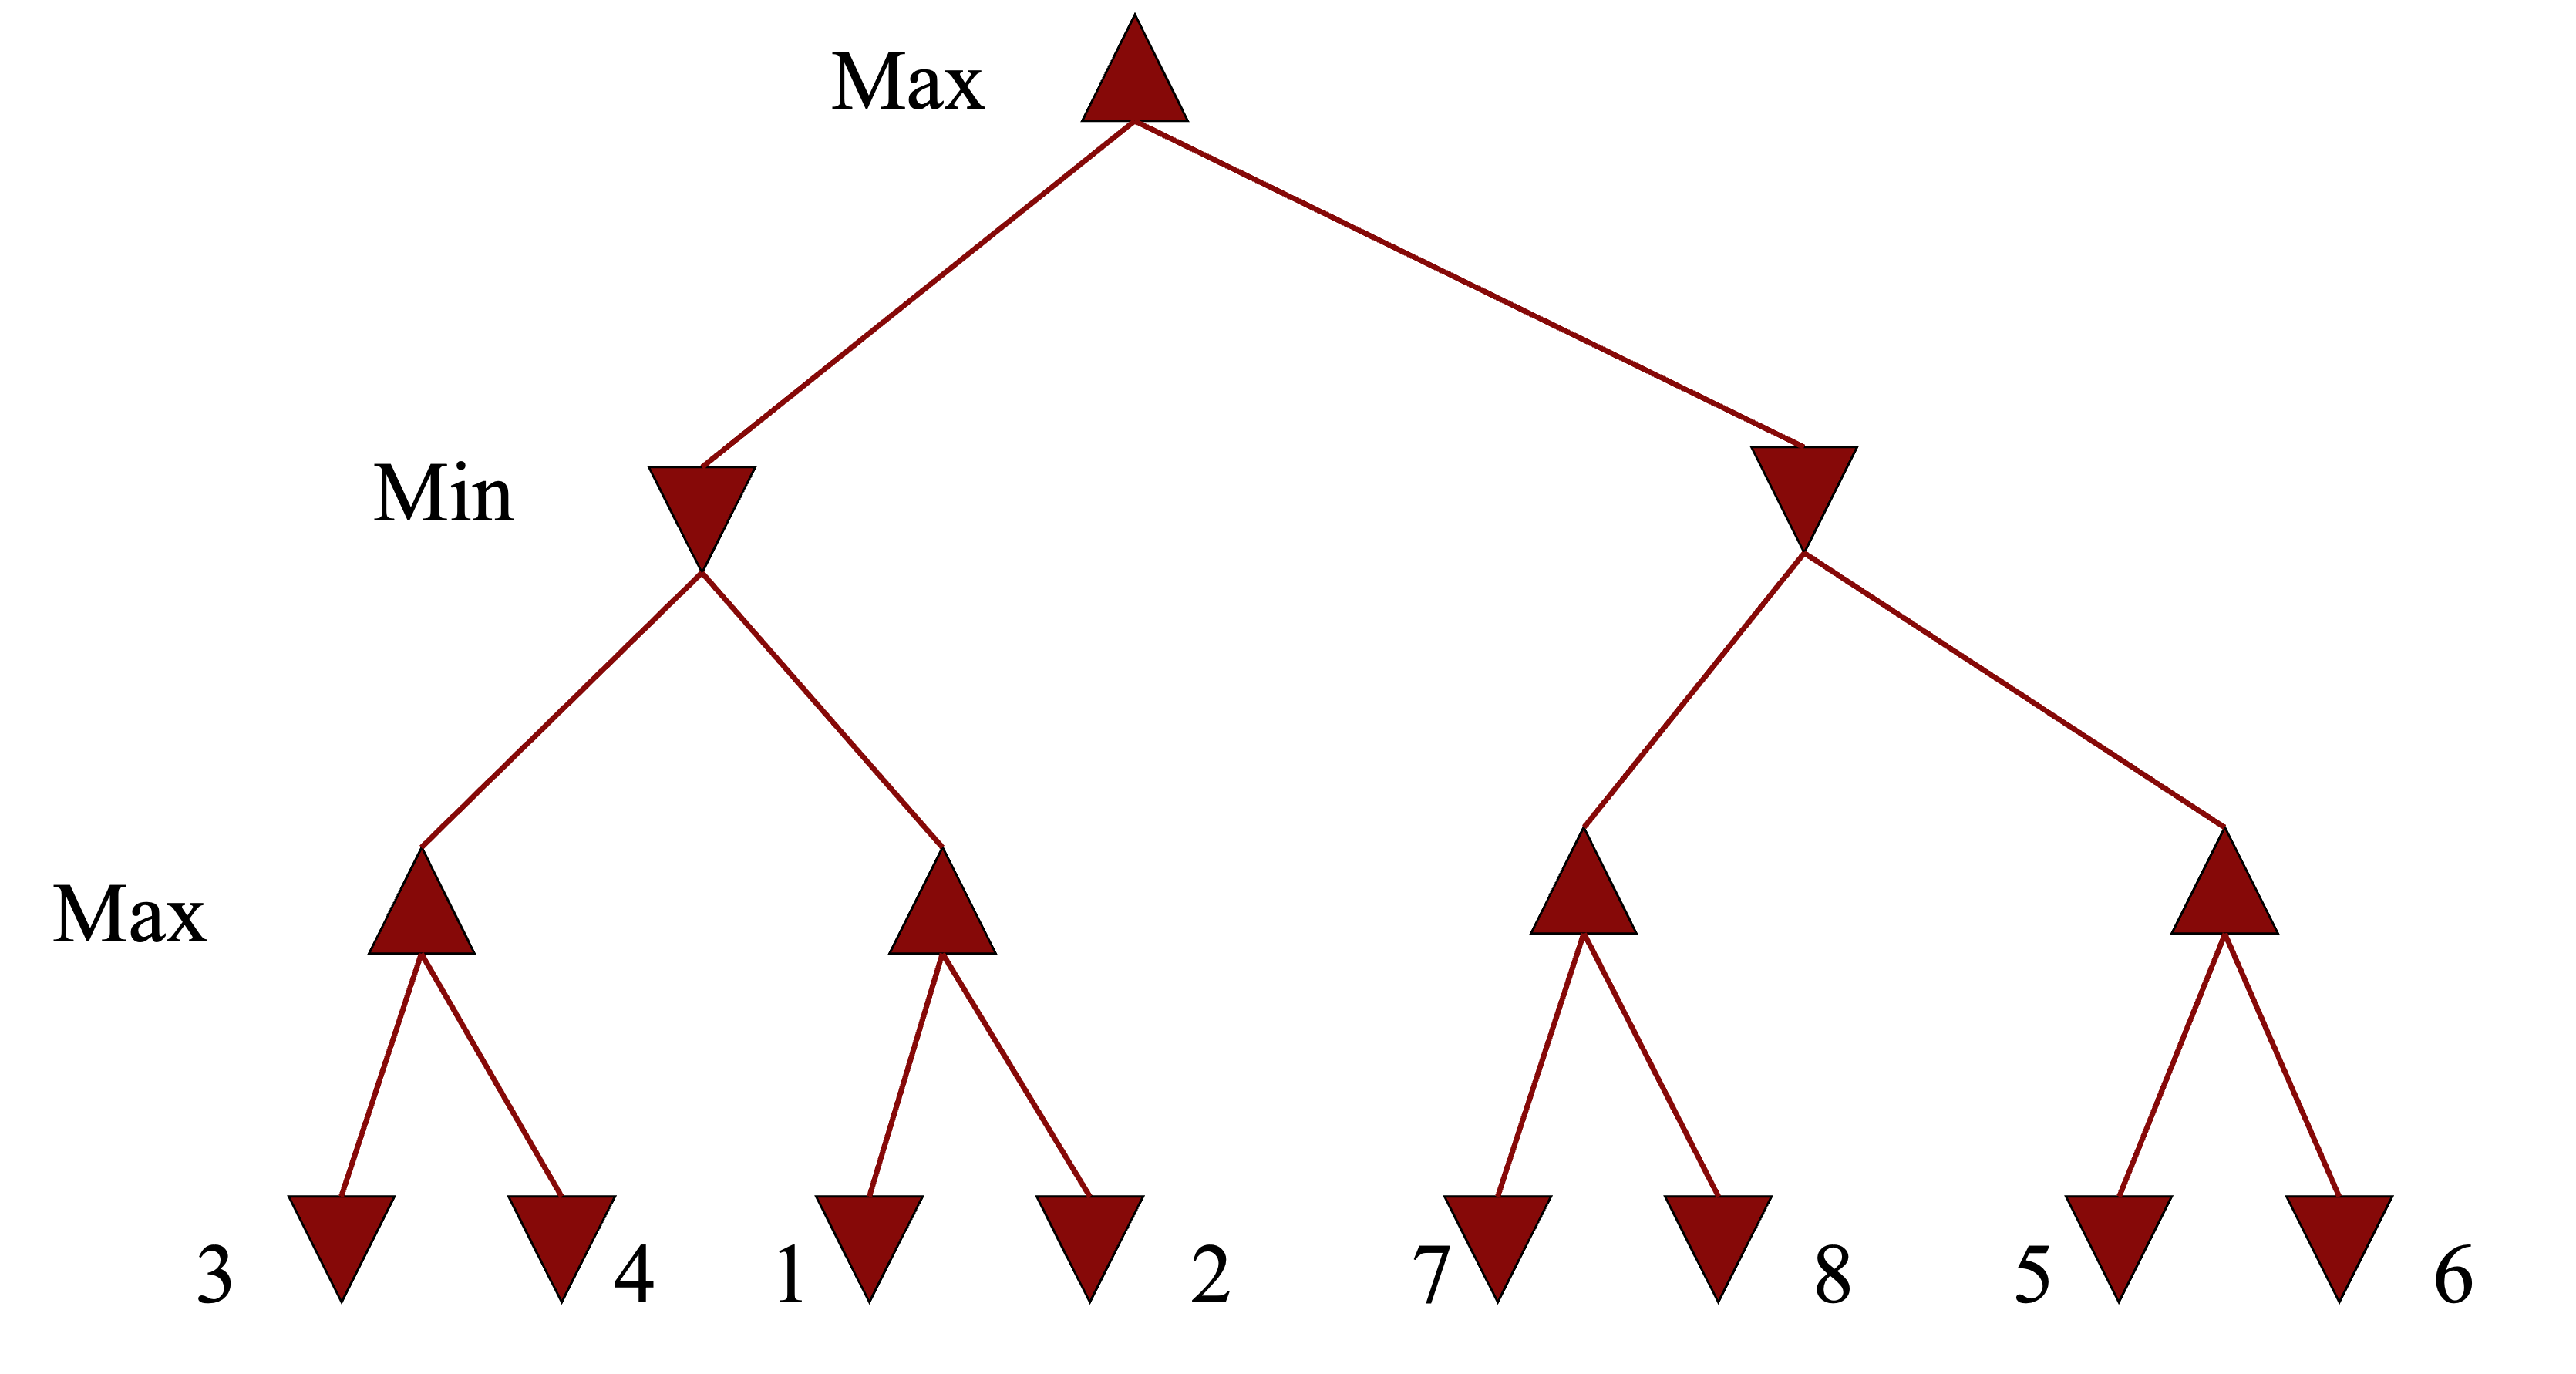
\includegraphics[scale=0.4]{./img/OrdenAlfaBeta}
\end{figure}
\end{frame} 

%%%%%%%%%%%%%%%%%%%%%%%%%%%%%%%%

\begin{frame} \frametitle{Orden de los nodos Poda $\alpha$-$\beta$ } \small

\begin{figure}
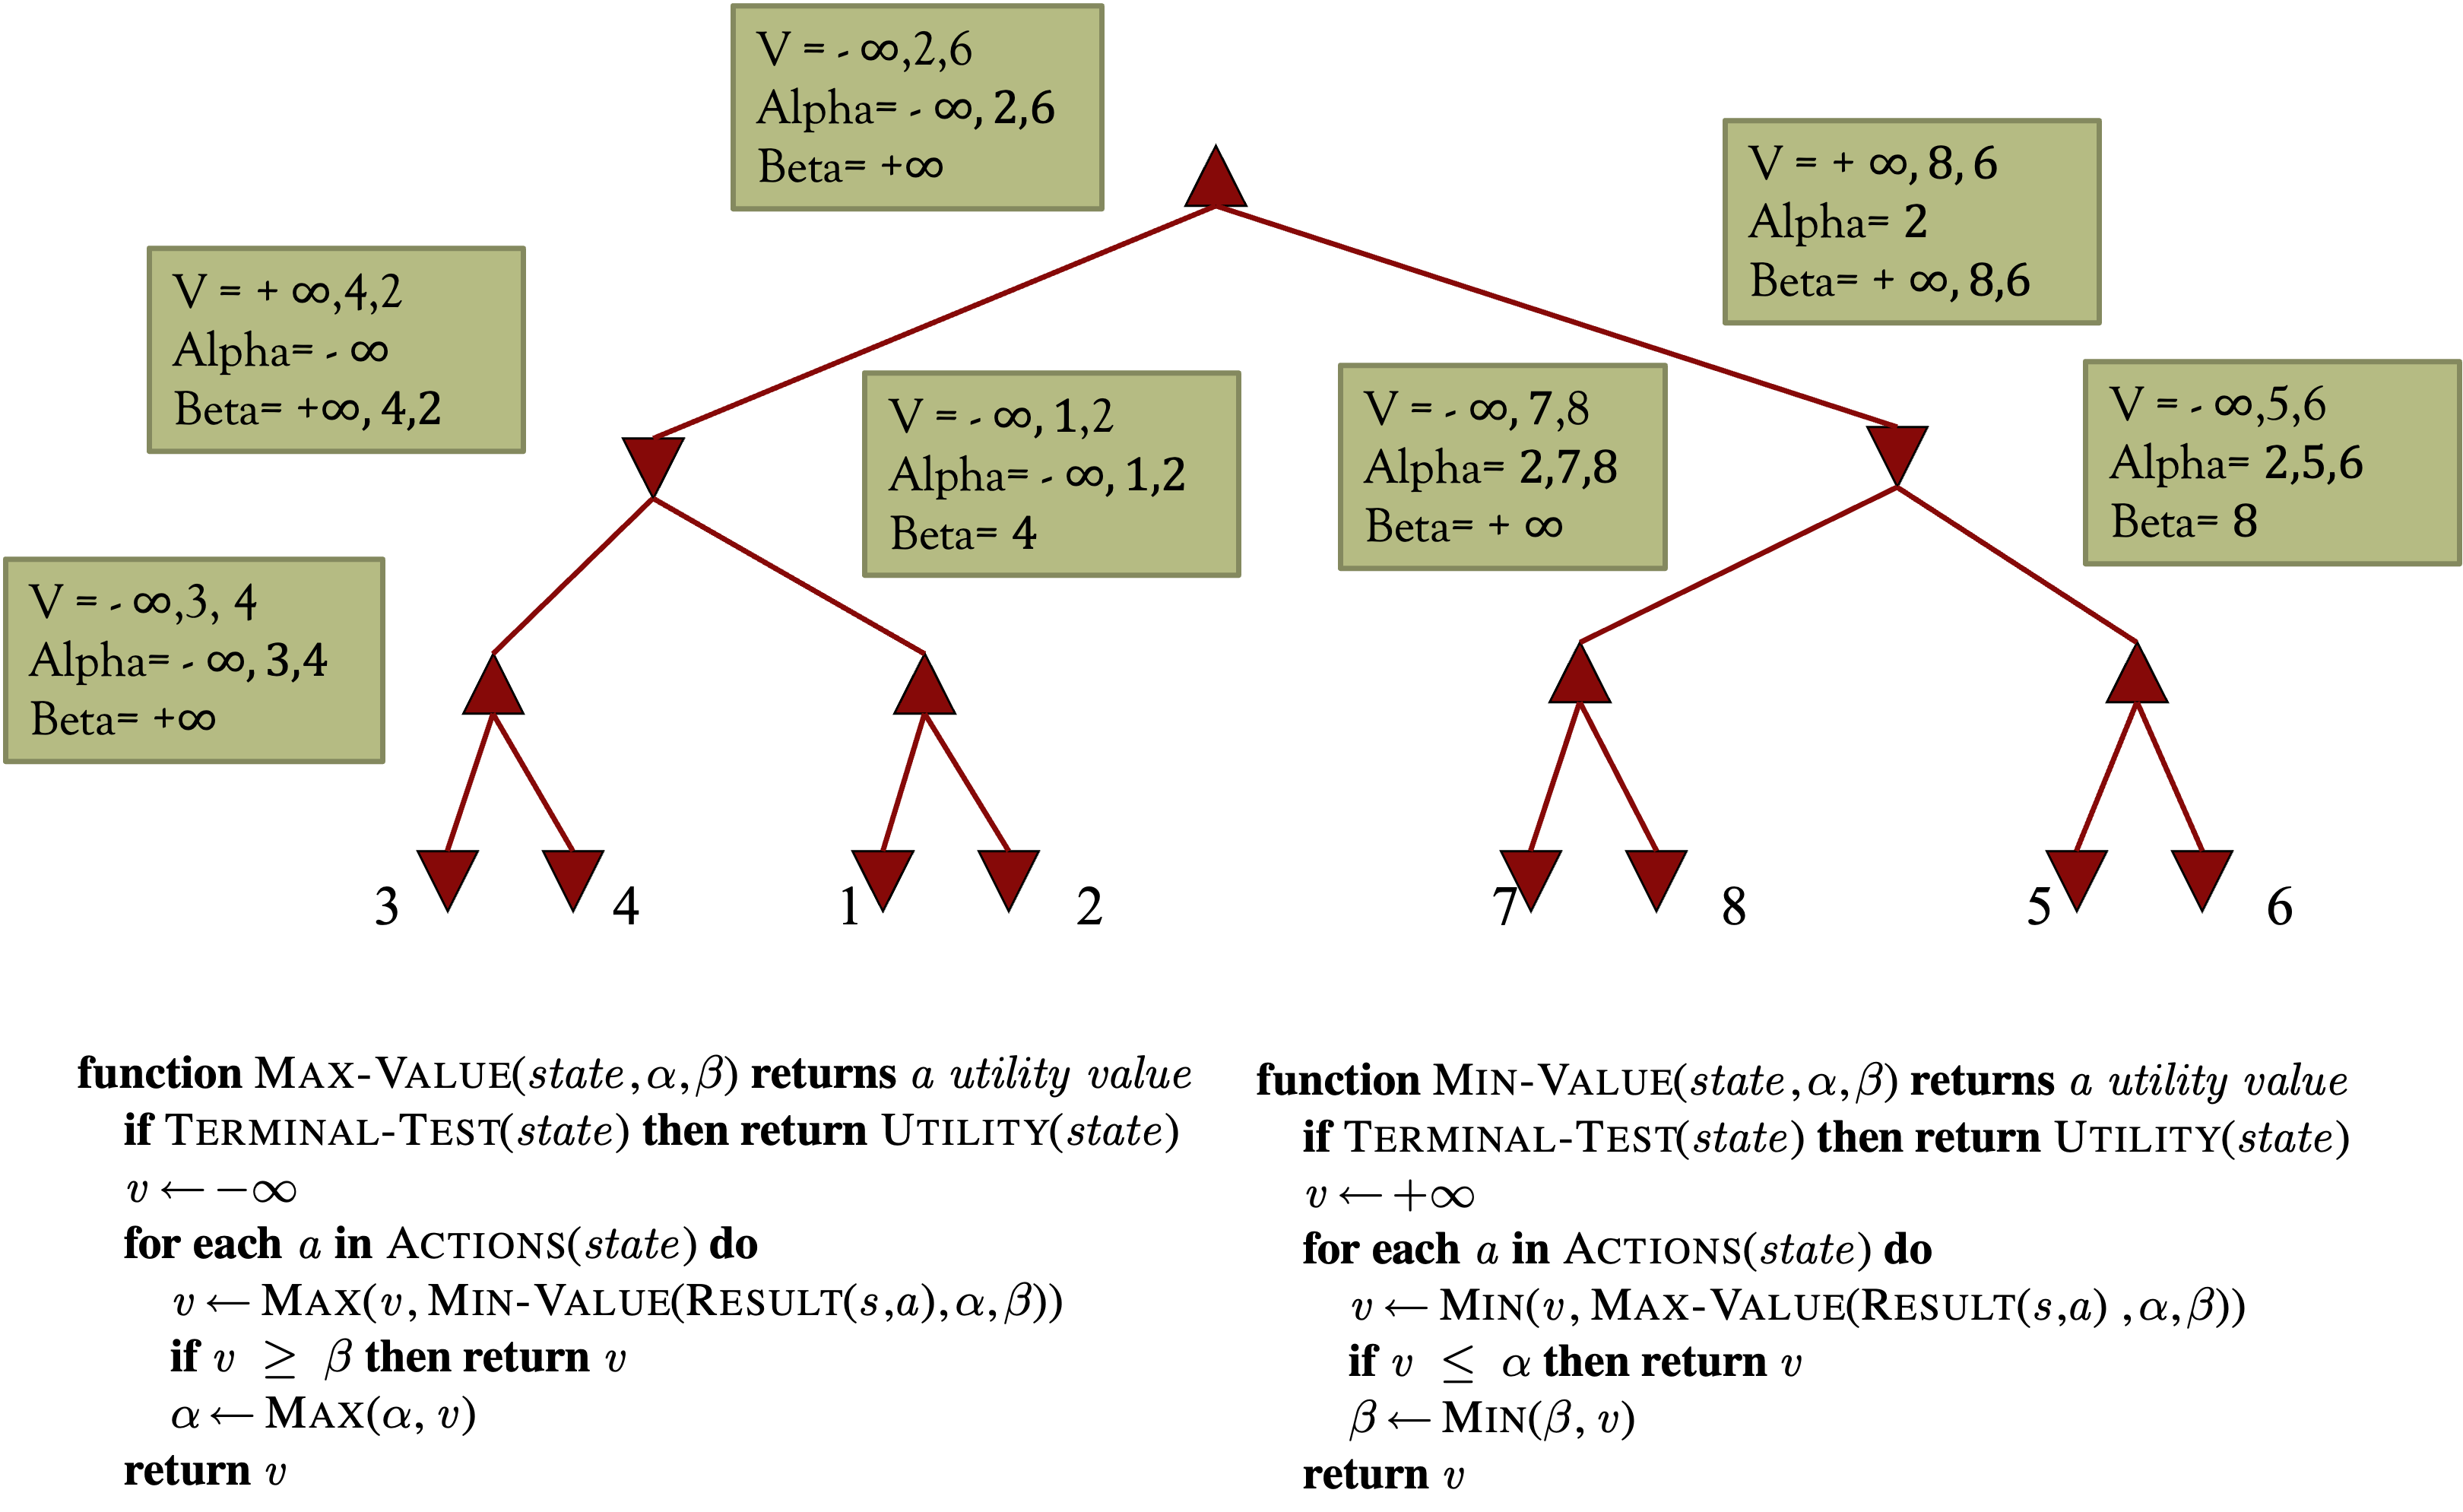
\includegraphics[scale=0.4]{./img/OrdenAlfaBeta1}
\end{figure}
\end{frame} 

%%%%%%%%%%%%%%%%%%%%%%%%%%%%%%%%

\begin{frame} \frametitle{Orden de los nodos Poda $\alpha$-$\beta$ } \small

No podemos podar ningún nodo. Los nodos favorables son los últimos en explorar.

\begin{figure}
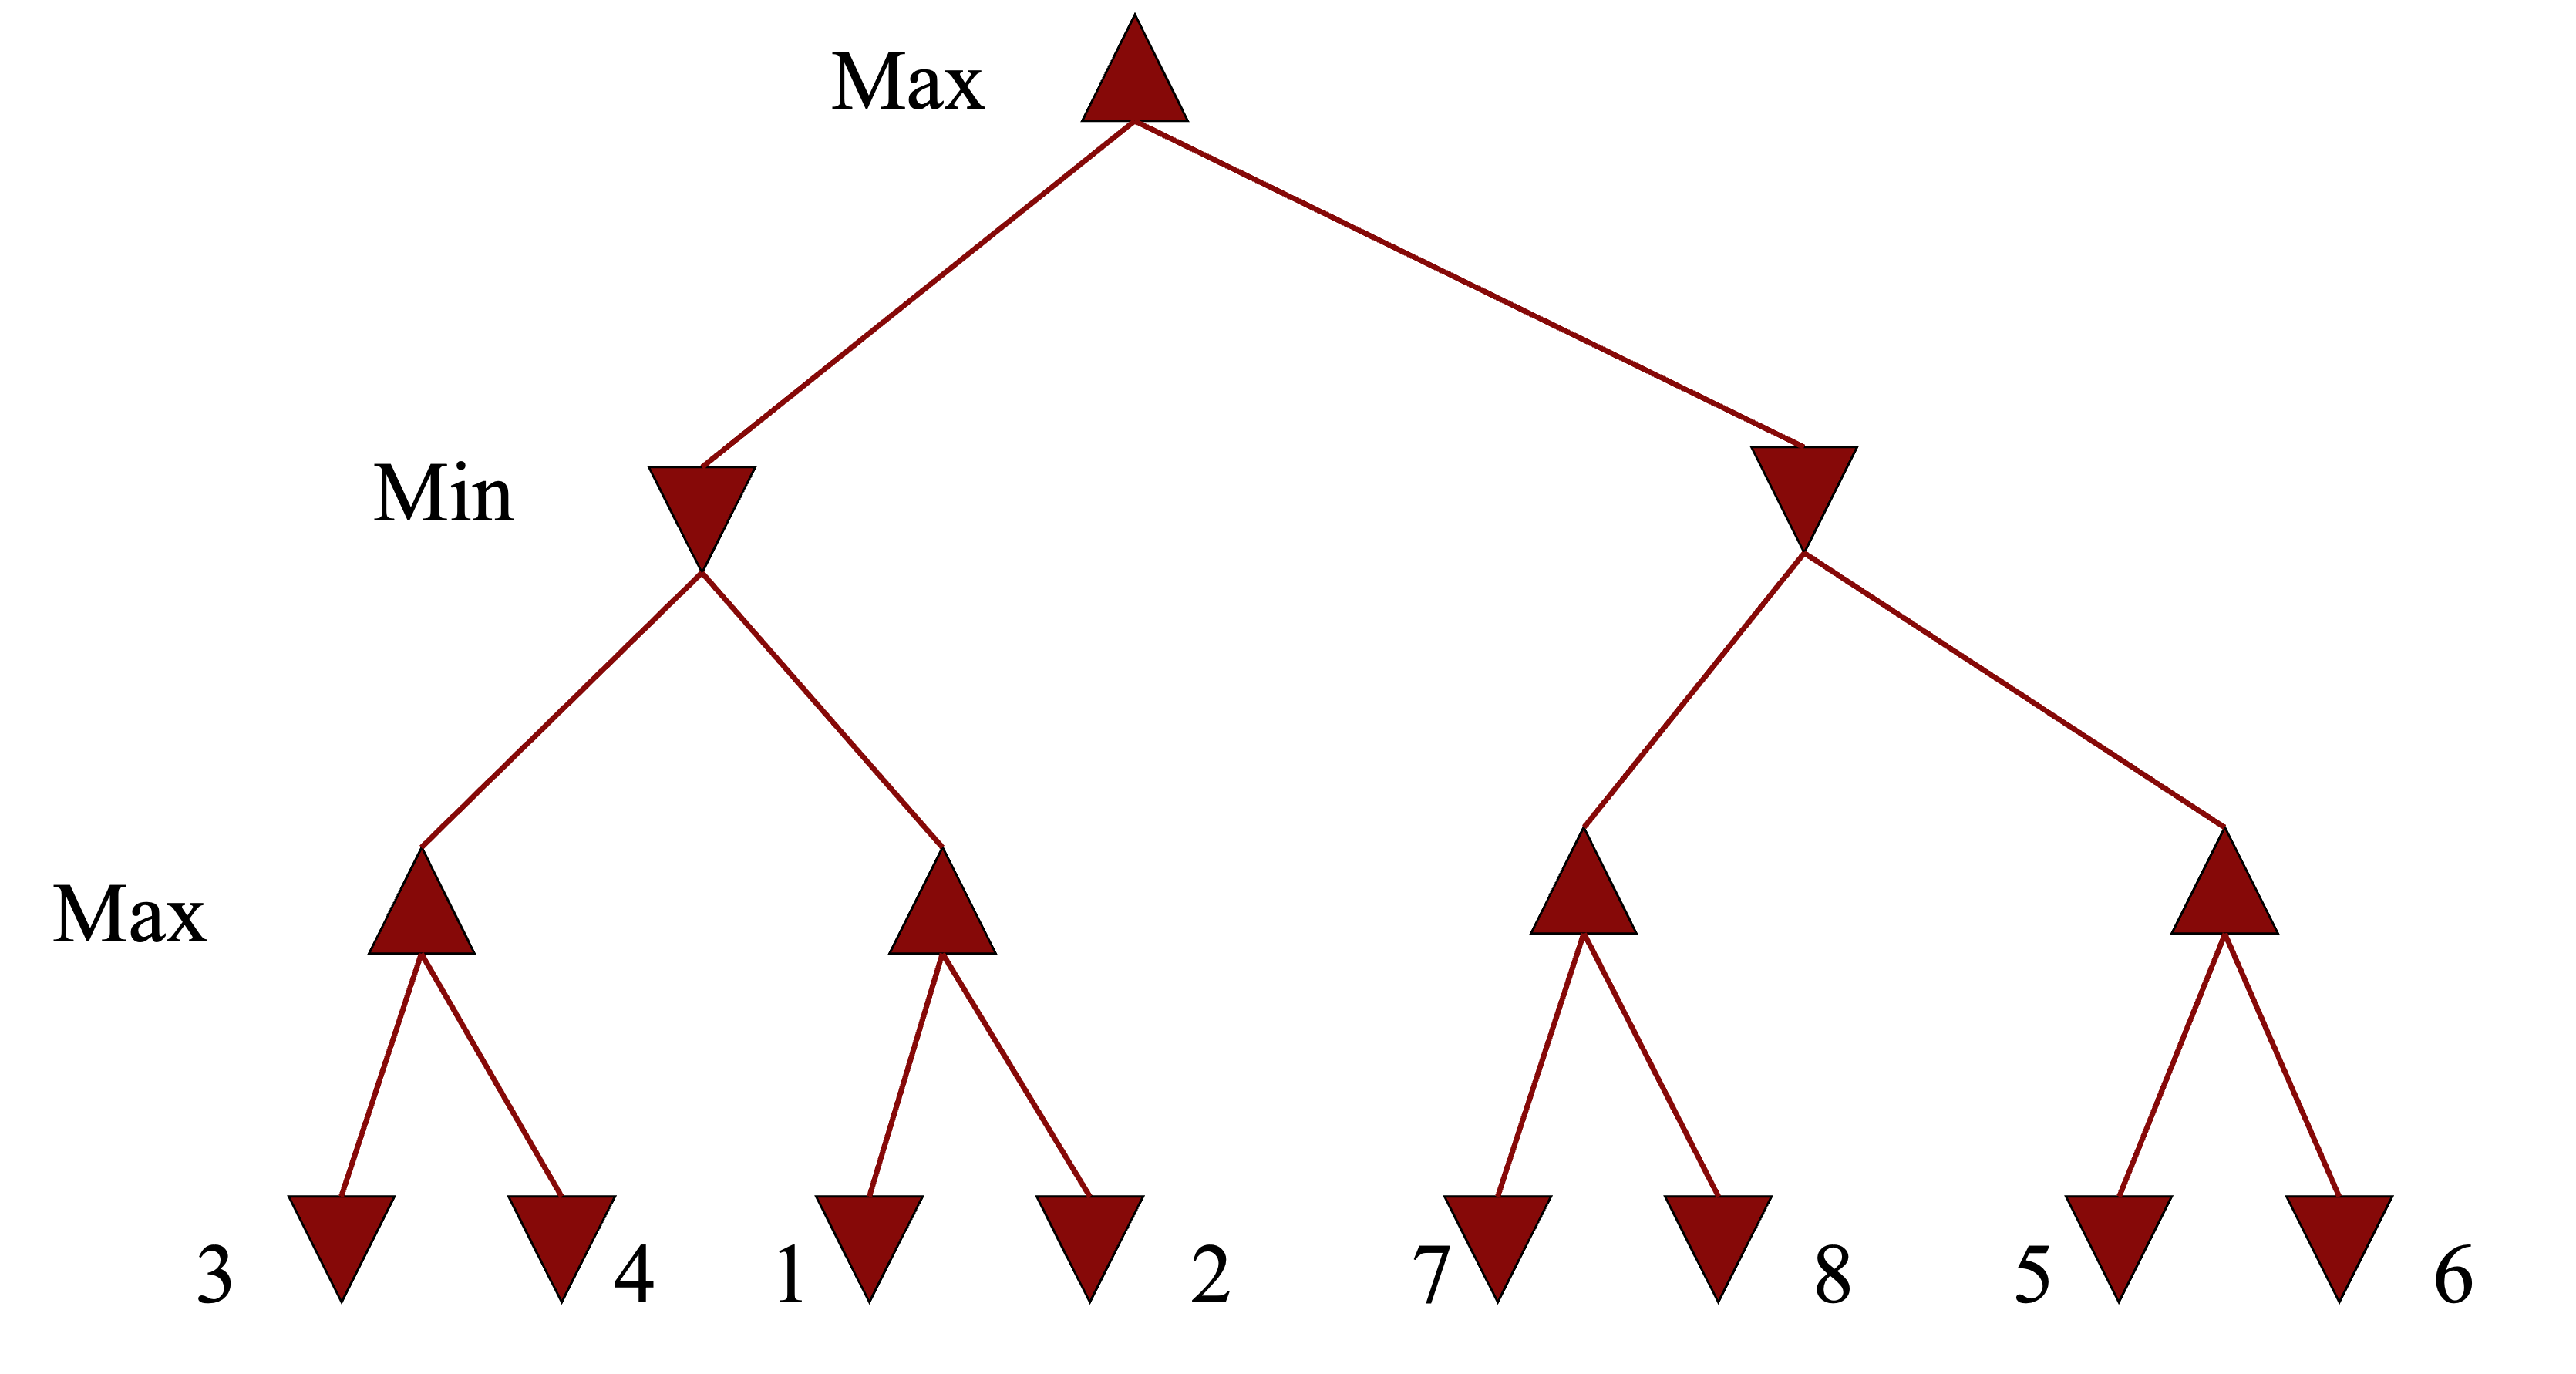
\includegraphics[scale=0.4]{./img/OrdenAlfaBeta}
\end{figure}
\end{frame} 

%%%%%%%%%%%%%%%%%%%%%%%%%%%%%%%%

\begin{frame} \frametitle{Orden de los nodos Poda $\alpha$-$\beta$ } \small

¿Cúantos nodos podemos podar?

\begin{figure}
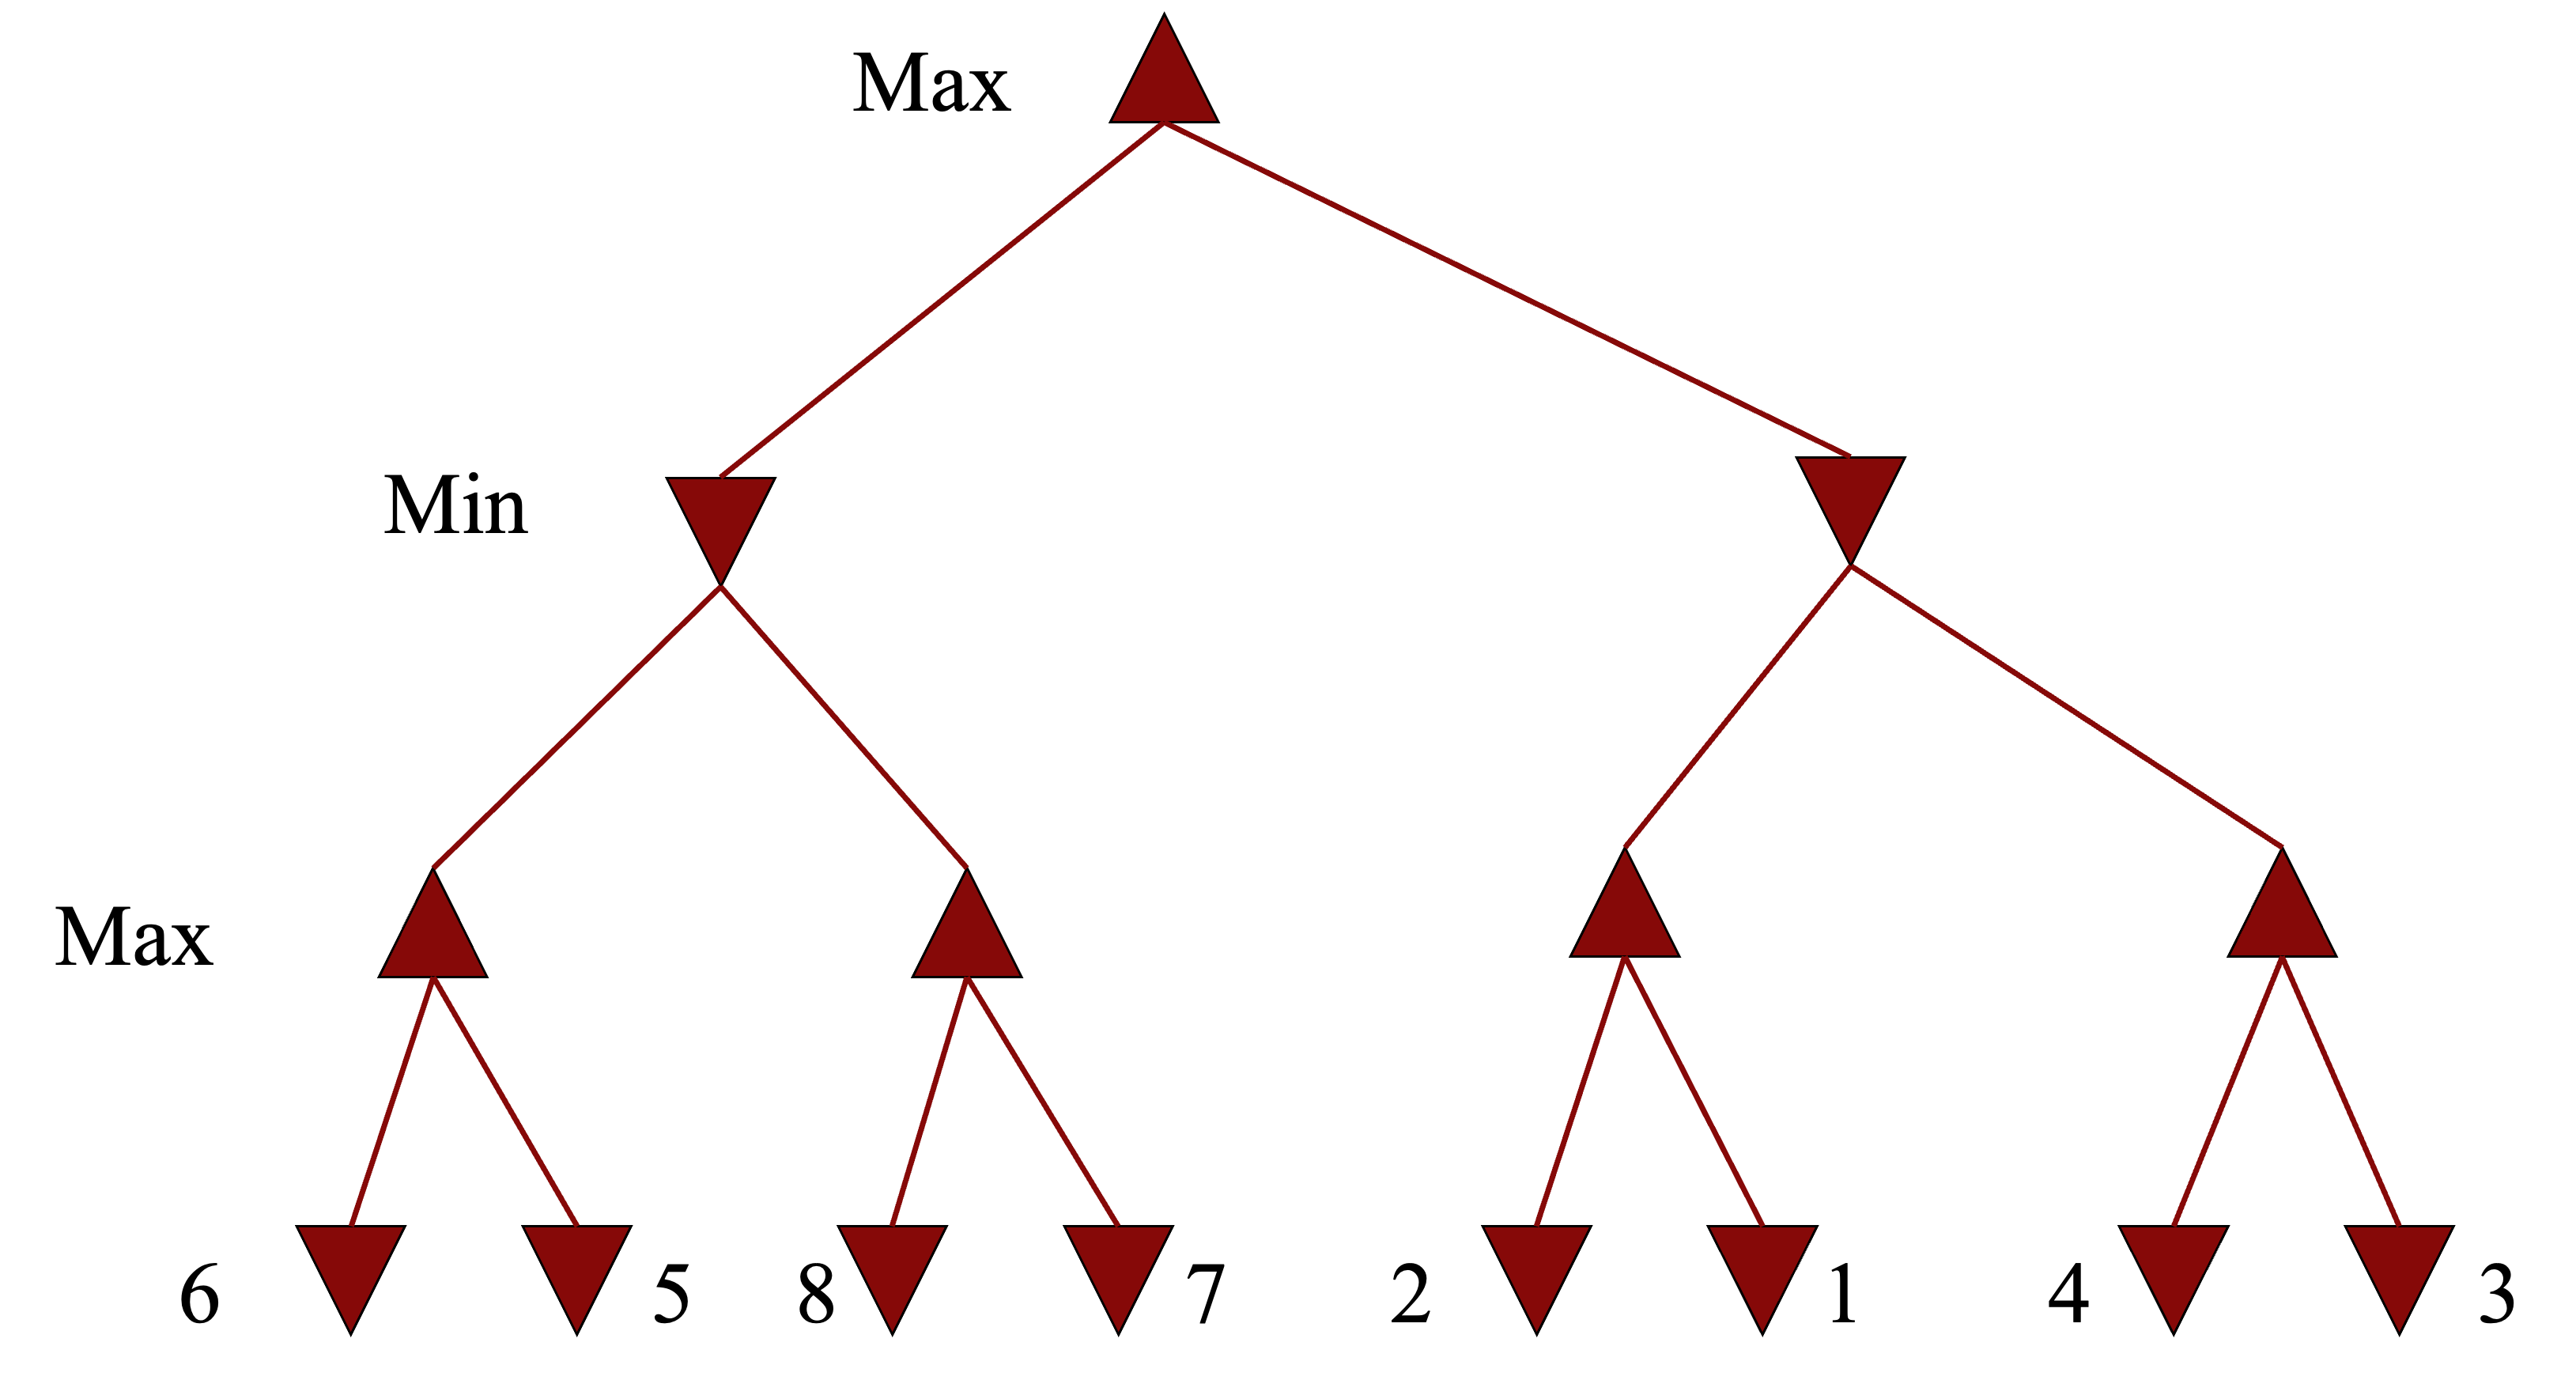
\includegraphics[scale=0.4]{./img/OrdenAlfaBeta2}
\end{figure}
\end{frame} 

%%%%%%%%%%%%%%%%%%%%%%%%%%%%%%%%

\begin{frame} \frametitle{Orden de los nodos Poda $\alpha$-$\beta$ } \small

Hemos podado 3 nodos.

\begin{figure}
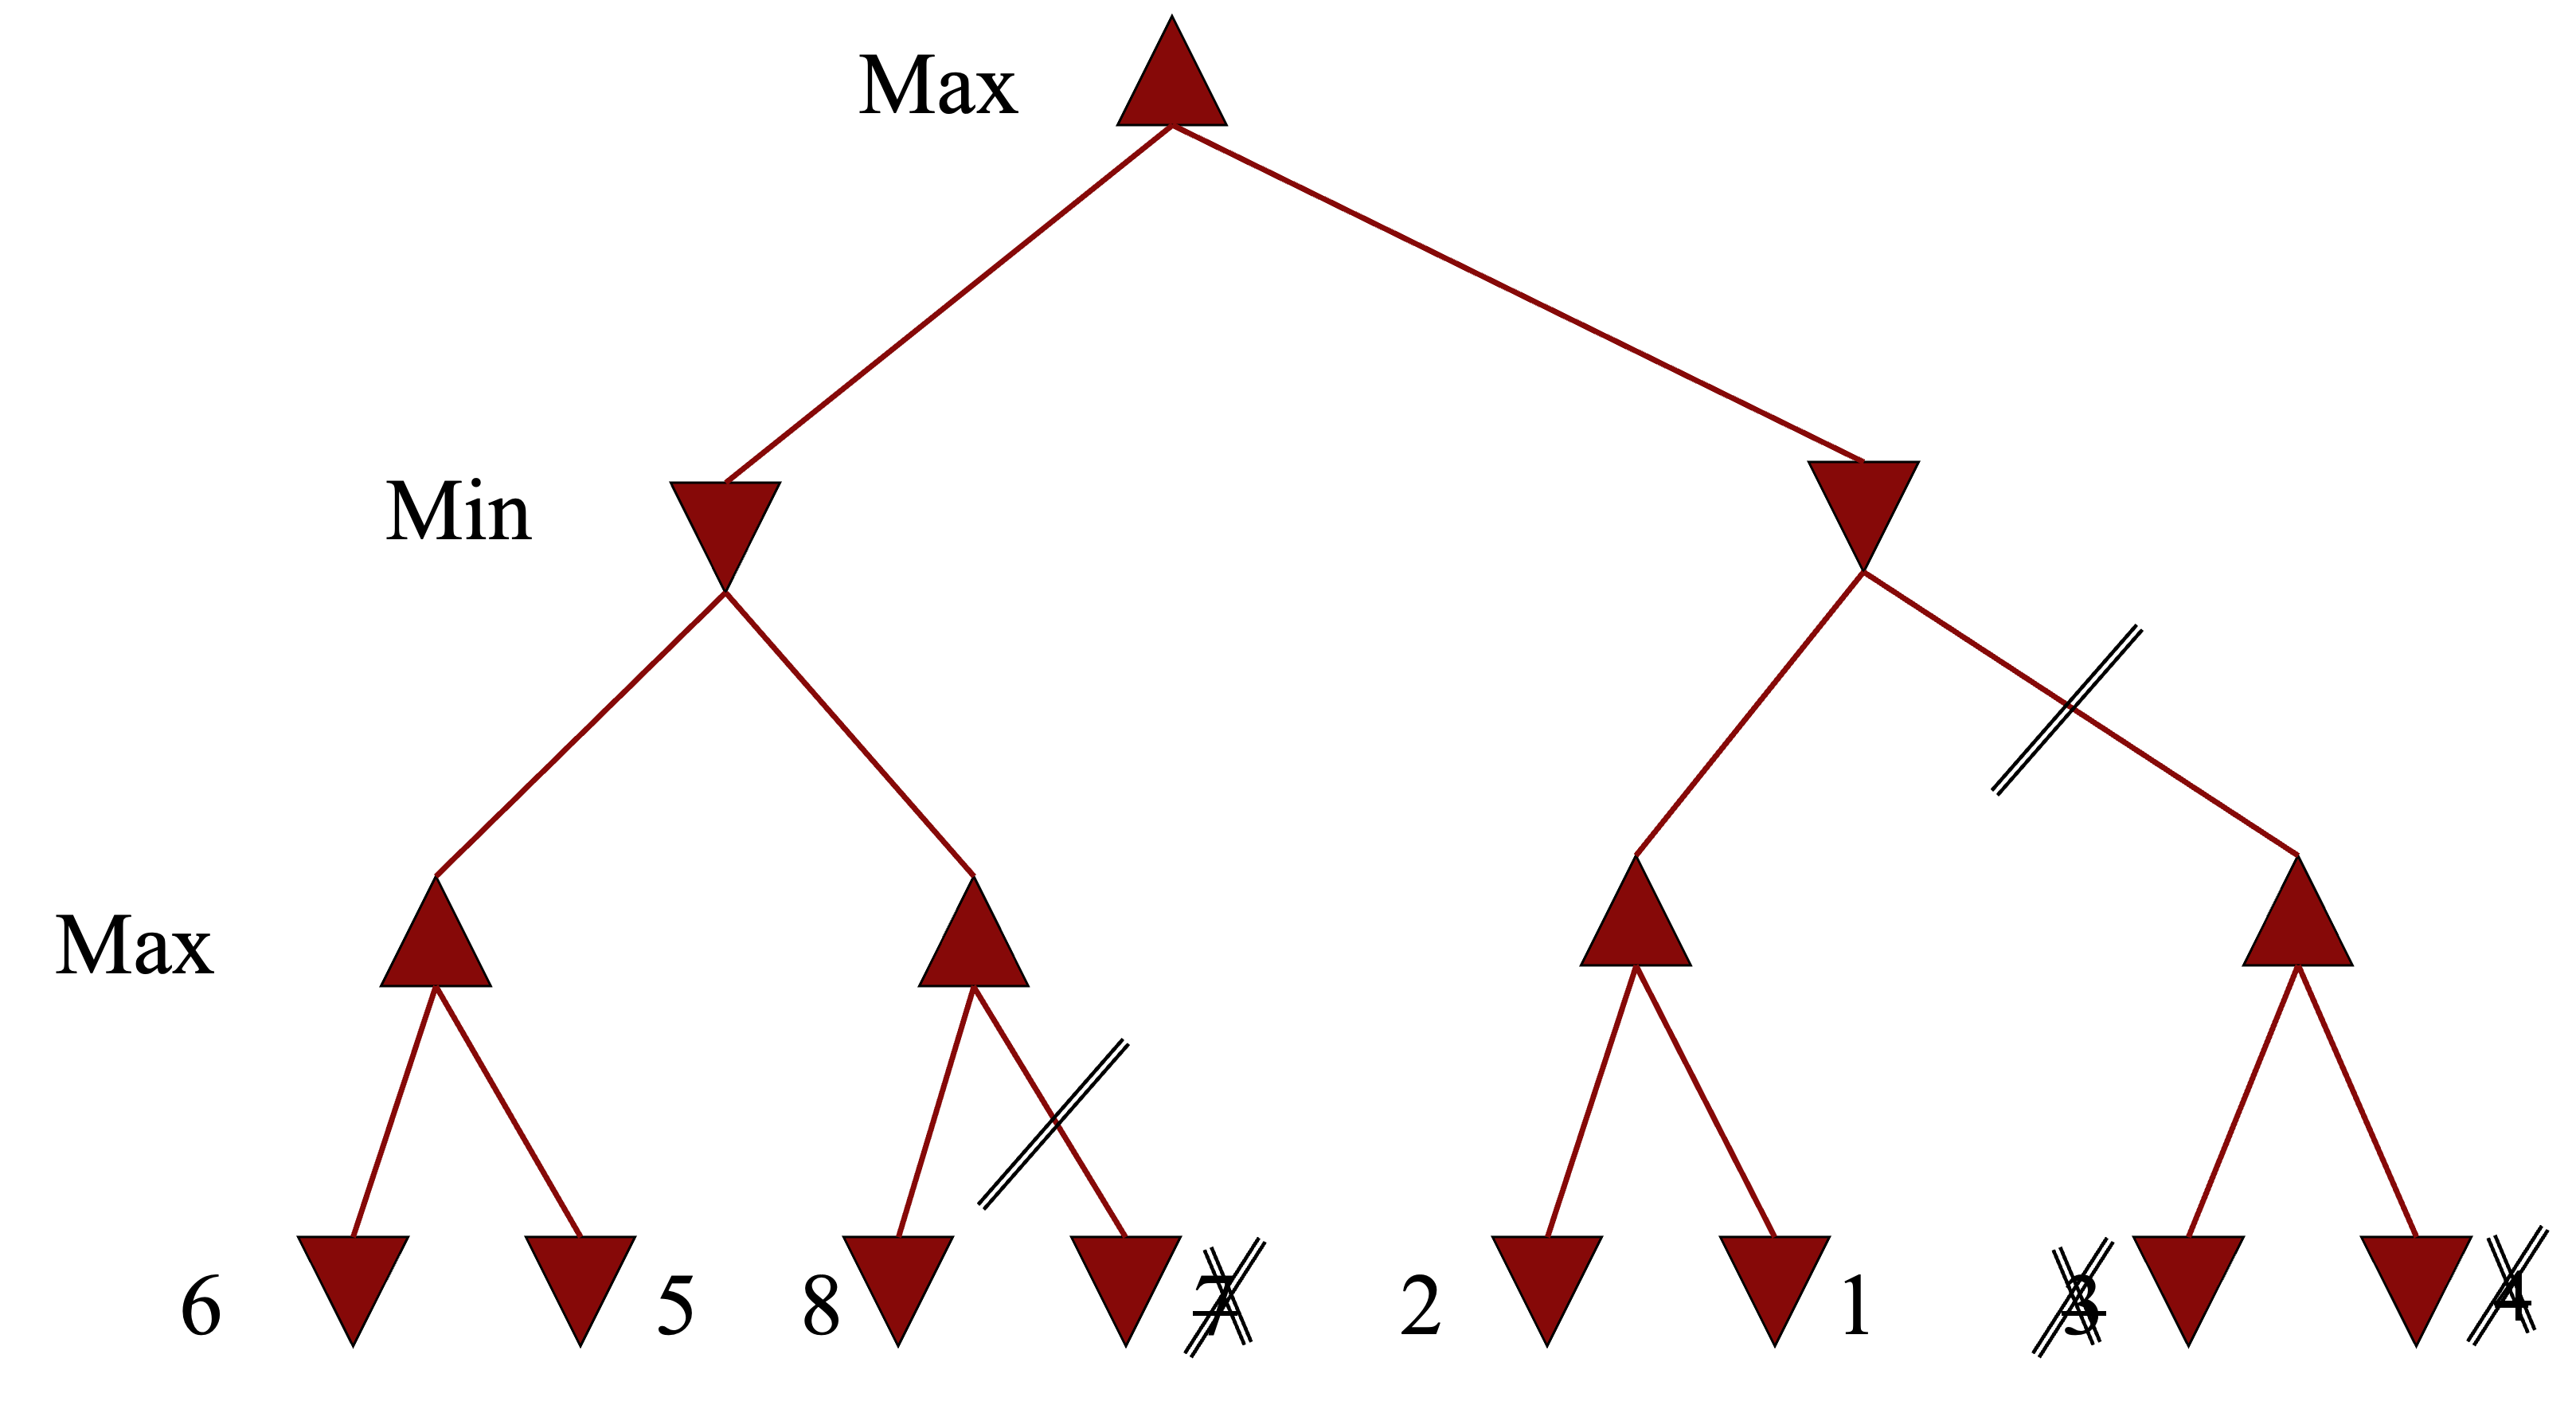
\includegraphics[scale=0.4]{./img/OrdenAlfaBeta3}
\end{figure}
\end{frame} 

%%%%%%%%%%%%%%%%%%%%%%%%%%%%%%%%
%%%%%%%%%%%%%%%%%%%%%%%%%%%%%%%%

\begin{chapter}[images/etsiinformatica4.png]{uicblue}{Búsqueda multiagente \\ 
Funciones de Evaluación}
\end{chapter}

\subsection{Funciones de Evaluación}

%%%%%%%%%%%%%%%%%%%%%%%%%%%%%%%%

\begin{frame} \frametitle{Funciones de Evaluación} \small

\begin{itemize}
    \item Minimax  genera el espacio de búsqueda entero, mientras que el algoritmo alfa-beta podamos partes.
    \item Necesario llegar a estados terminales.
    \item Trabajo shannon (1950) programming a computer for playing chess, propone una función de evaluación heurística a los estados convirtiendo nodos no terminales a terminales.
    \item Sustituye \textbf{función utilidad} por \textbf{función evaluación heurística}, que da una estimación de utilidad de la posición y establecemos un test límite que decide cuando terminar de aplicar función.
    \item Su cálculo ha de ser poco costoso

\end{itemize}
\end{frame} 

%%%%%%%%%%%%%%%%%%%%%%%%%%%%%%%%

\begin{frame} \frametitle{Decisiones imperfectas en juegos de dos adversarios } \small

\begin{itemize}
    \item Decisión imperfecta: Decisión tomada por el algoritmo sobre un horizonte que no alcanza el final del juego (se asume) y con función de evaluación estimada f = û.
    
    \item Función de evaluación, f(n)=  

\begin{enumerate}
    \item si ``n'' no es terminal: (número de filas, columnas o diagonales libres para MAX) -  (número de filas, columnas o diagonales libres para MIN)
    \item si gana MAX: $+ \infty$
    \item si gana MIN: $- \infty$
\end{enumerate}


\begin{figure}
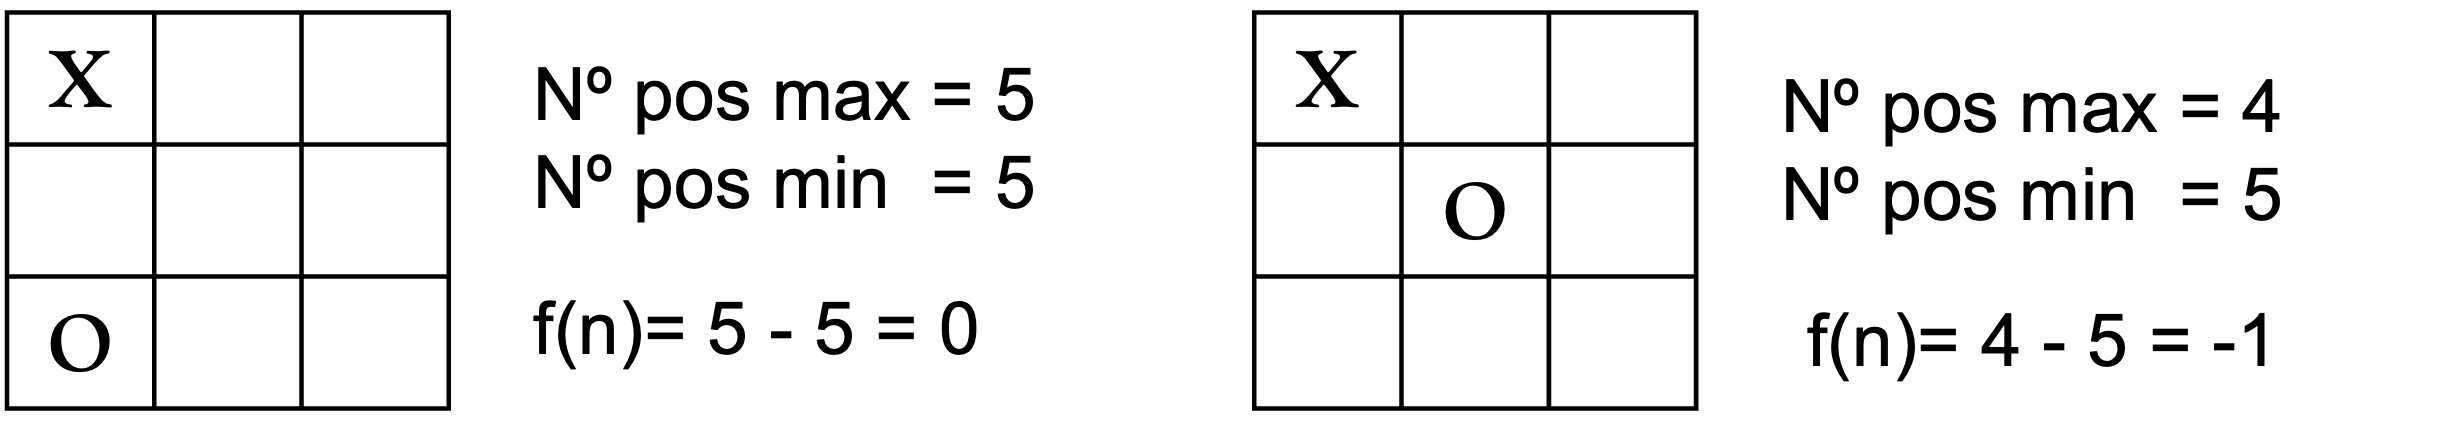
\includegraphics[scale=0.4]{./img/utilidad}
\end{figure}
\end{itemize}
\end{frame} 



%%%%%%%%%%%%%%%%%%%%%%%%%%%%%%%%
%\begin{frame} [fragile ]\frametitle{Puzzle 8 - Heurístico} \footnotesize
%\begin{minted}[fontsize=\small]{python}

%initial_state = '1'
%goal_state = '8'
%problem = ProblemGrafo(initial_state, goal_state)
%solution_node = depth_first_search(problem)
%\end{minted}

%\end{frame} 







%%%%%%%%%%%%%%%%%%%%%%%%%%%%%%%%
%\begin{frame}  \small  
%\end{frame} 


%%%%%%%%%%%%%%%%%%%%%%%%%%%%%%%%
%\begin{frame}  \small  
%\end{frame} 


%%%%%%%%%%%%%%%%%%%%%%%%%%%%%%%%
%\begin{frame}  \small  
%\end{frame} 

%%%%%%%%%%%%%%%%%%%%%%%%%%%%%%%%
%%%%%%%%%%%%%%%%%%%%%%%%%%%%%%%%

%%%%%%%%%%%%%%%%%%%%%%%%%%%%%%%%
%%%%%%%%%%%%%%%%%%%%%%%%%%%%%%%%
   
\backmatter


\end{document}